\documentclass[a4paper,10pt]{article}
\usepackage[pdftex]{graphicx}
\newcommand{\HRule}{\rule{\linewidth}{0.5mm}}
\usepackage{greektex}
\usepackage{hyperref}
\usepackage{listings}
\usepackage{wrapfig}
\usepackage{graphicx}
\usepackage[usenames,dvipsnames]{color}
\usepackage[table]{xcolor}
\usepackage{colortbl}
\usepackage{longtable}
%--------Footers-Headers---------------
\usepackage{fancyhdr}
\pagestyle{fancy}
\fancyhead[LE,RO]{\slshape \rightmark}
\fancyhead[LO,RE]{\slshape \leftmark}
\fancyfoot[C]{\thepage}
%-----Greek language-----------------
\usepackage[cm-default]{fontspec}
\usepackage{xunicode}
\usepackage{xltxtra}
\usepackage{amsmath}
\usepackage{xgreek}
%-----Fonts-------------------------
\setromanfont{FreeSerif}
\setsansfont{FreeSans}
\setmonofont{FreeMono}
%----------Hyper linking setup----------------
\hypersetup{
    bookmarks=false,         % show bookmarks bar?
    unicode=true,          % non-Latin characters in Acrobat’s bookmarks
    pdftoolbar=false,        % show Acrobat’s toolbar?
    pdfmenubar=false,        % show Acrobat’s menu?
    pdffitwindow=false,     % window fit to page when opened
    pdfstartview={FitH},    % fits the width of the page to the window
    pdftitle={My title},    % title
    pdfauthor={Author},     % author
    pdfsubject={Subject},   % subject of the document
    pdfcreator={Creator},   % creator of the document
    pdfproducer={Producer}, % producer of the document
    pdfkeywords={keyword1} {key2} {key3}, % list of keywords
    pdfnewwindow=true,      % links in new window
    colorlinks=true,       % false: boxed links; true: colored links
    linkcolor=black,          % color of internal links
    citecolor=green,        % color of links to bibliography
    filecolor=magenta,      % color of file links
    urlcolor=blue           % color of external links
}
%----------code setup----------------
\lstset{language=verilog,
   keywords={module,initial,forever,begin,wait,case,else,elseif,end,for,function,
      if,assign,while,always,or,posedge,endmodule},
   keywordstyle=\bfseries\color{BrickRed},
   keywords=[2]{wire,input,output,reg},
   keywordstyle={[2]\bfseries\color{OliveGreen}},
   basicstyle=\footnotesize,
   commentstyle=\color{blue},
   stringstyle=\color{black},
   numbers=left,
   numberstyle=\tiny\color{black},
   stepnumber=1,
   numbersep=5pt,
   backgroundcolor=\color{Goldenrod},
   tabsize=5,
   showspaces=false,
   frame=single,
   showtabs=false,
   showstringspaces=false} 


\lstdefinestyle{makefile}
{
    breaklines=true,
    numberblanklines=false,
    language=make,
    tabsize=4,
    keywordstyle=\color{red},
    identifierstyle= %plain identifiers for make
}


%---------image border--------
\usepackage{float}
\floatstyle{boxed} 
\restylefloat{figure}

%---------Figures numbering by section--------
\usepackage{amsmath}
\numberwithin{figure}{section}
\numberwithin{table}{section}


\usepackage{pdfpages}

%opening
%\title{\bf ΛΟΓΙΚΗ ΣΧΕΔΙΑΣΗ 2}
%\author{  Καλάργαρης Χαράλαμποs, AM:3929 \and  Καλάργαρης Χαράλαμποs, AM:3929 \and   Καλάργαρης Χαράλαμποs, AM:3929 }
%\date{27/5/2011}

\begin{document}
\begin{titlepage}

\begin{center}


% Upper part of the page

\includegraphics[width=0.25\textwidth]{/home/federico/Documents/Kile/Diploma/Front_Page/ceid.png}\\[1cm]    
%%/home/federico/Pictures/appmakr-logo.png
\textsc{\LARGE Πανεπιστημίο Πατρών}\\[1.5cm]

\textsc{\Large Μηχανικών Η/Υ και Πληροφορικής}\\[2.5cm]


% Title
\HRule \\[0.4cm]
{ \Large \bfseries Σχεδιασμός System-on-Chip για επεξεργασία εικόνας και υλοποίηση με FPGA. }\\[0.4cm]

\HRule \\[3.5cm]

% Author and supervisor
\begin{minipage}{0.4\textwidth}
\begin{flushleft} \large
\emph{Author:}\\
Χαράλαμπος \textsc{Καλάργαρης}
\end{flushleft}
\end{minipage}
\begin{minipage}{0.4\textwidth}
\begin{flushright} \large
\emph{Supervisor:} \\
Θεμιστοκλής \textsc{Χανιωτάκης}
\end{flushright}
\end{minipage}

\vfill

% Bottom of the page
{\large \today}

\end{center}

\end{titlepage}
%\maketitle
\newpage
\newpage\mbox{}\newpage

Για την  εκπόνηση αυτής της διπλωματικής θα ήθελα να ευχαριστήσω ιδιαίτερα τον καθηγητή μου κ.Χανιωτάκη που ήταν υπεύθυνος της εργασίας και τον κ.Αδαό για την πολύτιμη βοήθειά του στο εργαστήριο Μικροηλεκτρονικής. Παράλληλα θα ήθελα να ευχαριστήσω τον κ.Αλεξιού που είναι υπεύθυνος του εργαστηρίου Μικροηλεκτρονικής. Τέλος θα ήθελα να ευχαριστήσω την οικογένειά μου για την στήριξή τους όλα αυτά τα χρόνια που σπούδασα στην Πάτρα.



\newpage\mbox{}\newpage
\tableofcontents
\newpage
\listoffigures
\newpage
\listoftables
\newpage
\newpage
\section{Εισαγωγή}



\paragraph{\newline\newline Σκοπός\newline\newline}

Ο σκοπός αυτής της διπλωματικής εργασίας είναι να δημιουργηθεί ένα System On Chip (SoC) που θα στοχεύει στην επεξεργασία εικόνας. Ουσιαστικά στόχος μας είναι να αναβαθμίσουμε την ήδη υπάρχουσα πλατφόρμα που υπάρχει στο εργαστήριο Μικροηλεκτρονικής. Αυτό θα γίνει με την αλλαγή του επεξεργαστή LEON2 που χρησιμοποιείται τώρα με τον επεξεργαστή OR1200 που παρέχεται ελεύθερα από το Open Cores. Οι κυριότεροι λόγοι που για τους οποίους κρίθηκε αναγκαία αυτή η αλλαγή φαίνονται παρακάτω.
\begin{itemize}
 \item O LEON2 είναι ένας επεξεργαστής που το πρώτο μοντέλο του σχεδιάστηκε το 1997. Τα τελευταία χρόνια όμως οι αναβαθμίσεις που εμφανίζονται για αυτόν τον επεξεργαστή αλλά και η χρησιμοποίησή του σε μοντέρνα ολοκληρωμένα συστήματα ακολουθούν μια φθίνουσα πορεία.
 \item Σε αντίθεση με το παραπάνω στοιχείο ο επεξεργαστής OR1200 ακολουθεί μία ανοδική πορεία τα τελευταία χρόνια. Οι κυριότεροι λόγοι αυτής της ανόδου έχουν να κάνουν με το γεγονός ότι o OR1200 είναι ένας επεξεργαστής ελεύθερου λογισμικού με αποτέλεσμα οι περισσότερες ακαδημαϊκές κοινότητες στον κόσμο να τον χρησιμοποιούν για να αναπτύξουν εφαρμογές και να βοηθήσουν τους νέους φοιτητές να εξοικειωθούν με την αρχιτεκτονική RISC στους επεξεργαστές.
 \item Το μεγαλύτερο πλεονέκτημα του επεξεργαστή OR1200 έχει να κάνει με το γεγονός ότι μπορεί κάποιος να σχεδιάσει το δικό του σύστημα χωρίς να χρησιμοποιήσει εμπορικά προϊόντα που κοστίζουν αφού τόσο ο επεξεργαστής όσο και ο δίαυλος επικοινωνίας (Wishbone) είναι ελεύθερα προϊόντα που διανέμονται από το OpenCores.
 \item Τέλος ο επεξεργαστής ΟR1200 λόγο του τρόπου που έχει σχεδιαστεί προσφέρει στον χρήστη μια πληθώρα από επιλογές για την παραμετροποίηση του. Αυτό έχει δυο θετικά στοιχεία. Το πρώτο έχει να κάνει με το γεγονός ότι λόγω της εύκολης αλλά ταυτόχρονα και μεγάλης παραμετροποίησης που παρέχει στον χρήστη, τον κάνει να απευθύνεται σε ένα μεγάλο φάσμα εφαρμογών ειδικού σκοπού. Το δεύτερο πλεονέκτημα απευθύνεται στην χρησιμότητα της παραμετροποίηση για τους νέους φοιτητές. Οι φοιτητές μπορούν μέσω της παραμετροποίησης του επεξεργαστή να ακολουθήσουν πολλά διαφορετικά σενάρια υλοποίησης γεγονός που τους βοηθά σημαντικά στην καλύτερη κατανόηση της αρχιτεκτονικής RISC επεξεργαστών. 
\end{itemize}

\newpage
\paragraph{\newline\newline Περιορισμοί - Τελικός Σκοπός\newline\newline}

Όπως γίνετε εύκολα κατανοητό η δημιουργία ενός ολοκληρωμένου συστήματος είναι μία πολύ χρονοβόρα διαδικασία που απαιτεί την συνεργασία πολλών ανθρώπων για να επιτευχθεί. Επειδή η διπλωματικές εργασίες είναι ατομικές έπρεπε αρχικά να οριστεί ποίος θα ήταν ο στόχος αυτής της διπλωματικής εργασίας. Έτσι μετά από συνεννόηση με τον κ.Χανιωτάκη και τον κ.Αδαό ορίστηκε σαν στόχος η δημιουργία ενός απλοϊκού συστήματος που θα ενσωματώνει τον καινούργιο επεξεργαστή ΟR1200, τον δίαυλο επικοινωνίας AMBA AHB και μία απλή μνήμη. Με αυτό τον τρόπο δημιουργούμε την βάση του μεγαλύτερου συστήματος που είναι απώτερος σκοπός του εργαστήριο Μικροηλεκτρονικής. Ουσιαστικά μετά την εκπόνηση και άλλων διπλωματικών εργασιών (που θα δημιουργούν άλλες μονάδες για το σύστημα- όπως για επεξεργασία εικόνας) θα είναι δυνατόν να προσθέσουν τις μονάδες που σχεδίασαν πάνω στο σύστημα που εμείς σχεδιάσαμε με αποτέλεσμα να δημιουργηθεί ένα μεγαλύτερο και πολυπλοκότερο σύστημα.
\newline

 Για να εξασφαλίσουμε την δυνατότητα σε άλλους φοιτητές να σχεδιάζουν τις μονάδες που θέλουν και να τις βάζουν κατευθείαν πάνω στο σύστημα μας, στόχος μας είναι να αλληλεπιδρά αρμονικά το σύστημα με την μνήμη που έχει. Αυτό διασφαλίζει την παραπάνω δυνατότητα για τον λόγο ότι τόσο η μνήμη όσο και οι μονάδες που θα σχεδιάσουν οι φοιτητές θα έχουν τα ίδια σήματα εξόδου και εισόδου πάνω στο δίαυλο επικοινωνίας. Με αυτόν τρόπο εμείς διασφαλίζουμε στους φοιτητές ότι αν σχεδιάσουν σωστά την μονάδα τους και ακολουθήσουν την λογική που απαιτεί ο δίαυλος AMBA AHB τότε η μονάδα τους θα αλληλεπιδρά ορθά με το επεξεργαστή ΟR1200.


\paragraph{\newline\newline Συνδρομή στο έργο της Ακαδημαϊκής κοινότητας \newline\newline}

Ένα από τα σημαντικότερα αποτελέσματα αυτής της διπλωματικής εργασίας είναι η συνδρομή της στο έργο της ακαδημαϊκής κοινότητας. Μέτα το τέλος της διπλωματικής εργασίας τόσο οι φοιτητές όσο και οι καθηγητές του τμήματος Μηχανικών Ηλεκτρονικών Υπολογιστών και Πληροφορικής και κυρίως αυτοί που θα ασχοληθούν με το εργαστήριο Μικροηλεκτρονικής θα έχουν στην διάθεσή τους ένα καινούργιο επεξεργαστή για να μπορούν να πειραματιστούν. Αυτή η αλλαγή θα βοηθήσει τόσο το τμήμα όσο και το εργαστήριο Μικροηλεκτρονικής να αναβαθμίσουν τα εργαλεία που παρέχουν στους φοιτητές και ταυτόχρονα να διευρύνουν το πεδίο γνώσης που προσφέρουν.
\newline

Παράλληλα το έργο αυτής της διπλωματικής εργασίας θα συμπεριληφθεί σε μία δημοσίευση που θα γίνει στο παγκόσμιο συμπόσιο της ΙΕΕΕ 2012 με θέμα Rapid System Prototyping. To συμπόσιο θα γίνει στην πόλη Tempere της Φιλανδίας και το θέμα τις δικής μας δημοσίευσης είναι "A Flexible Platform for Developing and Evaluating System-on-Chip Architectures". Οι υπόλοιποι συγγραφείς αυτής της δημοσίευσης φαίνονται παρακάτω.
\newpage
\begin{itemize}
 \item Κωνσταντίνος Αδαός.
 \item Βαγγέλης Μαριάτος.
 \item Γεώργιος Π.Αλεξιού.
\end{itemize}


\paragraph{\newline\newline Μορφή Αναφοράς Διπλωματικής εργασίας\newline\newline}

Η αναφορά αυτής της διπλωματικής εργασίας δημιουργήθηκε με τέτοιο τρόπο ώστε παρουσιάσει τόσο το έργο που έγινε για την εκπόνηση της όσο και για να αποτελεί ενα εγχειρίδιο χρήσης για τους φοιτητες της σχολής που θέλουν να ασχοληθούν με τον επεξεργαστή OR1200. Ουσιαστικά η διπλωματική εργασία χωρίζεται σε 3 κομμάτια. 

\begin{enumerate}
 \item Το πρώτο εστιάζει στην περιγραφή των κυριότερων χαρακτηριστικών του επεξεργαστή ΟR1200 που συλλέχθηκαν μέσα από πολλά διαφορετικά εγχειρίδια και αποτελούν μια πολύ καλή εισαγωγή για τους φοιτητές πάνω σε θέματα αρχιτεκτονικής του OR1200. 
 \item To δεύτερο αναφέρεται τόσο στον τρόπο που εγκαταστάθηκαν οι κατάλληλες αλυσίδες προγραμμάτων στο εργαστήριο Μικροηλεκτρονικής όσο και ο τρόπος με τον οποίο χρησιμοποιούνται αυτά τα προγράμματα για να προσομοιώσουμε την λειτουργιά του επεξεργαστή. Διαδικασία που είναι απαραίτητη για τους νέους φοιτητές ώστε να είναι πιο εύκολη η εισαγωγή και η κατανόηση του επεξεργαστή OR1200.  
 \item To τελευταίο κομμάτι εστιάζει στην δημιουργία του ολοκληρωμένου συστήματος. Ουσιαστικά αποτελεί μια παρουσίαση των παραπάνω κομματιών σε πραγματικό κύκλωμα με παράδειγμα. Ταυτόχρονα περιγράφει τις δυσκολίες που συναντήθηκαν κατά την δημιουργία του ολοκληρωμένου συστήματος.
\end{enumerate}



\newpage
\newpage
\section{OpenRISC 1200 IP Core}
Αυτό το κεφάλαιο αποτελεί μια πρώτη γνωριμία με τον επεξεργαστή OR1200. Θα παρουσιαστούν τα κυριότερα χαρακτηριστικά του και ο τρόπος με τον οποίο υλοποιούνται τόσο από την μεριά του υλικού όσο και από την μεριά της λογικής την οποία ακολουθούν. Κυριότερος σκοπός του κεφαλαίου αυτού είναι να παρέχει στον χρήστη την απαραίτητη γνώση που θα τον βοηθήσει στην ανάπτυξη εφαρμογών σε συμβολική γλώσσα αλλά και στο πως μπορεί να αποτελέσει μέρος ενός ολοκληρωμένου κυκλώματος ειδικού σκοπού (ASIC).

\subsection{Εισαγωγή}

Σε αυτή την ενότητα θα παρουσιαστούν τα κυριότερα χαρακτηριστικά της οικογένειας επεξεργαστών OpenRISC 1000 και του επεξεργαστή OR1200 που αποτελεί μέρος της.

\subsubsection{OpenRISC Οικογένεια}
Η OpenRISC 1000 οικογένεια επεξεργαστών αναφέρεται σε μια ελεύθερη, ανοιχτού
λογισμικού RISC αρχιτεκτονική κεντρικών μονάδων επεξεργασίας. Σχετικά με την
αρχιτεκτονική, η OpenRISC 1000 οικογένεια στοχεύει σε ένα φάσμα υλοποιήσεων που	
ποικίλουν ως προς την τιμή/απόδοση και το είδος της εφαρμογής. Είναι μια 
32/64-bit φόρτωσης και αποθήκευσης (load and store) RISC αρχιτεκτονική που σχεδιάστηκε
με έμφαση στην απόδοση, στην απλότητα, στην χαμηλή ενεργειακή κατανάλωση, στην επεκτασιμότητα
και στην ευελιξία. Η OpenRISC αρχιτεκτονική στοχεύει σε μεσαία και υψηλή απόδοση
δικτύωσης (networking), σε ενσωματωμένα, αυτοκινητοβιομηχανικά και φορητά υπολογιστικά περιβάλλοντα. 

\vspace{0.7cm}
\begin{figure}[h!]
 \centering
 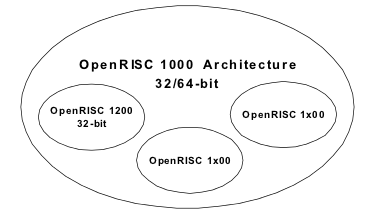
\includegraphics[bb=0 0 376 214,scale=0.7]{/home/federico/Documents/Kile/Diploma/Images/OR_family.png}
 % OR_family.png: 376x214 pixel, 72dpi, 13.26x7.55 cm, bb=0 0 376 214
 \caption{Σχηματική αναπαράσταση OpenRISC αρχιτεκτονικής.}
\end{figure}
\vspace{0.7cm}


Όλες οι OpenRISC υλοποιήσεις που το πρώτο ψηφίο στον αριθμό ταυτότητας
(identification number) είναι '1' ανήκουν στην 
OpenRISC 1000 οικογένεια. Το δεύτερο ψηφίο ορίζει ποια χαρακτηριστικά της OpenRISC
1000 αρχιτεκτονικής είναι υλοποιημένα και με ποιο τρόπο είναι υλοποιημένα. Τα δύο
τελευταία ψηφία αναφέρονται στο πως μια υλοποίηση ήταν παραμετροποιημένη πριν 
χρησιμοποιηθεί σε πραγματική εφαρμογή. 

\subsubsection{OpenRISC 1200}
 Ο OR1200 είναι ενας 32-bit βαθμωτός RISC επεξεργαστής με Harvard μικρο-αρχιτεκτονική, 5 stage integer pipeline, υποστήριξη εικονικής μνήμης (MMU) και βασικές δυνατότητες
DSP. 
\newline

Οι προκαθορισμένες κρυφές μνήμες είναι:
\begin{itemize}
 \item 1-way direct-mapped 8KB κρυφή μνήμη δεδομένων. 
 \item 1-way direct-mapped 8KB κρυφή μνήμη εντολών. 
 \item Κάθε κρυφή μνήμη έχει γραμμή μεγέθους 16-byte. 
 \item Και οι δύο κρυφές μνήμες είναι φυσικά υλοποιημένες. 
\end{itemize}

Η προκαθορισμένη MMU αποτελείται από:
\begin{itemize}
 \item 64-entry hash based 1-way direct-mapped data TLB. 
 \item 64-entry hash based 1-way direct-mapped instruction TLB. 
\end{itemize}

Μερικές άλλες επιπρόσθετες λειτουργίες που παρέχει ο OpenRISC 1200 είναι η μονάδα
αποσφαλμάτωσης πραγματικού χρόνου (real-time debug unit), υψηλής ανάλυσης χρονιστή, προγραμματιζόμενο ελεγκτή διακοπών (programmable interrupt controller) και μονάδα
ρύθμισης των ενεργειακών απαιτήσεων. 
\newline

Ο OR1200 ουσιαστικά προορίζεται για εφαρμογές σε ενσωματωμένα, φορητά και δικτύωσης
συστήματα. Μπορεί να ανταγωνιστεί τους τελευταίους βαθμωτούς 32-bit RISC επεξεργαστές
της κλάσης του και να υποστηρίξει αποδοτικά οποιοδήποτε μοντέρνο λειτουργικό σύστημα. 
Ανταγωνιστές του θεωρούνται οι ARM10, ARC και Tensilica RISC επεξεργαστές. 
\newline
Συνοπτικά παρουσιάζονται παρακάτω τα χαρακτηριστικά του OR1200:
{%
\renewcommand{\arraystretch}{1.2}
\newcommand{\mc}[3]{\multicolumn{#1}{#2}{#3}}
\definecolor{tcD}{rgb}{0.968627,0.968627,0.968627}
\definecolor{tcA}{rgb}{1,1,0}
\definecolor{tcB}{rgb}{0.968627,0.968627,0.968627}
\definecolor{tcC}{rgb}{1,1,0.772549}
\begin{table}
\begin{center}
\begin{tabular}{ll}
% use packages: color,colortbl
\rowcolor{tcA}
  & \textbf{OR 1200}\\
\rowcolor{tcD}
\textbf{License} & \textit{GNU LGPL}\\
\rowcolor{tcC}
\textbf{Platform} & \textit{FPGA, ASIC}\\
\mc{1}{>{\columncolor{tcB}}l}{\textbf{Distributed file format}} & \mc{1}{>{\columncolor{tcD}}l}{\textit{Verilog}}\\
\rowcolor{tcC}
\textbf{General} &  \\
\rowcolor{tcD}
Architecture & \textit{32-bit RISC}\\
\rowcolor{tcC}
Byte Ordering & \textit{Big endian}\\
\rowcolor{tcD}
Pipeline depth & \textit{5}\\
\rowcolor{tcC}
Issue type & \textit{Single}\\
\rowcolor{tcD}
\textbf{Register file} &  \\
\rowcolor{tcC}
Organization & \textit{Flat}\\
\rowcolor{tcD}
\# of global registers & \textit{32}\\
\rowcolor{tcC}
Total \# of GPRs & \textit{32}\\
\rowcolor{tcD}
\textbf{ISA} &  \\
\rowcolor{tcC}
Type & \textit{ORBIS32}\\
\rowcolor{tcD}
Addressing modes & \textit{Immediate,
displacement, pcrelative}\\
\rowcolor{tcC}
MAC & \textit{32x32-bit, 48-bit Acc}\\
\rowcolor{tcD}
Custom instructions & \textit{Yes}\\
\rowcolor{tcC}
Custom coprocessor & \textit{Yes}\\
\rowcolor{tcD}
Software floating-point support & \textit{IEEE-754 Single and double precision}\\
\rowcolor{tcC}
\textbf{Cache} &  \\
\rowcolor{tcD}
Hierarchy & \textit{Harvard}\\
\rowcolor{tcC}
Instruction cache
size & \textit{512 byte-8 Kbyte}\\
\rowcolor{tcD}
Data cache size & \textit{4-8 Kbyte}\\
\rowcolor{tcC}
Line size & \textit{8-16 byte}\\
\rowcolor{tcD}
Placement scheme & \textit{Direct-mapped}\\
\rowcolor{tcC}
Valid bits & \textit{One per cache line}\\
\rowcolor{tcD}
Line-locking & \textit{Set basis}\\
\rowcolor{tcC}
\textbf{System Interface} & \textit{Wishbone SoC rev. B 32-bit}\\
\rowcolor{tcD}
\textbf{Power Management} & \textit{Slow and idle mode, sleep mode, doze mode}\\
\rowcolor{tcC}
\textbf{Memory} &  \\
\rowcolor{tcD}
On-chip RAM & \textit{Configurable} \\
\rowcolor{tcC}
\textbf{Operating system
support} & \textit{Linux, uClinux, OAR RTEMS RTOS}\\
\end{tabular}
\end{center}
\caption{Overview of OR1200 specifications}
\end{table}
}%
\newpage


\subsection{Αρχιτεκτονική}
Στο παρακάτω σχήμα βρίσκεται η σχηματική αναπαράσταση του OR1200 επεξεργαστή (δεν απεικονίζεται η μονάδα FPU) 
όπου αποτελείται από τις εξής υπομονάδες:
\begin{itemize}
 \item CPU/FPU/DSP central block.
 \item Direct-mapped data cache.
 \item Direct-mapped instruction cache.
 \item Data MMU based on hash based DTLB.
 \item Instruction MMU based on hash based ITLB.
 \item Power management unit and power management interface.
 \item Tick timer.
 \item System Interface.
 \item Debug unit and development interface.
 \item Interrupt controller and interrupt interface.
 \item Instruction and Data WISHBONE host interfaces.
\end{itemize}
\begin{figure}[h!]
 \centering
 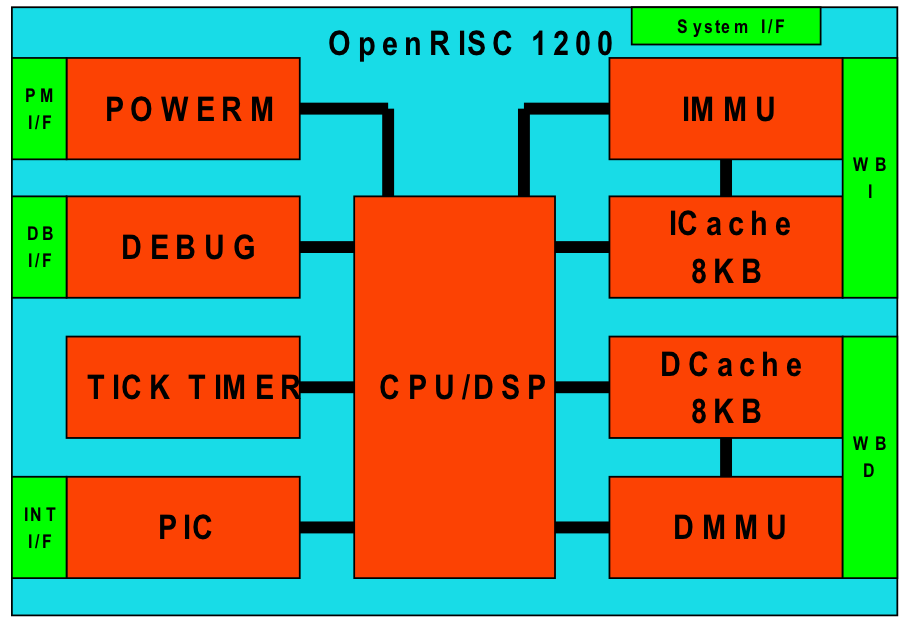
\includegraphics[bb=0 0 905 625,scale=0.3]{/home/federico/Documents/Kile/Diploma/Images/or1200.png}
 % or1200.png: 905x625 pixel, 72dpi, 31.93x22.05 cm, bb=0 0 905 625
 \caption{Core's Architecture}
\end{figure}

\subsubsection{CPU/FPU/DSP}
Το μπλόκ CPU/FPU/DSP είναι ένα κεντρικό κομμάτι του επεξεργαστή OR1200 RISC. Το σχήμα 2.3 δείχνει
το βασικό μπλόκ διάγραμμα του CPU/FPU/DSP. Η μονάδα του OR1200 CPU/FPU/DSP
υλοποιεί μόνο τις ORBIS32 και ORFPX32 ομάδες εντολών. Δεν υπάρχει ακόμα υλοποίηση για τις
ομάδες εντολών ORBIS64, ORFBX64 και ORVDX64.

\vspace{0.7cm}
\begin{figure}[h!]
 \centering
 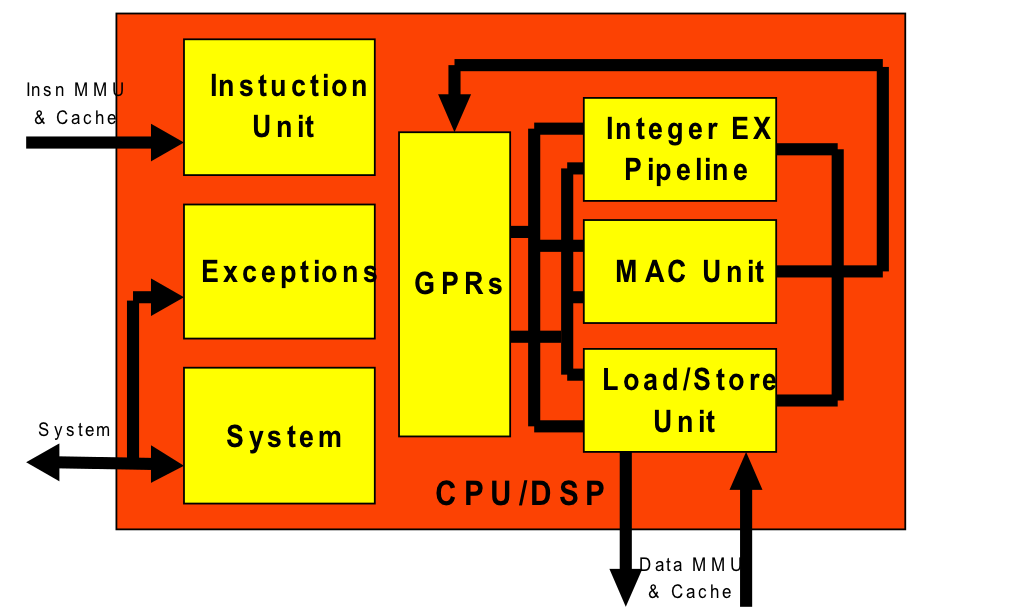
\includegraphics[bb=0 0 1020 613,scale=0.35]{./Images/cpu-dsp.png}
 % cpu-dsp.png: 1020x613 pixel, 72dpi, 35.98x21.63 cm, bb=0 0 1020 613
 \caption{CPU/DSP block diagram.}
\end{figure}

\vspace{0.7cm}

\paragraph{Μονάδα Εντολών\newline\newline}

Η μονάδα εντολών (instruction unit) υλοποιεί την βασική pipeline διαδικασία, φέρνει τις
εντολές από το υποσύστημα της μνήμης, τις αποστέλλει στις διαθέσιμες μονάδες εκτέλεσης (execution unit)
και διατηρεί ενα ιστορικό καταστάσεων ώστε να εξασφαλίσει ένα ακριβές μοντέλο εξαιρέσεων (exception model)
για τον σωστό τερματισμό των εργασιών. Επίσης εκτελεί τις υπό όρους και άνευ όρων εντολές διακλάδωσης.
\newline

Παράλληλα μπορεί να στείλει διαδοχικές εντολές σε κάθε ρολόι αν η κατάλληλη μονάδα εκτέλεσης
είναι διαθέσιμη. Η μονάδα εκτέλεσης είναι αυτή που πρέπει να διακρίνει αν τα δεδομένα που χρειάζεται
η εντολή είναι διαθέσιμα και να διασφαλίσει ότι καμία άλλη εντολή δεν χρησιμοποιεί εκείνη την
στιγμή τον ίδιο καταχωρητή. Επιπρόσθετα υπολογίζει την αποτελεσματική διεύθυνση (effective address)
και προσκομίζει την εντολή από την κρυφή μνήμη εντολών σε ένα κύκλο ρολογιού.  Ύστερα η
αποτελεσματική διεύθυνση μετατρέπεται σε φυσική διεύθυνση με την βοήθεια της IMMU μονάδας. 
\newline

Τέλος η μονάδα εντολών χειρίζεται μόνο τις εντολές της κλάσης ORBIS32 και κατά επιλογή ένα
υποσύνολο των εντολών ORFPX32. Μερικές εντολές της κλάσης ORFPX32  και όλες οι εντολές
των ORFPX3264 και ORVDX64 δεν υποστηρίζονται ακόμα από τον OR1200. Παρακάτω παρουσιάζεται 
συνοπτικά η λίστα των εντολών που υποστηρίζει o OR1200 και ποιες είναι προαιρετικές (optional).  
Για την πλήρη περιγραφή κάθε εντολής μπορείτε να ανατρέξετε στο εγχειρίδιο 
OpenRISC 1000 System Architecture Manual.

\vspace{0.7cm}
\renewcommand{\arraystretch}{1.2}
\setlength{\tabcolsep}{0.2em}
\definecolor{tcA}{rgb}{1,1,0}
\begin{table}[h!]
\begin{center}
\begin{tabular}{|c|c|c|c|c|c|c|c|}
% use packages: color,colortbl
\hline
\rowcolor{tcA}
\bf{Instruction} & \bf{Opt.} & \bf{Instruction} & \bf{Opt.} & \bf{Instruction} & \bf{Opt.} & \bf{Instruction} & \bf{Opt.}\\
\rowcolor{tcA}
\bf{mnemonic} &   & \bf{mnemonic}&   & \bf{mnemonic} &   & \bf{mnemonic} &  \\\hline
l.add &  & l.macrc & Y & l.sh &  & lf.sflt.s & Y\\\hline
l.addc & Y & l.msb & Y & l.sll &  & lf.sfne.s & Y\\\hline
l.addi &  & l.mfspr &  & l.slli &  & lf.sub.s & Y\\\hline
l.and &  & l.movhi &  & l.sra &  &  & \\\hline
l.andi &  & l.mtspr &  & l.srai &  &  & \\\hline
l.bf &  & l.mul & Y & l.srl &  &  & \\\hline
l.bnf &  & l.muli & Y & l.srli &  &  & \\\hline
l.div & Y & l.nop &  & l.sub & Y &  & \\\hline
l.ff1 & Y & l.or &  & l.sw&  &  & \\\hline
l.fl1 & Y & l.ori &  & l.sys &  &  & \\\hline
l.j &  & l.rfe &  & l.trap &  &  & \\\hline
l.jal &  & l.rori &  & l.xor &  &  & \\\hline
l.jalr &  & l.sb &  & l.xori &  &  & \\\hline
l.jr &  & l.sfeq &  & lf.add.s & Y &  & \\\hline
l.lbs &  & l.sfges &  & lf.div.s & Y &  & \\\hline
l.lbz &  & l.sfgeu &  & lf.ftoi.s & Y &  & \\\hline
l.lhs &  & l.sfgts &  & lf.itof.s & Y &  & \\\hline
l.lhz &  & l.sfgtu &  & lf.mul.s & Y &  & \\\hline
l.lws &  & l.sfleu &  & lf.sfeq.s & Y &  & \\\hline
l.lwz &  & l.sflts &  & lf.sfge.s & Y &  & \\\hline
l.mac & Y & l.sfltu &  & lf.sfgt.s & Y &  & \\\hline
l.maci & Y & l.sfne &  & lf.sfle.s & Y &  & \\\hline
\end{tabular}
\end{center}
\caption{Λίστα εντολών OR1200.}
\end{table}
\newpage

\paragraph{Καταχωρητές Γενικού Σκοπού\newline\newline}

Ο OpenRISC 1200 χρησιμοποιεί 32 καταχωρητές γενικού σκοπού (general-purpose registers) των 32 δυαδικών ψηφίων. Η αρχιτεκτονική του επίσης υποστηρίζει σκιώδη αντίγραφα (shadow copies) του αρχείου καταχωρητών (register file)
ώστε να υλοποιεί γρήγορη εναλλαγή μεταξύ των πλαισίων εργασίας (working contexts), όμως
αυτή η λειτουργία δεν υποστηρίζεται από την παρούσα υλοποίηση του OR1200.
\newline

Ο OR1200 υλοποιεί το αρχείο καταχωρητών γενικού σκοπού σαν δυο σύγχρονες μνήμες διπλής θύρας
με χωρητικότητα 32 λέξεων των 32 bit  ανά λέξη. Παράλληλα έχει την δυνατότητα να διαβάζει
δύο τελούμενα σε κάθε κύκλο ρολογιού και να αποθηκεύει ένα αποτέλεσμα καταχωρητές προορισμού.
\newpage
\paragraph{Μονάδα Load/Store\newline\newline}

Η μονάδα Load/Store (LSU) μεταφέρει όλα τα δεδομένα μεταξύ των καταχωρητών γενικού σκοπού (GPRs) και τον
επεξεργαστή διαμέσου του εσωτερικού διαύλου επικοινωνίας. Έχει υλοποιηθεί σαν μια ανεξάρτητη μονάδα
εκτέλεσης ώστε οι καθυστερήσεις στο υποσύστημα μνήμης λόγω εξαρτήσεων μεταξύ δεδομένων να
επηρεάζει μόνο την pipeline διαδικασία.
\newline

Τα κυριότερα χαρακτηριστικά της μονάδας Load/Store παρουσιάζονται παρακάτω:


\begin{itemize}
 \item όλες οι εντολές Load/Store είναι υλοποιημένες σε επίπεδο hardware (atomic instructions include)
 \item pipeline λειτουργία
 \item ευθυγραμμισμένες προσπελάσεις στην μνήμη
 \item address entry buffer
\end{itemize}

Όταν κάποια εντολή Load ή Store προορίζεται για εκτέλεση τότε η μονάδα Load/Store (LSU)
διερευνά αν όλα τα τελούμενα είναι διαθέσιμα. Τα τελούμενα που ελέγχει είναι τα παρακάτω:


\begin{itemize}
 \item Οι διευθύνσεις των καταχωρητών που θα χρησιμοποιηθούν.
 \item Τα δεδομένα στους καταχωρητές που προορίζονται για εκτέλεση (store εντολή).
 \item Τα δεδομένα στους καταχωρητές που προορίζονται για αποθήκευση (load εντολή).
\end{itemize}


Η μονάδα Load/Store εκτελεί μια εντολή load κάθε δύο κύκλους ρολογιού, υποθέτοντας ότι 
έχουμε ευστοχία στην κρυφή μνήμη δεδομένων. Η εκτέλεση της εντολής store απαιτεί ένα 
κύκλο ρολογιού, υποθέτοντας πάλι ότι έχουμε ευστοχία στην κρυφή μνήμη δεδομένων. Παράλληλα
η μονάδα Load/Store υπολογίζει τις αποτελεσματικές διευθύνσεις (effective address), οι
οποίες αργότερα μετατρέπονται σε φυσικές διευθύνσεις με την της DMMU μονάδας.

\paragraph{Πράξεις ακεραίων\newline\newline}

Ο πυρήνας του OR1200 υποστηρίζει τα παρακάτω είδη εντολών για πράξεις μεταξύ 32 bit ακεραίων (integer execution pipeline):
\begin{itemize}
 \item Αριθμητικές εντολές.
 \item Εντολές σύγκρισης.
 \item Λογικές εντολές.
 \item Εντολές ολίσθησης και περιστροφής.
\end{itemize}

\vspace{0.7cm}
\definecolor{tcA}{rgb}{1,1,0}
\begin{table}[h!]
\begin{center}
\begin{tabular}{|l|c|}\hline
% use packages: color,colortbl
\rowcolor{tcA}
Instruction Group & Clock Cycles to Execute\\\hline
Arithmetic except Multiply/Divide & 1\\\hline
Multiply & 3\\\hline
Divide & 32\\\hline
Compare & 1\\\hline
Logical & 1\\\hline
Rotate and Shift & 1\\\hline
Others & 1\\\hline
\end{tabular}
\end{center}
\caption{Χρόνοι εκτέλεσης πράξεων ακεραίων.}
\end{table}
\vspace{0.7cm}

Ο πολλαπλασιασμός ακεραίων μπορεί γίνετε είτε σειριακά είτε παράλληλα. Η σειριακή λειτουργία
απαιτεί ένα κύκλο ρολογιού για κάθε δυαδικό ψηφίο του τελούμενου, άρα στην προκειμένη περίπτωση
(ο OR1200 είναι 32bit επεξεργαστής) 32 κύκλους ρολογιού. Προς το παρών κανένα πρόγραμμα σύνθεσης
δεν υποστηρίζει την πράξη της διαίρεσης. 

\paragraph{Μονάδα MAC\newline\newline}

Η μονάδα MAC εκτελεί λειτουργίες DSP MAC. Οι MAC λειτουργίες είναι 32x32 με 48 bit συσσωρευτή. 
Η μονάδα MAC είναι υλοποιημένη με την 
τεχνική pipeline και μπορεί να δεχτεί καινούργιες MAC εργασίες σε κάθε καινούργιο κύκλο.

Ιδιαίτερη προσοχή πρέπει να δοθεί όταν εκτελείται η εντολή \emph{l.macrc} (MAC read and clear) πολύ νωρίτερα από την τελευταία εκτέλεση της εντολής \emph{l.mac} μιας και το τελούμενο που θα ζητάει η εντολή \emph{l.macrc} δεν θα είναι ακόμα έτοιμο. Για αυτό τον λόγο πρέπει μεταξύ αυτών των δύο εντολών να υπάρχουν τουλάχιστον τρεις άλλες εντολές (ακόμα και \emph{l.nops}).

\paragraph{Μονάδα Κινητής Υποδιαστολής\newline\newline}

Η υλοποίηση της μονάδας Κινητής Υποδιαστολής(FPU) είναι βασισμένη σε δύο άλλες FPUs που 
παρέχονται από το OpenCores.org. Για τις συναρτήσεις σύγκρισης και μετατροπής κομμάτια υλοποίησης
έχουν παρθεί από την FPU που έχει σχεδιαστεί από τον Rudolf Usselmann, ενώ για τις αριθμητικές
λειτουργίες από το πρότζεκτ fpu100 όπου ο Jidan Al-Eryani τις μετέτρεψε σε γλώσσα Verilog HDL.
\newline

Όλες οι εντολές ORFPX32 εκτός από τις \emph{lf.madd.s} και \emph{lf.rem.s} υποστηρίζονται από την FPU όταν
αυτή έχει ενεργοποιηθεί από τις ρυθμίσεις του OR1200. Οι χρόνοι εκτέλεσης των εντολών κινητής υποδιαστολής παρουσιάζονται στον παρακάτω πίνακα.
\newpage
{%
\newcommand{\mc}[3]{\multicolumn{#1}{#2}{#3}}
\definecolor{tcA}{rgb}{1,1,0}
\begin{table}[h!]
\begin{center}
\begin{tabular}{|l|l|}\hline
% use packages: color,colortbl
\rowcolor{tcA}
Operation & Cycles\\\hline
Add/subtract & 10\\\hline
Multiply & 38\\\hline
Divide & 37\\\hline
Compare & 2\\\hline
Convert & 7\\\hline
\end{tabular}
\end{center}
\caption{Χρόνοι εκτέλεσης εντολών κινητής υποδιαστολής.}
\end{table}

}%


\paragraph{Μονάδα Συστήματος\newline\newline}

Η μονάδα συστήματος συνδέει όλα τα σήματα της CPU/FPU/DSP μονάδας που δεν είναι συνδεδεμένα
με τις διεπαφές (interfaces) των εντολών και των δεδομένων. Παράλληλα υλοποιεί όλους τους καταχωρητές ειδικού σκοπού (π.χ. supervisor registers).

\paragraph{Μονάδα Εξαιρέσεων \newline\newline}

Οι εξαιρέσεις του πυρήνα μπορούν να δημιουργηθούν όταν μια συνθήκη εξαίρεσης παρουσιάζεται. Παρακάτω φαίνονται ποιες είναι αυτές
οι συνθήκες για τον OR1200.

\begin{itemize}
 \item Εξωτερικά αιτήματα διακοπών (external interrupt request).
 \item Ορισμένες συνθήκες πρόσβασης στην μνήμη.
 \item Εσωτερικά λάθη όπως η προσπάθεια εκτέλεσης μη υλοποιημένης εντολής (undefined opcode).
 \item Εσωτερικές εξαιρέσεις όπως σημεία διακοπής (breakpoints).
\end{itemize}

Η μονάδα διαχείρισης εξαιρέσεων είναι αόρατη από το λογισμικό του χρήστη και χρησιμοποιεί τον ίδιο
μηχανισμό για να εξυπηρετεί όλα τα είδη των εξαιρέσεων. Όταν μία εξαίρεση παρουσιάζεται τότε ο έλεγχος
μεταφέρεται στον διαχειριστή εξαιρέσεων με μία προκαθορισμένη μετατόπιση ανάλογα με το είδος της εξαίρεσης που παρουσιάστηκε. 
Οι εξαιρέσεις διαχειρίζονται από το supervisor mode.

{%
\renewcommand{\arraystretch}{1.2}
\setlength{\tabcolsep}{0.3em}
\newcommand{\mc}[3]{\multicolumn{#1}{#2}{#3}}
\definecolor{tcA}{rgb}{1,1,0}
\begin{table}[h!]
\begin{center}
\begin{tabular}{|l|c|p{6 cm}|}
% use packages: color,colortbl
\hline
\rowcolor{tcA}
EXCEPTION TYPE & VECTOR & CAUSING CONDITIONS\\
\rowcolor{tcA}
 & OFFSET & \\\hline
Reset & 0x100 & Caused by reset.\\\hline
Bus Error & 0x200 & Caused by an attempt to access invalid physical
address.\\\hline
Data Page Fault & 0x300 & Generated artificially by DTLB miss exception
handler when no matching PTE found in page
tables or page protection violation for load/store
operations.\\\hline
Instruction Page
Fault & 0x400 & Generated artificially by ITLB miss exception
handler when no matching PTE found in page
tables or page protection violation for instruction
fetch.\\\hline
Low Priority External
Interrupt & 0x500 & Low priority external interrupt asserted.\\\hline
Alignment & 0x600 & Load/store access to naturally not aligned
location.\\\hline
Illegal Instruction & 0x700 & Illegal instruction in the instruction stream.\\\hline
High Priority
External Interrupt & 0x800 & High priority external interrupt asserted.\\\hline
D-TLB Miss & 0x900 & No matching entry in DTLB (DTLB miss).\\\hline
I-TLB Miss & 0xA00 & No matching entry in ITLB (ITLB miss).\\\hline
System Call & 0xC00 & System call initiated by software.\\\hline
Floating point
exception & 0xD00 & FP operation caused flags in FPCSR to become
set.\\\hline
Trap & 0xE00 & Trap instruction was decoded\\\hline
\end{tabular}
\end{center}
\caption{Λίστα εξαιρέσεων.}
\end{table}
}%

\newpage
\subsubsection{Κρυφή Μνήμη Δεδομένων}

Η προκαθορισμένες ρυθμίσεις για την κρυφή μνήμη δεδομένων για τον OR1200 είναι 8-KByte, 1-τρόπων πλήρους απεικόνισης (1-way direct-mapped),
οι οποίες επιτρέπουν στον πυρήνα ταχεία προσπέλαση των δεδομένων. Παρόλα αυτά η κρυφή μνήμη μπορεί να παραμετροποιηθεί σύμφωνα με τον Πίνακα 2.6.
\setlength{\tabcolsep}{3em}
{%

\newcommand{\mc}[3]{\multicolumn{#1}{#2}{#3}}
\definecolor{tcA}{rgb}{1,1,0}
\begin{table}[h]
\begin{center}
\begin{tabular}{ |r|c|}
% use packages: color,colortbl
\hline
\rowcolor{tcA}
  & Direct mapped\\ \hline 
16B/line, 256 lines, 1 way & \mc{1}{c|}{4KB}\\
16B/line, 512 lines, 1 way & \mc{1}{c|}{\textbf{8KB (default)}}\\
16B/line, 1024 lines, 1 way & \mc{1}{c|}{16KB}\\
32B/line, 1024 lines, 1 way & \mc{1}{c|}{32KB} \\ \hline
\end{tabular}
\end{center}
\caption{Ρυθμίσεις μεγέθους κρυφής μνήμης δεδομένων}
\end{table}

}%
\newpage


Ο OR1200  παρέχει την δυνατότητα η κρυφή μνήμη δεδομένων να χρησιμοποιεί είτε την write-through
είτε την write-back στρατηγική, όμως η write-back στρατηγική είναι ακόμα σε πειραματικό στάδιο.
\newline

Χαρακτηριστικά:


\begin{itemize}
 \item Η κρυφή μνήμη δεδομένων είναι ξεχωριστά υλοποιημένη από την κρυφή μνήμη εντολών (Harvard αρχιτεκτονική)
 \item Η κρυφή μνήμη δεδομένων χρησιμοποιεί τον αλγόριθμο "Λιγότερο Πρόσφατα Χρησιμοποιημένο" για την αντικατάσταση των πλαισίων.
 \item Ο κατάλογος της κρυφής μνήμης είναι φυσικά διευθυνσιοδοτημένος (physically addressed). Η ετικέτα της φυσικής διεύθυνσης είναι αποθηκευμένη στον κατάλογο της κρυφής μνήμης.
 \item Write-through ή write-back στρατηγική.
 \item Ολόκληρη η κρυφή μνήμη μπορεί να απενεργοποιηθεί, γραμμές να ακυρωθούν, να καθαριστούν ή να
γραφτούν πίσω, γράφοντας στους καταχωρητές ειδικού σκοπού της κρυφής μνήμης.
\end{itemize}



Κατά την αστοχία της κρυφής μνήμης και με τις κατάλληλες συνθήκες, η γραμμή της κρυφής μνήμης
γεμίζει ή αδειάζει (written back στρατηγική) με ριπές (burst) των 16-byte (default). Οι ριπές πραγματοποιούνται
σαν κρίσιμη-λέξη-πρώτα (critical-word-first) λειτουργία˙ η κρίσιμη γράφεται στην κρυφή μνήμη
και ταυτόχρονα προωθείται στην μονάδα αιτήσεων (requesting unit), έτσι μειώνονται οι καθυστερήσεις
που προκαλούνται από το γέμισμα της γραμμής. Η κρυφή μνήμη παρέχει αποθηκευτικό χώρο για τις
ετικέτες και εκτελεί συναρτήσεις αντικατάστασης γραμμών.
\newline

Η κρυφή μνήμη δεδομένων είναι στενά συνδεδεμένη με μια εξωτερική διεπαφή ώστε να επιτρέπει την αποδοτική
πρόσβαση στον ελεγκτή μνήμης.
\newline

Παράλληλα η κρυφή μνήμη δεδομένων προμηθεύει τα δεδομένα στου καταχωρητές γενικού σκοπού διαμέσου
της διεπαφής των 32-bit της μονάδας Load/Store. Η μονάδα Load/Store παρέχει όλη την απαραίτητη λογική για
τον υπολογισμό της αποτελεσματικής διεύθυνσης (effective addresses), την κατάλληλη αλληλουχία
για τις λειτουργίες load/store και χειρίζεται την ευθυγράμμιση των δεδομένων από και 
προς την κρυφή μνήμη δεδομένων. Οι λειτουργίες εγγραφής στην κρυφή μνήμη δεδομένων μπορούν
να γίνουν με βάση το 1 byte, την μισή-λέξη (half-word) ή μια λέξη (word).

\vspace{0.7cm}
\begin{figure}[h!]
 \centering
 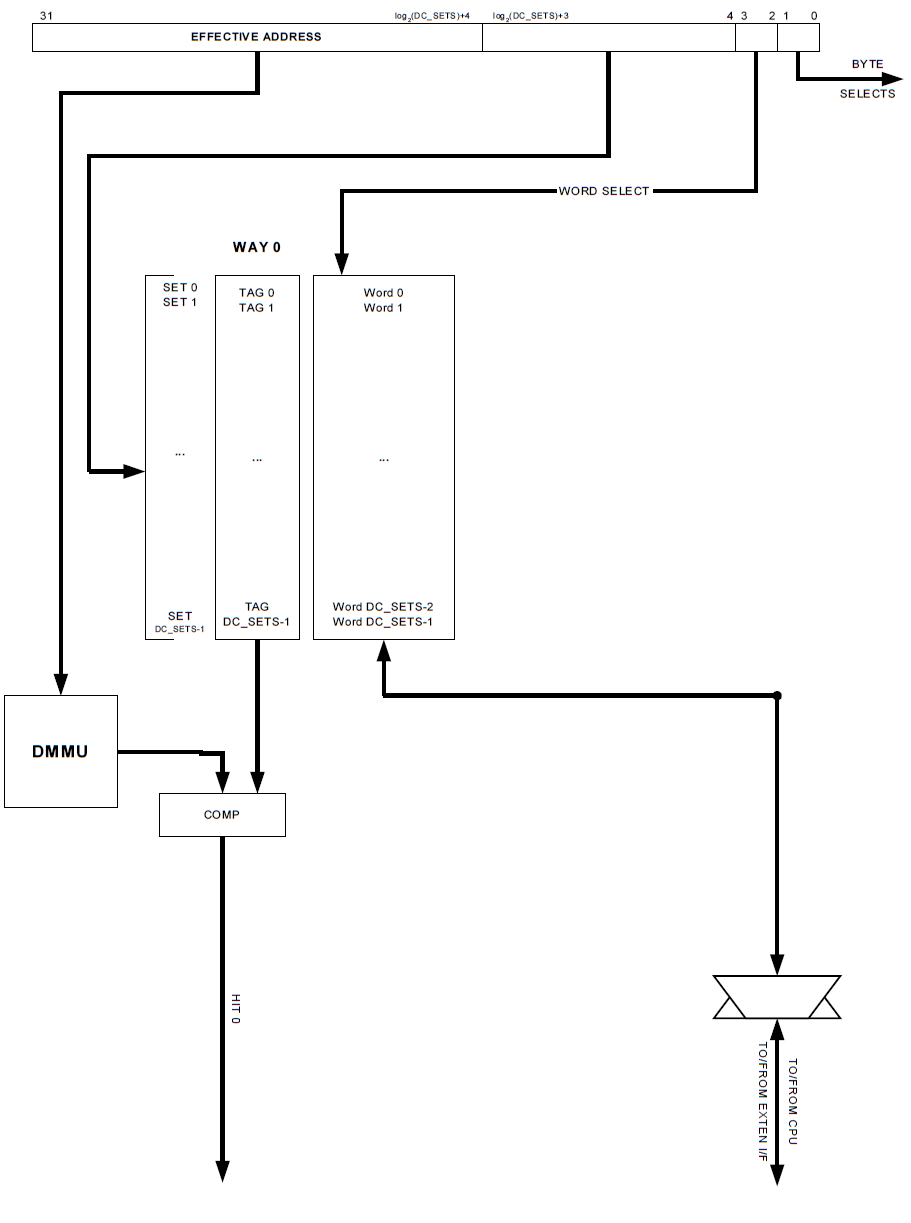
\includegraphics[bb=0 0 906 1228,scale=0.38]{./Images/data_cache.png}
 % data_cache.png: 906x1228 pixel, 72dpi, 31.96x43.32 cm, bb=0 0 906 1228
 \caption{Οργάνωση κρυφής μνήμης δεδομένων.}
\end{figure}
\vspace{0.7cm}

Κάθε γραμμή περιέχει τέσσερις συνεχόμενες λέξεις από τη μνήμη που έχουν φορτωθεί από μια 
οριοθετημένη γραμμή ως προς το μέγεθός της. Ως αποτέλεσμα, οι γραμμές της κρυφής μνήμης 
είναι ευθυγραμμισμένες με τα όρια της σελίδας.

\subsubsection{Κρυφή Μνήμη Εντολών}


Η προκαθορισμένες ρυθμίσεις για την κρυφή μνήμη εντολών για τον OR1200 είναι 8-KByte, 1-τρόπων πλήρους απεικόνισης (1-way direct-mapped),
οι οποίες επιτρέπουν στον πυρήνα ταχεία προσπέλαση στις εντολές. Παρόλα αυτά η κρυφή μνήμη μπορεί να παραμετροποιηθεί σύμφωνα με τον Πίνακα 2.7.
\setlength{\tabcolsep}{3em}
{%
\vspace{0.7cm}
\newcommand{\mc}[3]{\multicolumn{#1}{#2}{#3}}
\definecolor{tcA}{rgb}{1,1,0}
\begin{table}[h]
\begin{center}
\begin{tabular}{ |r|c|}
% use packages: color,colortbl
\hline
\rowcolor{tcA}
  & Direct mapped\\ \hline 
16B/line, 32 lines, 1 way & \mc{1}{c|}{512B}\\
16B/line, 256 lines, 1 way & \mc{1}{c|}{4KB}\\
16B/line, 512 lines, 1 way & \mc{1}{c|}{\textbf{8KB (default)}}\\
16B/line, 1024 lines, 1 way & \mc{1}{c|}{16KB}\\
32B/line, 1024 lines, 1 way & \mc{1}{c|}{32KB} \\ \hline
\end{tabular}
\end{center}
\caption{Ρυθμίσεις μεγέθους κρυφής μνήμης εντολών}
\end{table}

}%


Χαρακτηριστικά:


\begin{itemize}
 \item Η κρυφή μνήμη εντολών είναι ξεχωριστά υλοποιημένη από την κρυφή μνήμη δεδομένων (Harvard αρχιτεκτονική).
 \item Η κρυφή μνήμη εντολών χρησιμοποιεί τον αλγόριθμο "Λιγότερο Πρόσφατα Χρησιμοποιημένο" για την αντικατάσταση των πλαισίων.
 \item Ο κατάλογος της κρυφής μνήμης είναι φυσικά διευθυνσιοδοτημένος (physically addressed). Η ετικέτα της φυσικής διεύθυνσης είναι αποθηκευμένη στον κατάλογο της κρυφής μνήμης.
 \item Μπορεί να απενεργοποιηθεί ή να ακυρωθεί/ γράφοντας στους καταχωρητές ειδικού σκοπού της κρυφής μνήμης.
\end{itemize}



Κατά την αστοχία της κρυφής μνήμης η γραμμή της κρυφής μνήμης
γεμίζει ή με ριπές (burst) των 16-byte (default). Οι ριπές πραγματοποιούνται
σαν κρίσιμη-λέξη-πρώτα (critical-word-first) λειτουργία˙ η κρίσιμη γράφεται στην κρυφή μνήμη
και ταυτόχρονα προωθείται στην μονάδα αιτήσεων (requesting unit), έτσι μειώνονται οι καθυστερήσεις
που προκαλούνται από το γέμισμα της γραμμής. Η κρυφή μνήμη εντολών παρέχει αποθηκευτικό χώρο για τις
ετικέτες και εκτελεί συναρτήσεις αντικατάστασης γραμμών.
\newline

Η κρυφή μνήμη εντολών είναι στενά συνδεδεμένη με μια εξωτερική διεπαφή ώστε να επιτρέπει την αποδοτική
πρόσβαση στον ελεγκτή μνήμης.
\newline

Παράλληλα η κρυφή μνήμη εντολών προμηθεύει τις εντολές προς εκτέλεση διαμέσου
της διεπαφής των 32-bit της υπομονάδας προσκόμισης εντολών. Η υπομονάδα προσκόμισης εντολών
 παρέχει όλη την απαραίτητη λογική για
τον υπολογισμό της αποτελεσματικής διεύθυνσης (effective addresses).

\vspace{0.7cm}
\begin{figure}[h!]
 \centering
 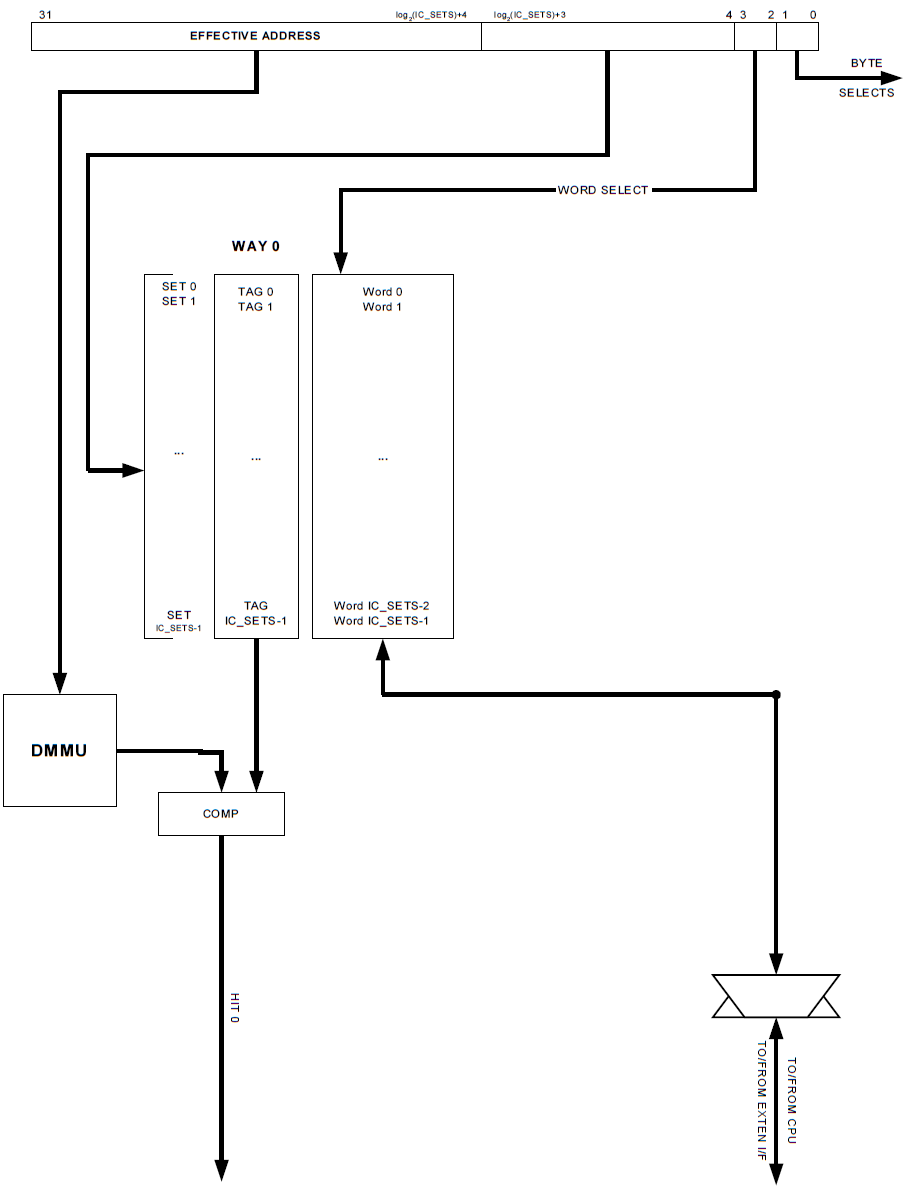
\includegraphics[bb=0 0 908 1201,scale=0.38]{./Images/instruction_cache.png}
 % instruction_cache.png: 908x1201 pixel, 72dpi, 42.37x32.03 cm, bb=0 0 1201 908
 \caption{Οργάνωση κρυφής μνήμης εντολών}
\end{figure}
\vspace{0.7cm}



Κάθε γραμμή περιέχει τέσσερις συνεχόμενες λέξεις από τη μνήμη που έχουν φορτωθεί από μια 
οριοθετημένη γραμμή ως προς το μέγεθός της. Ως αποτέλεσμα, οι γραμμές της κρυφής μνήμης 
είναι ευθυγραμμισμένες με τα όρια της σελίδας.

\subsubsection{Διαχείριση Μνήμης (MMU) Δεδομένων}

Η OR1200 υλοποιεί ένα εικονικό σύστημα διαχείρισης μνήμης (memomy management unit - MMU) 
που παρέχει προστασία κατά την πρόσβαση στην μνήμη και αποτελεσματική μετάφραση σε φυσικές
 διευθύνσεις. Η διακριτότητα της προστασίας είναι όπως ορίζεται από την αρχιτεκτονική 
OpenRISC 1000 8-Kbyte και 16-Mbyte σελίδες.

\setlength{\tabcolsep}{3em}
{%
\vspace{0.7cm}
\newcommand{\mc}[3]{\multicolumn{#1}{#2}{#3}}
\definecolor{tcA}{rgb}{1,1,0}
\begin{table}[h]
\begin{center}
\begin{tabular}{ |r|c|}
% use packages: color,colortbl
\hline
\rowcolor{tcA}
  & Direct mapped\\ \hline 
16 entries per way & \mc{1}{c|}{16 DTLB entries}\\
32 entries per way& \mc{1}{c|}{32 DTLB entries}\\
64 entries per way & \mc{1}{c|}{\textbf{64 DTLB entries (default)}}\\
128 entries per way & \mc{1}{c|}{128 DTLB entries} \\ \hline
\end{tabular}
\end{center}
\caption{Ρυθμίσεις Δεδομένων TLB (translation lookaside buffer)}
\end{table}
\vspace{0.7cm}
}%


Χαρακτηριστικά:

\begin{itemize}
 \item H MMU δεδομένων είναι ξεχωριστή από την MMU εντόλων.
 \item Το μέγεθός της σελίδας είναι 8-KByte.
 \item Ολοκληρωμένο σύστημα προστασίας σελίδας.
 \item Πλήρης απεικόνιση κατακερματισμού βασισμένο στον translation lookaside buffer (DTLB)
με προκαθορισμένο 1-τροπο συσχέτισης και τα παρακάτω χαρακτηριστικά:
	  \begin{itemize}
	      \item Παροχή εξαιρέσεων στην περίπτωση εξαιρέσεων και λαθών.
	      \item Software tablewalk.
	      \item Υψηλή απόδοση λόγο του κατακερματισμού.
	      \item Τροποποιήσιμο αριθμό καταχωρήσεων στο DLTB με προκαθορισμένες τις 64 καταχωρήσεις ανά τρόπο.
	  \end{itemize}
\end{itemize}

\newpage
\vspace{0.7cm}
\begin{figure}[h!]
 \centering
 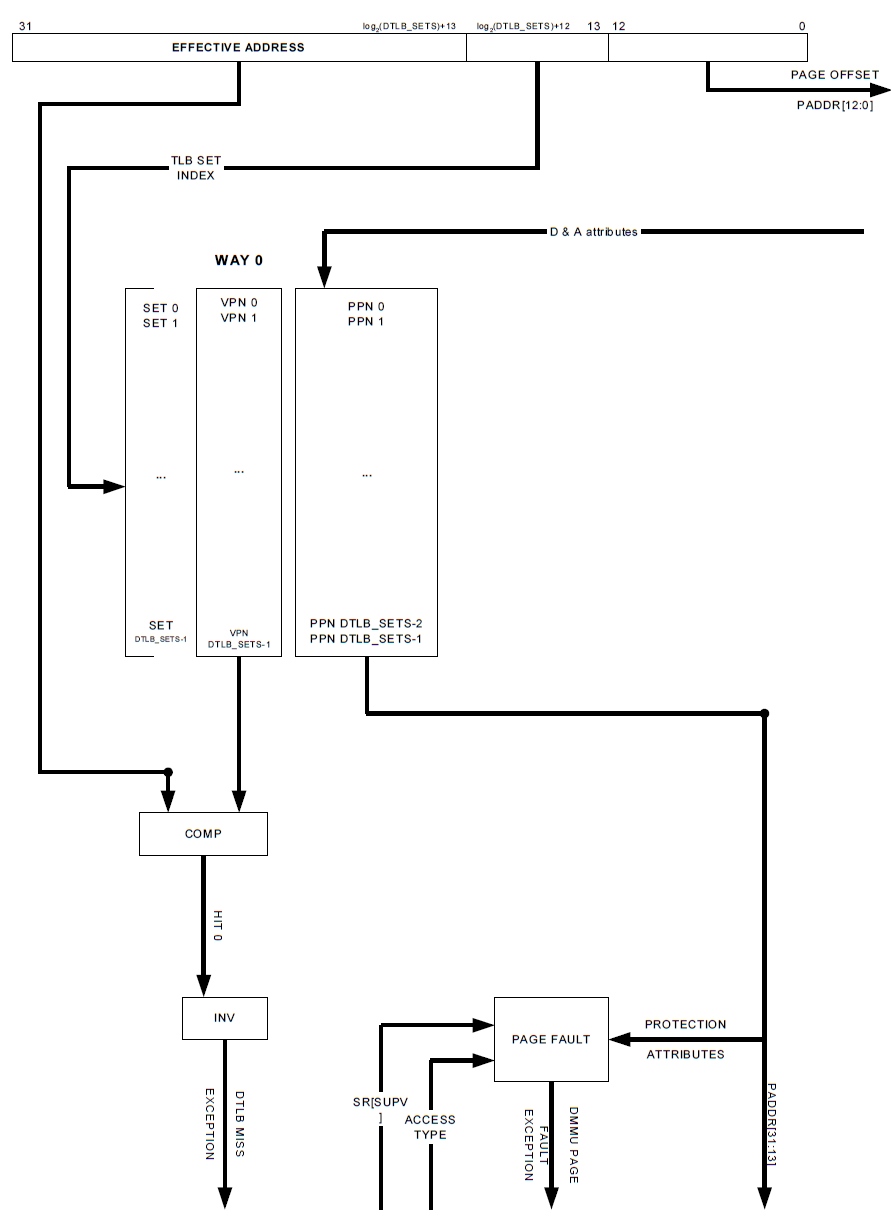
\includegraphics[bb=0 0 891 1229,scale=0.38]{./Images/data_MMU.png}
 % data_MMU.png: 891x1229 pixel, 72dpi, 31.43x43.36 cm, bb=0 0 891 1229
 \caption{Οργάνωση MMU δεδομένων.}
\end{figure}
\vspace{0.7cm}

Η υλοποίηση της MMU σε υλικό υποστηρίζει δύο-επιπέδων software tablewalk.
\vspace{0.7cm}
\begin{figure}[h!]
 \centering
 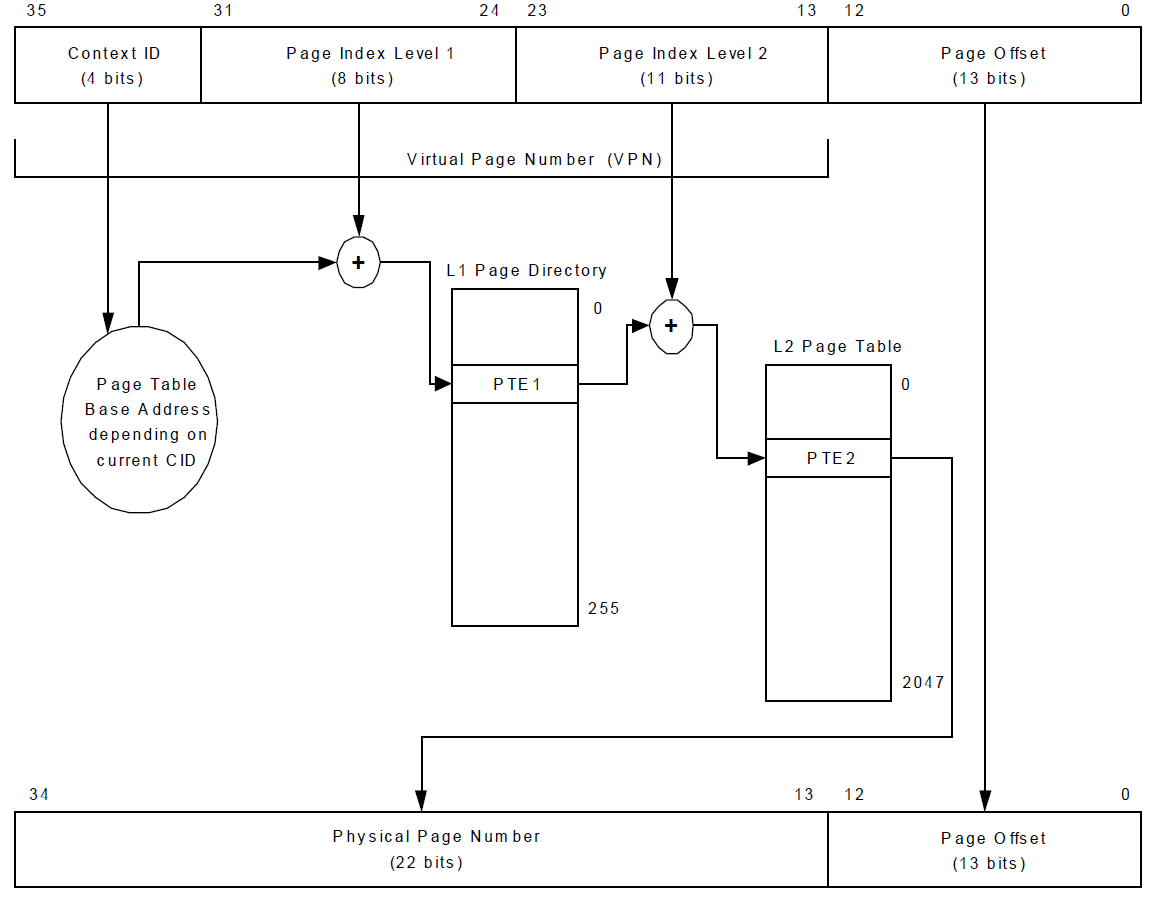
\includegraphics[bb=0 0 1158 899,scale=0.28]{./Images/DMMU_paging.png}
 % DMMU_paging.png: 1158x899 pixel, 72dpi, 40.85x31.71 cm, bb=0 0 1158 899
 \caption{Μηχανισμός μετάφρασης διευθύνσεων με την χρήση 2-επιπέδων πίνακα σελιδοποίησης.}
\end{figure}
\vspace{0.7cm}

\subsubsection{Διαχείριση Μνήμης (MMU) Εντολών}

Η OR1200 υλοποιεί ένα εικονικό σύστημα διαχείρισης μνήμης (memomy management unit - MMU) 
που παρέχει προστασία κατά την πρόσβαση στην μνήμη και αποτελεσματική μετάφραση σε φυσικές
 διευθύνσεις. Η διακριτότητα της προστασίας είναι όπως ορίζεται από την αρχιτεκτονική 
OpenRISC 1000 8-Kbyte και 16-Mbyte σελίδες.

\setlength{\tabcolsep}{3em}
{%
\vspace{0.7cm}
\newcommand{\mc}[3]{\multicolumn{#1}{#2}{#3}}
\definecolor{tcA}{rgb}{1,1,0}
\begin{table}[h]
\begin{center}
\begin{tabular}{ |r|c|}
% use packages: color,colortbl
\hline
\rowcolor{tcA}
  & Direct mapped\\ \hline 
16 entries per way & \mc{1}{c|}{16 ΙTLB entries}\\
32 entries per way& \mc{1}{c|}{32 ΙTLB entries}\\
64 entries per way & \mc{1}{c|}{\textbf{64 ΙTLB entries (default)}}\\
128 entries per way & \mc{1}{c|}{128 ΙTLB entries} \\ \hline
\end{tabular}
\end{center}
\caption{Ρυθμίσεις Εντολών TLB (translation lookaside buffer)}
\end{table}
\vspace{0.7cm}
}%


Χαρακτηριστικά:

\begin{itemize}
 \item H MMU εντόλων είναι ξεχωριστή από την MMU δεδομένων.
 \item Το μέγεθός της σελίδας είναι 8-KByte.
 \item Ολοκληρωμένο σύστημα προστασίας σελίδας.
 \item Πλήρης απεικόνιση κατακερματισμού βασισμένο στον translation lookaside buffer (ΙTLB)
με προκαθορισμένο 1-τρόπο συσχέτισης και τα παρακάτω χαρακτηριστικά:
	  \begin{itemize}
	      \item Παροχή εξαιρέσεων στην περίπτωση εξαιρέσεων και λαθών.
	      \item Software tablewalk.
	      \item Υψηλή απόδοση λόγο του κατακερματισμού.
	      \item Τροποποιήσιμο αριθμό καταχωρήσεων στο ILTB με προκαθορισμένες τις 64 καταχωρήσεις ανά τρόπο.
	  \end{itemize}
\end{itemize}

\newpage
\vspace{0.7cm}
\begin{figure}[h!]
 \centering
 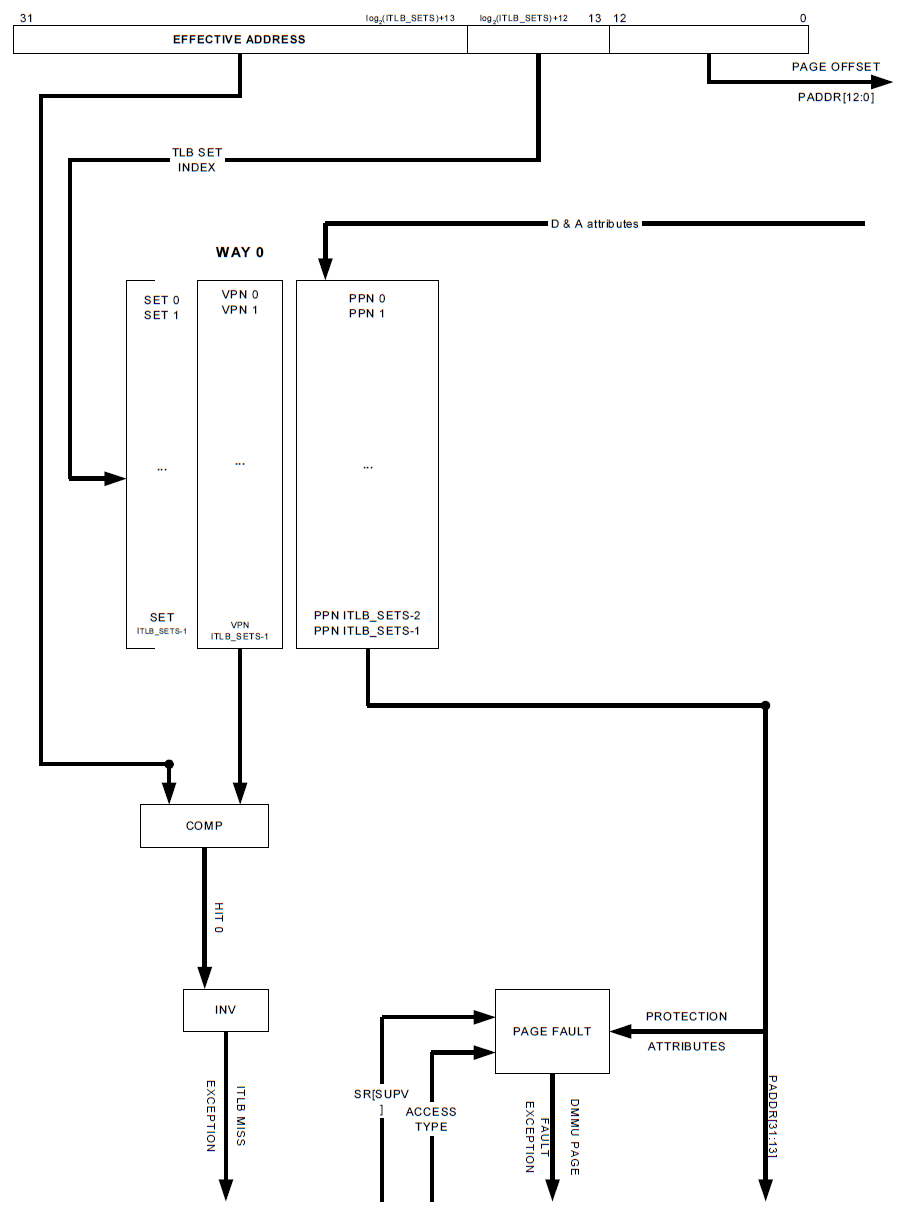
\includegraphics[bb=0 0 891 1229,scale=0.38]{./Images/instruction_MMU.png}
 % data_MMU.png: 891x1229 pixel, 72dpi, 31.43x43.36 cm, bb=0 0 891 1229
 \caption{Οργάνωση MMU εντολών.}
\end{figure}
\vspace{0.7cm}

Η υλοποίηση της MMU σε υλικό υποστηρίζει δύο-επιπέδων software tablewalk.

\vspace{0.7cm}
\begin{figure}[h!]
 \centering
 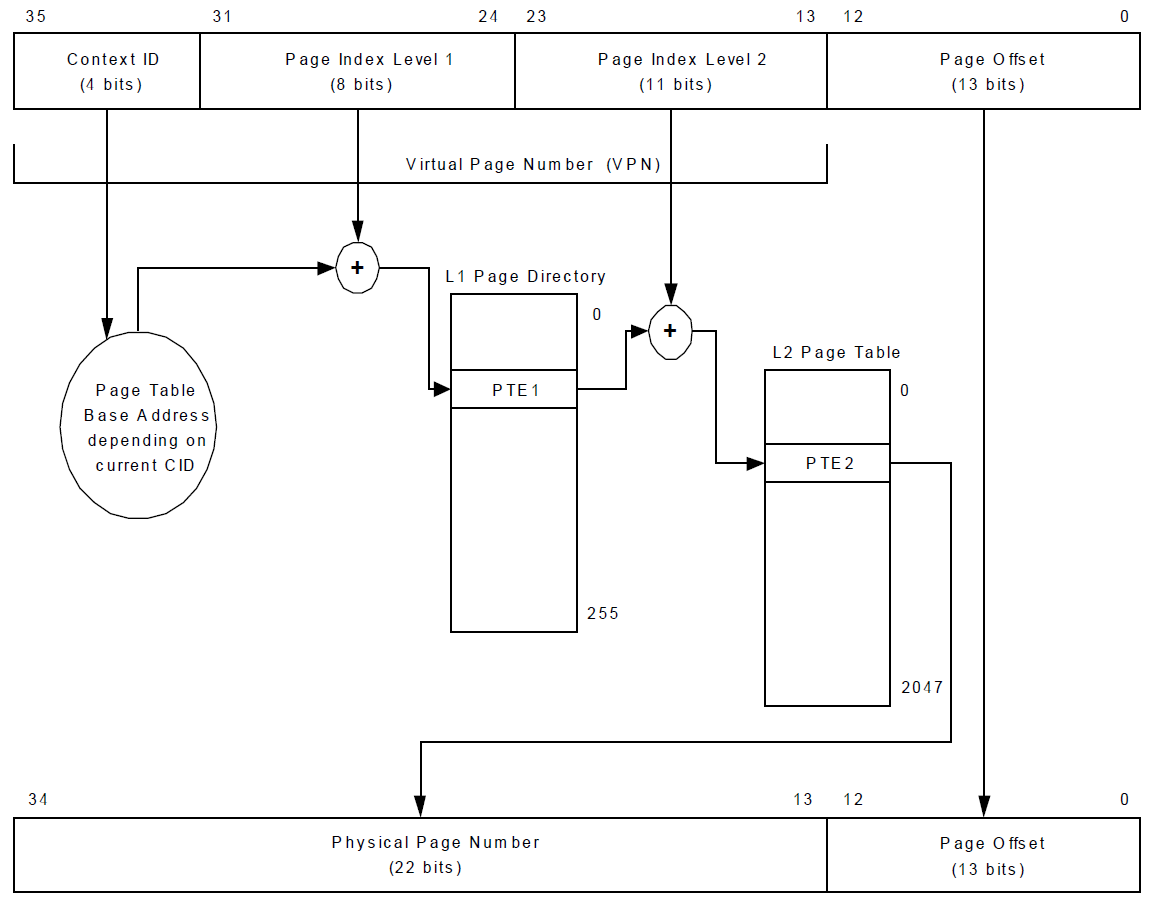
\includegraphics[bb=0 0 1158 899,scale=0.25]{./Images/IMMU_paging.png}
 % DMMU_paging.png: 1158x899 pixel, 72dpi, 40.85x31.71 cm, bb=0 0 1158 899
 \caption{Μηχανισμός μετάφρασης διευθύνσεων με την χρήση 2-επιπέδων πίνακα σελιδοποίησης.}
\end{figure}
\vspace{0.7cm}


\subsubsection{Προγραμματιζόμενος Ελεγκτής Διακοπών}

Ο ελεγκτής διακοπών (Interrupt controller) λαμβάνει διακοπές από εξωτερικές πηγές και τις
προωθεί ανάλογα με την προτεραιότητά τους (χαμηλή-υψηλή) σαν εξαιρέσεις (exception) στον
πυρήνα του επεξεργαστή.
\newline

Ο προγραμματιζόμενος ελεγκτής διακοπών έχει 32 σήματα εισόδου διακοπών και τρεις καταχωρητές ειδικού σκοπού, οι οποίοι είναι:
\begin{itemize}
 \item \underline{\emph{PICMR register:}} Αυτός ο καταχωρητής χρησιμοποιείται για να φιλτράρει (mask) τα 30 προγραμματιζόμενα σήματα διακοπών.
 \item \underline{\emph{PICPR register:}} Αυτός ο καταχωρητής χρησιμοποιείται για να αναθέτει προτεραιότητα (low-high) στα 30 προγραμματιζόμενα σήματα διακοπών.
 \item \underline{\emph{PICSR register:}} Αυτός ο καταχωρητής χρησιμοποιείται για να ελέγχει και να τροποποιεί την κατάσταση καθενός ξεχωριστά σήματος διακοπής ανάλογα με τον αν έχει εξυπηρετηθεί ή όχι.
\end{itemize}




Τα σήματα εισόδου διακοπών \emph{int0} και \emph{int1} είναι πάντα ενεργοποιημένα και συνδεδεμένα 
με την υψηλή και την χαμηλή προτεραιότητα εισόδου ​​αντίστοιχα, όπως φαίνεται και στο σχήμα 2.10.


\vspace{0.7cm}
\begin{figure}[h!]
 \centering
 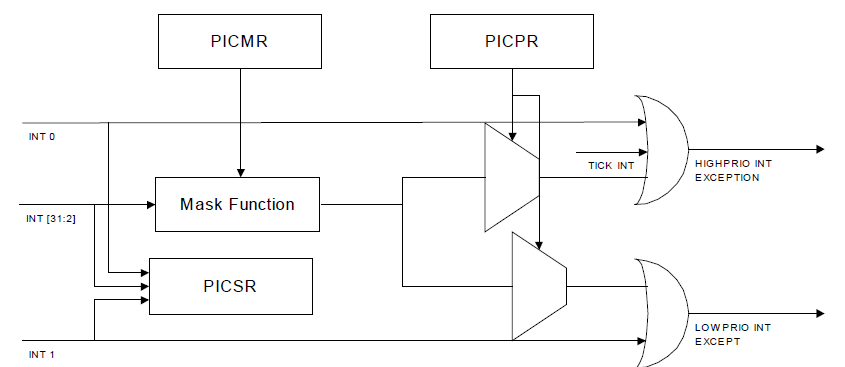
\includegraphics[bb=0 0 845 367,scale=0.38]{./Images/inter_controller.png}
 % inter_controller.png: 845x367 pixel, 72dpi, 29.81x12.95 cm, bb=0 0 845 367
 \caption{Μπλοκ διάγραμμα του ελεγκτή διακοπών.}
\end{figure}
\vspace{0.7cm}
\newpage
Όταν μια διακοπή προκαλείται σε ένα από τα τριάντα σήματα διακοπών (δηλαδή όταν το συγκεκριμένο σήμα-π.χ \emph{int14}- παίρνει τιμή στον καταχωρητή PICSR), τότε καμία νέα διακοπή δεν μπορεί να εξυπηρετηθεί στο ίδιο σήμα (\emph{int14}) μέχρι να καθαριστεί το δυαδικό ψηφίο που το αντιπροσωπεύει στον καταχωρητή PICSR.  Η συνήθης διαδικασία που ακολουθείται όταν μια διακοπή προκαλείται είναι η παρακάτω.
\begin{enumerate}
 \item Το περιφερειακό προσπαθεί να πάρει τον έλεγχο του επεξεργαστή ενεργοποιώντας το σήμα διακοπής που του έχει αντιστοιχιστεί. Αυτό έχει σαν αποτέλεσμα να πυροδοτείται εκείνη την στιγμή ο διαχειριστής διακοπών.
 \item Ο διαχειριστής διακοπών επεξεργάζεται την διακοπή.
 \item Ο διαχειριστής ενημερώνει το περιφερειακό ότι η διακοπή που προκάλεσε επεξεργάστηκε (συνήθως μέσω memory-mapped καταχωρητή).
 \item Το περιφερειακό αποσύρει την αίτηση που είχε κάνει.
 \item Ο διαχειριστής διακοπών καθαρίζει το αντίστοιχο δυαδικό ψηφίο στον PICSR καταχωρητή.
\end{enumerate}




\subsubsection{Tick Timer}

O επεξεργαστής OR1200 έχει υλοποιημένη λειτουργία χρονιστή (tick timer). Βασικά αυτός είναι
ένας χρονοδιακόπτης που χρονίζεται από το ρολόι του επεξεργαστή και χρησιμοποιείται από το
λειτουργικό σύστημα για ακριβείς μετρήσεις χρόνου και για τον χρονοπρογραμματισμό των διεργασιών τους
συστήματος.
\newline

Ο OR1200 ακολουθεί αυστηρά τον αρχιτεκτονικό ορισμό του χρονιστή όπου:

\begin{itemize}
 \item Μέγιστες μετρήσεις του χρονιστή $2^{32}$ κύκλους ρολογιού.
 \item Μέγιστη χρονική περίοδο, $2^{28}$ κύκλους ρολογιού μεταξύ διακοπών.
 \item Φιλτραρισμένο σήμα διακοπής χρονιστή (Maskable tick timer interrupt).
 \item Δυνατότητα επανεκκίνησης, μονής και συνεχούς μέτρησης.
\end{itemize}


\subsubsection{Διαχείριση Ενεργειακών Απαιτήσεων}

Για την βελτιστοποίηση της κατανάλωσης ενέργειας, ο OR1200 παρέχει καταστάσεις (mode)
χαμηλής ενεργειακής κατανάλωσης που μπορούν να χρησιμοποιηθούν ώστε δυναμικά να ενεργοποιούνται
και να απενεργοποιούνται ορισμένες εσωτερικές ενότητες (module).
\newline

Ο OR1200 έχει τρεις κύριες λειτουργίες για την ελαχιστοποίηση της κατανάλωσης ενέργειας:
\begin{itemize}
 \item Slow και Idle καταστάσεις (SW controlled clock freq reduction)
 \item Doze και Sleep καταστάσεις (interrupt wake-up)
\end{itemize}

\setlength{\tabcolsep}{1em}
\definecolor{tcA}{rgb}{1,1,0}
\begin{table}[h]
\begin{center}
\begin{tabular}{|l|l|}\hline
% use packages: color,colortbl
\rowcolor{tcA}
Power Minimization Feature & Approx Power Consumption Reduction\\\hline
Slow and Idle mode & 2x – 10x\\\hline
Doze mode & 100x\\\hline
Sleep mode & 200x\\\hline
Dynamic clock gating & N/A\\\hline
\end{tabular}
\end{center}
\caption{Καταστάσεις βελτιστοποίησης κατανάλωσης ενέργειας.}
\end{table}


Η κατάσταση Slow Down εκμεταλλεύεται τους low-power διαιρέτες από το εξωτερικό κύκλωμα 
παραγωγής ρολογιού ώστε να επιτυγχάνει πλήρης λειτουργικότητα αλλά σε χαμηλότερη συχνότητα, εξοικονομώντας έτσι ενέργεια.
\newline

Όταν το λογισμικό εκκινεί την κατάσταση Doze, τότε τα προγράμματα που τρέχουν στον επεξεργαστή
αναστέλλονται. Τα ρολόγια στις εσωτερικές ενότητες (modules) του επεξεργαστή απενεργοποιούνται 
εκτός του χρονιστή (tick timer). Ωστόσο οποιοδήποτε άλλο μπλόκ πάνω στο ολοκληρωμένο κύκλωμα
συνεχίζει να λειτουργεί κανονικά. Ο επεξεργαστής OR1200 θα φύγει από την κατάσταση doze και 
θα επανέλθει σε κανονική κατάσταση όταν κάποια διακοπή (interrupt) παρουσιαστεί.
\newline

Στην κατάσταση Sleep, όλες οι εσωτερικές μονάδες του OR1200 απενεργοποιούνται και τα 
ρολόγια οριοθετούνται (clocks gated). Προαιρετικά (ανάλογα με την υλοποίηση) μπορεί να χαμηλωθεί 
η παροχή της τάσης στον πυρήνα του OR1200. Ο επεξεργαστής OR1200 θα φύγει από την κατάσταση doze και 
θα επανέλθει σε κανονική κατάσταση όταν κάποια διακοπή (interrupt) παρουσιαστεί.
\newline

Η λειτουργία Dynamic Clock gating δεν υποστηρίζεται προς το παρών από τον OR1200. 

\subsubsection{Μονάδα Αποσφαλμάτωσης}

Η μονάδα αποσφαλμάτωσης βοηθάει τους προγραμματιστές λογισμικού διορθώσουν λάθη στο σύστημα
τους. Παρέχει την βασική βοήθεια για αποσφαλμάτωση, χωρίς να παρέχει όμως προηγμένη τεχνολογία
σύμφωνα με την αρχιτεκτονική του OpenRISC 1000 όπως watchpoints, breakpoints και πρόγραμμα
ελέγχου της ροής των καταχωρητών ελέγχου.

\vspace{0.7cm}
\begin{figure}[h!]
 \centering
 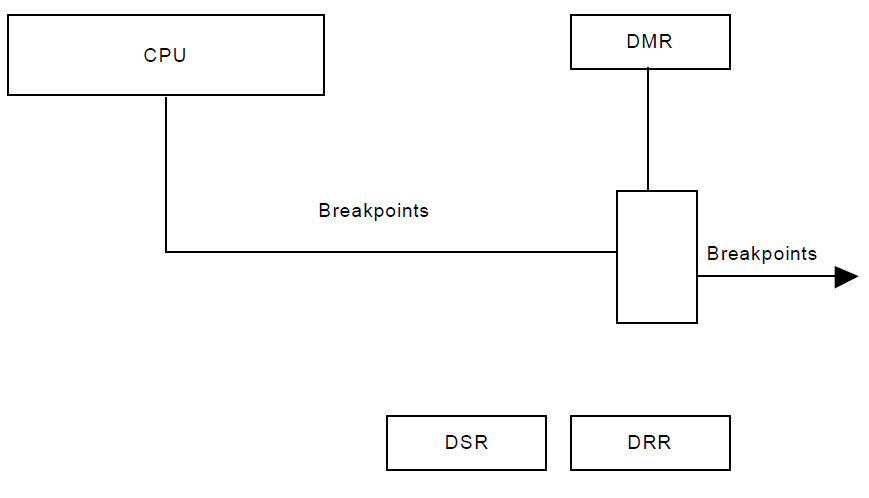
\includegraphics[bb=0 0 869 498,scale=0.38]{./Images/debug_unit.png}
 % debug_unit.png: 869x498 pixel, 72dpi, 30.66x17.57 cm, bb=0 0 869 498
 \caption{Μπλόκ διάγραμμα μονάδας αποσφαλμάτωσης.}
\end{figure}
\vspace{0.7cm}

\subsubsection{Σήματα Χρονισμού και Επανεκκίνησης}

O πυρήνας του OR1200 χρησιμοποιεί ένα ρολόι για τον χρονισμό κάθε μιας διεπαφή του διαύλου
επικοινωνίας Wishbone τόσο για τα δεδομένα όσο και για τις εντολές. Το σήμα ρολογιού \emph{clk\_cpu}
χρονίζει οτιδήποτε βρίσκεται μέσα στην διεπαφή του διαύλου Wishbone. Η διεπαφή διαύλου δεδομένων
Wishbone χρονίζεται από το σήμα \emph{dwd\_clk\_i}, ενώ των εντολών με το σήμα \emph{iwd\_clk\_i}.
\newline

O επεξεργαστής OR1200 παρέχει ένα ασύγχρονο σήμα επανεκκίνησης του συστήματος (asynchronous reset signal)
, \emph{rst}. Όταν αυτό σήμα είναι ενεργοποιημένο τότε αμέσως επαναφέρει (resets) όλα τα 
flip-flops μέσα στον OR1200. Όταν είναι απενεργοποιημένο τότε ο επεξεργαστής λειτουργεί κανονικά.

\subsubsection{Δίαυλος επικοινωνίας Wishbone}

Δύο διεπαφές Wishbone του επεξεργαστή OR1200 συνδέουν τον πυρήνα με τα περιφερειακά και το
εξωτερικό υποσύστημα μνήμης. Αυτές είναι συμβατές το WISHBONE SoC Interconnection specification Rev. B3.
Η υλοποίηση παρέχει ένα δίαυλο επικοινωνίας πλάτους 32 bit χωρίς να υποστηρίζει άλλα πλάτη.

\newpage
\subsection{I/O Θύρες}

Ο επεξεργαστής OR1200 προσφέρει τις παρακάτω διεπαφές για σύνδεση με εξωτερικές λειτουργίες.
\begin{itemize}
 \item Instruction and data WISHBONE host interfaces
 \item Power management interface
 \item Development interface
 \item Interrupts interface
\end{itemize}
\vspace{0.7cm}
\begin{figure}[h!]
 \centering
 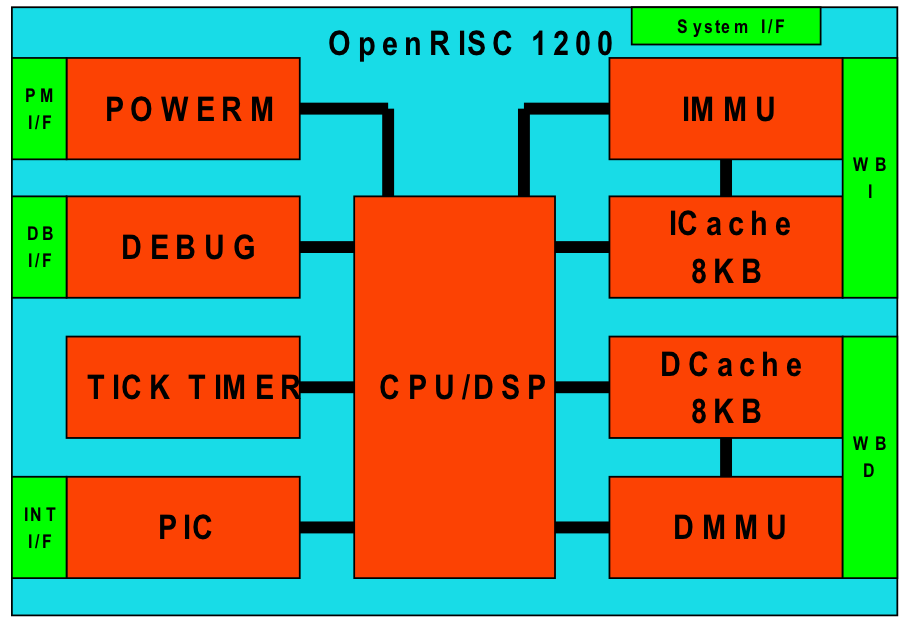
\includegraphics[bb=0 0 905 625,scale=0.3]{/home/federico/Documents/Kile/Diploma/Images/or1200.png}
 % or1200.png: 905x625 pixel, 72dpi, 31.93x22.05 cm, bb=0 0 905 625
 \caption{Core's Interfaces}
\end{figure}
\vspace{0.7cm}
Σε αυτή την ενότητα θα αναλυθούν όλες οι διεπαφές που προσφέρει ο επεξεργαστής OR1200 εκτός από την διεπαφές δεδομένων και εντολών Wishbone που θα περιγραφούν στην κεφάλαιο 4 στην ενότητα 4.3.

\subsubsection{Διεπαφή Συστήματος (System I/F)}

Με την διεπαφή συστήματος συνδέονται στο επεξεργαστή OR1200 σήματα όπως το reset, το ρολόι (clock) και τα υπόλοιπα που φαίνονται στον παρακάτω πίνακα.
\newpage
{%
\vspace{0.7cm}
\renewcommand{\arraystretch}{1.2}
\setlength{\tabcolsep}{0.3em}
\newcommand{\mc}[3]{\multicolumn{#1}{#2}{#3}}
\definecolor{tcA}{rgb}{1,1,0}
\begin{table}[h]
\begin{center}
\begin{tabular}{|l|l|l|l|}
% use packages: color,colortbl
\hline
\rowcolor{tcA}
Port & Width & Direction & Description\\\hline
Rst & 1 & Input &Asynchronous reset\\\hline
clk\_cpu & 1 & Input & Main clock input to the RISC\\\hline
clk\_dc & 1 & Input &Data cache clock\\\hline
clk\_ic & 1 & Input & Instruction cache clock\\\hline
clk\_dmmu & 1 & Input & Data MMU clock\\\hline
clk\_immu & 1 & Input & Instruction MMU clock \\\hline
clk\_tt & 1 & Input & Tick timer clock\\\hline
\end{tabular}
\end{center}
\caption{Σήματα διεπαφής συστήματος.}
\end{table}
\vspace{0.7cm}
}%

\subsubsection{Διεπαφή Ανάπτυξης (Development DB I/F)}

H διεπαφή ανάπτυξης συνδέει την εξωτερική θύρα εντοπισμού σφαλμάτων με την εσωτερική μονάδα αποσφαλμάτωσης του επεξεργαστή OR1200. Η μονάδα αποσφαλμάτωσης όπως αναφέρθηκε και παραπάνω επιτρέπει τον έλεγχο της εκτέλεση προγραμμάτων μέσα στον RISC επεξεργαστή, των καθορισμό breakpoints και watchpoints όπως και την ροή δεδομένων και εντολών. Στον παρακάτω πίνακα φαίνονται τα σήματα που παρέχει αυτή η διεπαφή.

{%
\vspace{0.7cm}
\renewcommand{\arraystretch}{1.2}
\setlength{\tabcolsep}{0.3em}
\newcommand{\mc}[3]{\multicolumn{#1}{#2}{#3}}
\definecolor{tcA}{rgb}{1,1,0}
\begin{table}[h]
\begin{center}
\begin{tabular}{|l|l|l|l|}
% use packages: color,colortbl
\hline
\rowcolor{tcA}
Port & Width & Direction & Description\\\hline
dbg\_dat\_o & 32 & Output & Transfer of data from RISC to external development interface\\\hline
dbg\_dat\_i & 32 & Input & Transfer of data from external development interface to RISC\\\hline
dbg\_adr\_i & 32 & Input & Address of special-purpose register to be read or written\\\hline
dbg\_op\_I & 3 & Input & Operation select for development interface\\\hline
dbg\_lss\_o & 4 & Output & Status of load/store unit\\\hline
dbg\_is\_o & 2 & Output & Status of instruction fetch unit\\\hline
dbg\_wp\_o & 11 & Output & Status of watchpoints\\\hline
dbg\_bp\_o & 1 & Output & Status of the breakpoint\\\hline
dbg\_stall\_i & 1 & Input & Stalls RISC CPU core\\\hline
dbg\_ewt\_i & 1 & Input & External watchpoint trigger\\\hline
\end{tabular}
\end{center}
\caption{Development Interface}
\end{table}
\vspace{0.7cm}
}%

\subsubsection{Διεπαφή Ελέγχου Ενέργειας (Power Management I/F)}

H διεπαφή ελέγχου ενέργειας (Power Management Interface) παρέχει σήματα που συνδέουν τον επεξεργαστή OR1200 με εξωτερικές πηγές ενέργειας. Οι εξωτερικές πηγές ενέργειας χρειάζονται για την υλοποίηση συναρτήσεων των οποίων η τεχνολογία δεν επιτρέπει την υλοποίηση τους μέσα στον πυρήνα. Στον παρακάτω πίνακα φαίνονται τα σήματα που παρέχει αυτή η διεπαφή.
{%
\vspace{0.7cm}
\renewcommand{\arraystretch}{1.2}
\setlength{\tabcolsep}{0.3em}
\newcommand{\mc}[3]{\multicolumn{#1}{#2}{#3}}
\definecolor{tcA}{rgb}{1,1,0}
\begin{table}[h]
\begin{center}
\begin{tabular}{|l|l|l|l|p{6 cm}|}
% use packages: color,colortbl
\hline
\rowcolor{tcA}
Port & Width & Direction  & Generation & Description\\\hline
pm\_clksd & 4 & Output & Static (in SW) & Slow down outputs that control reduction of RISC clock frequency\\\hline
pm\_cpustall & 1 & Input & - & Synchronous stall of the RISC’s CPU core\\\hline
pm\_dc\_gate & 1 & Output & Dynamic (in HW) & Gating of data cache clock\\\hline
pm\_ic\_gate & 1 & Output & Dynamic (in HW) & Gating of instruction cache clock\\\hline
pm\_dmmu\_gate & 1 & Output & Dynamic (in HW) & Gating of data MMU clock\\\hline
pm\_immu\_gate & 1 & Output & Dynamic (in HW) & Gating of instruction MMU clock\\\hline
pm\_tt\_gate & 1 & Output & Dynamic (in HW) & Gating of tick timer clock\\\hline
pm\_cpu\_gate & 1 & Output & Static (in SW) & Gating of main CPU clock\\\hline
pm\_wakeup & 1 & Output & Dynamic (in HW) &  Activate all clocks\\\hline
pm\_lvolt & 1 & Output & Static (in SW) & Lower voltage\\\hline
\end{tabular}
\end{center}
\caption{Σήματα διεπαφής ελέγχου ενέργειας}
\end{table}
\vspace{0.7cm}
}%

\subsubsection{Διεπαφή Διακοπών (Interrupt I/F)}

H διεπαφή Διακοπών (Interrupt interface) έχει σαν εισόδους τις διακοπές που προκαλούν οι εξωτερικές περιφερειακές μονάδες και τις καθοδηγούν εσωτερικά στον επεξεργαστή για να τις επεξεργαστή. Όλες οι διακοπές δημιουργούνται στην θετική ακμοπυροδότηση του κεντρικού ρολογιού του RISC επεξεργαστή. Στον παρακάτω πίνακα φαίνονται τα σήματα που παρέχει αυτή η διεπαφή.

{%
\vspace{0.7cm}
\renewcommand{\arraystretch}{1.2}
\setlength{\tabcolsep}{0.3em}
\newcommand{\mc}[3]{\multicolumn{#1}{#2}{#3}}
\definecolor{tcA}{rgb}{1,1,0}
\begin{table}[h]
\begin{center}
\begin{tabular}{|l|l|l|l|}
% use packages: color,colortbl
\hline
\rowcolor{tcA}
Port & Width & Direction  & Description\\\hline
pic\_ints & PIC\_INTS & Input & External interrupts\\\hline
\end{tabular}
\end{center}
\caption{Σήματα διεπαφής διακοπών}
\end{table}
\vspace{0.7cm}
}%
\newpage
\subsection{Παραμετροποίηση Επεξεργαστή}

Σε αυτή την ενότητα θα γίνει αναφορά στα χαρακτηριστικά του επεξεργαστή που μπορούν να παραμετροποιηθούν σε επίπεδο υλικού από τον χρήστη.
Στο παρακάτω πίνακα φαίνονται ποια είναι αυτά τα χαρακτηριστικά και ποιες οι αντίστοιχες μεταβλητές τους.
{%
\renewcommand{\arraystretch}{1.2}
\setlength{\tabcolsep}{0.3em}
\newcommand{\mc}[3]{\multicolumn{#1}{#2}{#3}}
\definecolor{tcA}{rgb}{1,1,0}
\begin{table}[h]
\begin{center}
\begin{tabular}{|l|l|l|l|}
% use packages: color,colortbl
\hline
\rowcolor{tcA}
Variable Name & Range & Default & Description\\\hline
EADDR\_WIDTH & 32 & 32 & Effective address width\\\hline
VADDR\_WIDTH & 32 & 32 & Virtual address width\\\hline
PADDR\_WIDTH & 24-36 & 32 & Physical address width\\\hline
DATA\_WIDTH & 32 & 32 & Data width / Operation width\\\hline
 &  &  & \\\hline
DC\_IMPL & 0-1 & 1 & Data cache implementation\\\hline
DC\_SETS & 256-1024 & 512 & Data cache number of sets\\\hline
DC\_WAYS & 1 & 1 & Data cache number of ways\\\hline
DC\_LINE & 16-32 & 16 & Data cache line size\\\hline
 &  &  & \\\hline
IC\_IMPL & 0-1 & 1 & Instruction cache implementation\\\hline
IC\_SETS & 32-1024 & 512 & Instruction cache number of sets\\\hline
IC\_WAYS & 1 & 1 & Instruction cache number of ways\\\hline
IC\_LINE & 16-32 & 16 & Instruction cache line size in bytes\\\hline
 &  &  & \\\hline
DMMU\_IMPL & 0-1 & 1 & Data MMU implementation\\\hline
DTLB\_SETS & 64 & 64 & Data TLB number of sets\\\hline
DTLB\_WAYS & 1 & 1 & Data TLB number of ways\\\hline
 &  &  & \\\hline
IMMU\_IMPL & 0-1 & 1 & Instruction MMU implementation\\\hline
ITLB\_SETS & 64 & 64 & Instruction TLB number of sets\\\hline
ITLB\_WAYS & 1 & 1 & Instruction TLB number of ways\\\hline
 &  &  & \\\hline
PIC\_INTS & 2 – 32 & 20 & Number of interrupt inputs\\\hline
\end{tabular}
\end{center}
\caption{Παραμετροποίηση Υλικού.}
\end{table}
}%





\newpage
\newpage

\section{OR1200 Προσομοίωση}

\subsection{Περιβάλλον Προσομοίωσης}
Υπάρχουν δύο περιβάλλοντα με τα οποία γίνετε η προσομοίωση του OR1200 επεξεργαστή.
Το πρώτο χρησιμοποιεί τον OpenRISC αρχιτεκτονικό προσομοιωτή \emph{or1ksim} και 
το δεύτερο χρησιμοποιεί τον \emph{NC-Verilog} προσομοιωτή που κάνει προσομοίωση με βάση
το υλικό (hardware based simulation). Στο πρώτο περιβάλλον γίνετε η επαλήθευση
της λειτουργικότητας των benchmarks και στο δεύτερο προσομοιώνεται η ουσιαστική
λειτουργία του OR1200 σε επίπεδο υλικού με βάση το benchmark που εκτελέσαμε.\newline


Η συνολική ροή της προσομοίωσης παρουσιάζεται στο Σχήμα 3.1. Τα benchmarks είναι 
είτε .C αρχεία είτε .S αρχεία. Αυτά τα αρχεία, αρχικά γίνονται cross-compiled
 χρησιμοποιώντας την εντολή or32-uclinux-gcc και παράγουν ένα .O object αρχείο. 
Το object αρχείο μετά μετατρέπεται σε ενα .OR32 εκτελέσιμο αρχείο χρησιμοποιώντας
την συνδετική εντολή or32-uclinux-ld. Αυτό το εκτελέσιμο αρχείο χρησιμοποιείται
από τον or1k αρχιτεκτονικό εξομοιωτή. Περαιτέρω το αρχείο .OR32 μετατρέπεται σε
δυαδικό (binary) αρχείο χρησιμοποιώντας την εντολή or32-uclinux-objcopy. Στο τέλος
δημιουργείται ένα .HEX αρχείο χρησιμοποιώντας τον binary to hex μετατροπέα
 bin2hex. Το παραγόμενο αρχείο .HEX φορτώνεται στην flash μνημη του RTL κώδικα
του OR1200 επεξεργαστή και μετά γινετε η προσομοίωση με βάση το υλικό.

\vspace{0.7cm}
\begin{figure}[h!]
 \centering
 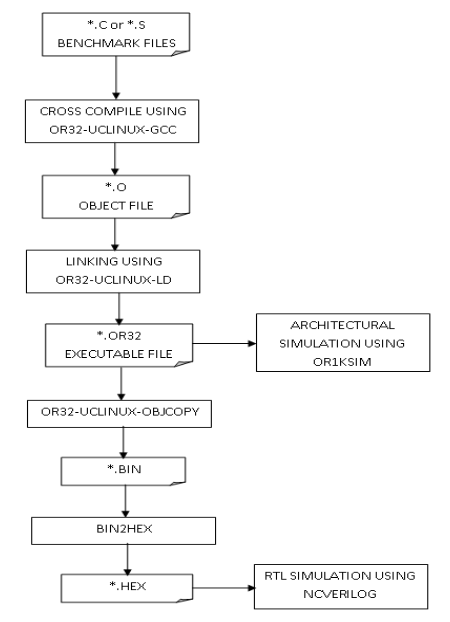
\includegraphics[bb=0 0 450 622,scale=0.5]{/home/federico/Documents/Kile/Diploma/Images/overall_flow.png}
 % overall_flow.png: 450x622 pixel, 72dpi, 15.88x21.94 cm, bb=0 0 450 622
 \caption{Συνολική ροή προσομοίωσης.}
\end{figure}
\vspace{0.7cm}
\newpage

Η συνολική ροή της προσομοίωσης ελέγχετε από το Makefile που παρέχεται από το Opencores μαζί με το πακέτο\footnote{Για την δομή των αρχείων σε αυτό το πακέτο δείτε την ενότητα 3.3} που περιέχει το επεξεργαστή OR1200. Το συγκεκριμένο Makefile δημιουργεί τα απαραίτητα αρχεία όπως περιγράφηκαν παραπάνω (Σχήμα 3.1) και τα οδηγεί τόσο στον αρχιτεκτονικό προσομοιωτή όσο και στον προσομοιωτή υλικού\footnote{Το Makefile τροποιήθηκε όπως φαίνεται στην υπο-ενότητα 3.2.2 για να υποστηρίζει τον προσομοιωτή υλικού NcVerilog} ώστε να γίνει η προσομοίωση. 

\newpage


\subsection{Εγκατάσταση Αλυσίδας Προσομοίωσης}
Σε αυτό το σημείο θα παρουσιάσουμε τον τρόπο με τον οποίο εγκαταστάθηκαν τα κατάλληλα προγράμματα με τα οποία γίνετε η προσομοίωση του επεξεργαστή OR1200 τόσο σε επίπεδο λογισμικού όσο και σε επίπεδο υλικού.
\newline
 Να σημειωθεί ότι παρόλο που ακολουθήθηκε ένας καθολικός τρόπος εγκατάστασης τέτοιων προγραμμάτων έγιναν αρκετές παραμετροποιήσεις
ώστε να μην επηρεαστεί η σωστή λειτουργία άλλων προγραμμάτων που είναι εγκατεστημένα στο εργαστήριο μικροηλεκτρονικής. Στο Σχήμα 3.2 φαίνεται η βασική διαδικασία που ακολουθήθηκε.

\vspace{0.7cm}
\begin{figure}[h!]
 \centering
 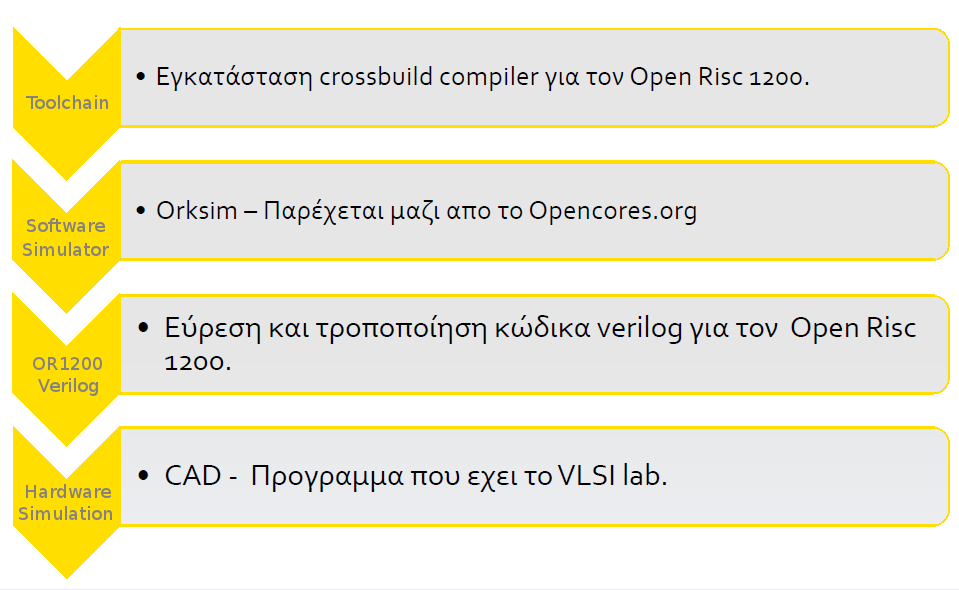
\includegraphics[bb=0 0 959 590,scale=0.35]{./Images/toolchain.png}
 % toolchain.png: 959x590 pixel, 72dpi, 33.83x20.81 cm, bb=0 0 959 590
 \caption{Διαδικασία Εγκατάστασης Προγραμμάτων}
\end{figure}
\vspace{0.7cm}
\newpage


\subsubsection{Εγκατάσταση Αρχιτεκτονικού Προσομοιωτή - Or1ksim}

Ο αρχιτεκτονικός προσομοιωτής ουσιαστικά είναι ένας τροποποιημένος gcc compiler που συνυπάρχει παράλληλα (crossbuild) με τον gcc compiler του συστήματος και βοηθά στην εκτέλεση αρχείων κώδικα assembly του επεξεργαστή Open Risc 1200.
\newline

Η διαδικασία που ακολουθήθηκε είναι η παρακάτω:
\begin{enumerate}
 \item Κατέβασμα του απαραίτητου script από το www.opencores.org που θα εγκαταστήσει τα απαραίτητα πακέτα για την σωστή λειτουργία του προσομοιωτή.
 \item Αλλαγές στο script για την εγκατάσταση των πακέτων σε τέτοιο σημείο στο σύστημά μας ώστε να μπορούν να το χρησιμοποιούν όλοι οι χρήστες του εργαστηρίου.
 \item Εκτέλεση του script σε terminal.
\end{enumerate}


Στο Σχήμα 3.3 φαίνεται ακριβώς η παραμετροποίηση που έγινε και το πως εκτελέστηκαν τα παραπάνω βήματα.
\vspace{0.7cm}
\begin{figure}[h!]
 \centering
 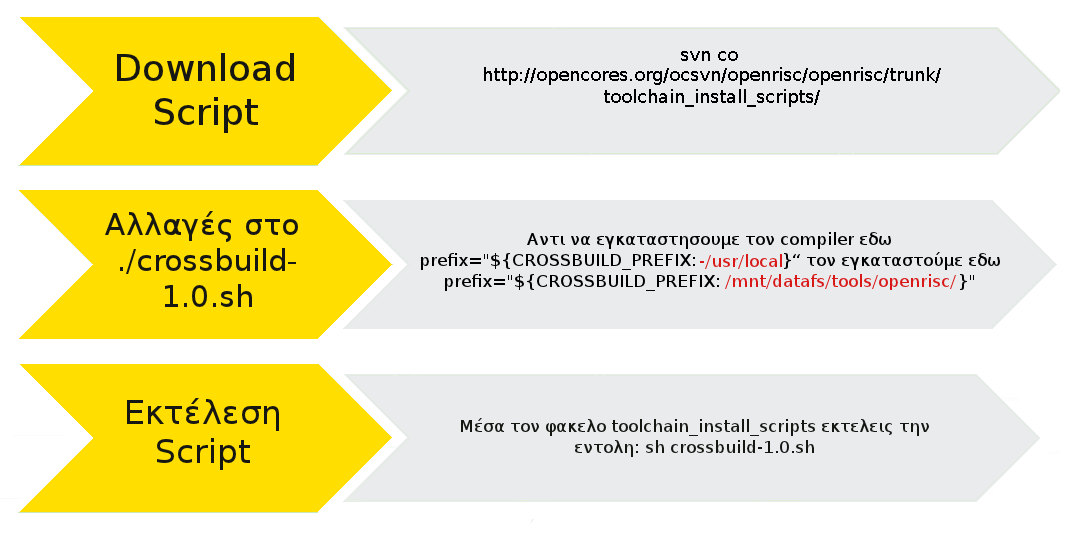
\includegraphics[bb=0 0 1065 546,scale=0.31]{./Images/or1ksim.png}
 % or1ksim.png: 1065x546 pixel, 72dpi, 37.57x19.26 cm, bb=0 0 1065 546
 \caption{Εντολές εγκατάστης του Or1ksim.}
\end{figure}
\vspace{0.7cm}

\newpage

Σε αυτό το σημείο είναι απαραίτητο να σημειωθεί ότι η εκτέλεση του δεύτερου βήματος ήταν από τις πιο χρονοβόρες διαδικασίες που έγιναν για την εκπόνηση αυτής της διπλωματικής εργασίας. 
Οι λόγοι είναι οι παρακάτω:
\begin{enumerate}
 \item Για την εκτέλεση του script που θα εγκαθιστούσε τον τροποποιημένο GCC compiler για τον OR1200 έπρεπε να αναβαθμιστεί ο υπάρχων GCC compiler και αρκετές άλλες βιβλιοθήκες ώστε να υποστηρίζει στην εκτέλεση κάποιων εσωτερικών εντολών του script. 
 \item Ο τροποποιημένος GCC compiler θα έπρεπε να λειτουργεί αρμονικά με τον αναβαθμισμένο GCC compiler του συστήματος του εργαστηρίου μικροηλεκτρονικής.
\end{enumerate}

Οι παραπάνω λόγοι αποτελούσαν προβλήματα κατά το στάδιο της εγκατάστασης του αρχιτεκτονικού προσομοιωτή Or1ksim επειδή η εγκατάσταση του έπρεπε να γίνει σε ένα υπάρχων υπολογιστικό σύστημα (του εργαστηρίου μικροηλεκτρονικής) και όχι σε ένα καινούργιο σύστημα. Αυτό είχε σαν συνέπεια να έπρεπε να διατηρηθεί η συμβατότητα των καινούργιων προγραμμάτων με τα προγράμματα που ήταν ήδη εγκατεστημένα στο εργαστήριο και χρησιμοποιούνταν για άλλους σκοπούς. Αυτό αντιμετωπίστηκε με την χρήση της μεθόδου trial and error όπως παρουσιάζεται στο Σχήμα 3.4 παρακάτω.

\vspace{0.7cm}
\begin{figure}[h!]
 \centering
 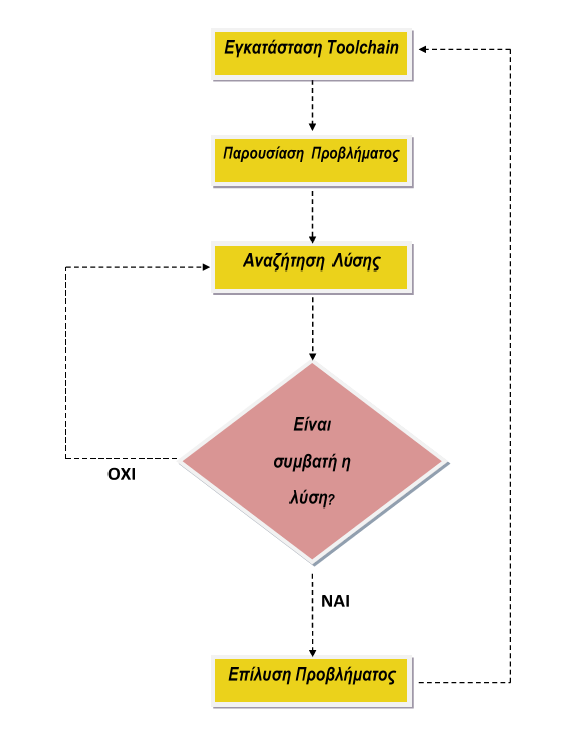
\includegraphics[bb=0 0 586 741,scale=0.4]{./Images/trial_and_error.png}
 % trial_and_error.png: 586x741 pixel, 72dpi, 20.67x26.14 cm, bb=0 0 586 741
 \caption{Trial and Error Method}
\end{figure}
\vspace{0.7cm}
\newpage


\subsubsection{Προσομοιωτής Υλικού NcVerilog}

Όπως αναφέρθηκε και στην ενότητα 3.1 η συνολική ροή της προσομοίωσης ελέγχεται από το Makefile που βρίσκεται στο \emph{./sim/bin/} στον φάκελο που περιέχει τον επεξεργαστή OR1200. To Makefile που παρέχει ελεύθερα το Opencores έχει υλοποιηθεί με τέτοιο τρόπο ώστε στο στάδιο της προσομοίωσης υλικού να δίνει τον έλεγχο είτε στο ICARUS\footnote{Προσομοιωτής υλικού από τον Stephen Williams. Διανέμεται ελεύθερα - Open source programm.} είτε στο Modelsim\footnote{Προσομοιωτής υλικού από την εταιρεία Mentor Graphics. Δεν διανέμεται ελεύθερα.}.

Ο προσομοιωτής υλικού που είναι εγκατεστημένος στο εργαστήριο μικροηλεκτρονικής και χρησιμοποιείται για ακαδημαϊκούς σκοπούς είναι ο NcVerilog της εταιρείας Cadence Design Systems που υποστηρίζει γλώσσες περιγραφής υλίκου (HDL) όπως η Verilog και η VHDL. 
\newline

Όπως γίνετε εύκολα αντιληπτό από τα παραπάνω για να χρησιμοποιηθεί ο NcVerilog προσομοιωτής έπρεπε να τροποποιηθεί το Makefile με τέτοιο τρόπο ώστε να δημιουργεί τα κατάλληλα αρχεία και μετά να τα οδηγεί στο NcVerilog και να εκτελεί εκεί τις κατάλληλες εντολές.
\newline

Το παρακάτω κομμάτι κώδικα προστέθηκε στο Makefile που βρίσκεται στο \emph{./sim/bin/} ώστε να ενσωματώσει τον προσομοιωτή υλικού NcVerilog. Ουσιαστικά συλλέγει τα μονοπάτια (paths) από όλα τα αρχεία που χρειάζονται και τα τροφοδοτεί στο NcVerilog σαν ορίσματα στις εντολές του για να γίνει η προσομοίωση σε επίπεδο υλικου.


\lstinputlisting[
    inputencoding=latin1, 
    firstline=1, 
    %lastline=10,
   % caption={[Makefile]Makefile, foobar},
    style=makefile
]{./Makefile}








\subsection{Δομή Αρχείων}
Σε αυτό το μέρος θα παρουσιάσουμε την δομή και τα περιεχόμενα του φακέλου που αποτελεί 
τον επεξεργαστή OR1200.
\newline

Το συγκεκριμένο πακέτο περιέχει:
\begin{itemize}
 \item \underline{{\bf Rtl}} : Εδώ βρίσκεται ο κώδικας verilog που περιγράφει σε υλικό τον επεξεργαστή OR1200.
\item \underline{{\bf Boards}} : Περιέχει κατάλληλα αρχεία για να περάσεις τον OR1200 σε συγκεκριμένες πλακέτες
FPGA.
\item \underline{{\bf Sim}} : Σε αυτό τον φάκελο δημιουργούνται τα αποτελέσματα της προσομοίωσης σύμφωνα με
το Makefile που δημιουργήσαμε για τους σκοπούς του εργαστηρίου. \begin{enumerate}
                                                                 \item \emph{sim/bin} : Εδώ βρίσκεται το Makefile που δημιουργήσαμε για τους σκοπούς του
εργαστηρίου και χειρίζεται την λειτουργία του επεξεργαστή.
                                                                 \item \emph{sim/run} :Εδώ εκτελούνται όλες οι εντολές που σχετίζονται με την προσομοίωση
του επεξεργαστή.
                                                                 \item \emph{sim/out} :Εδώ τοποθετούνται όλα τα αρχεία που παράγονται μετά την προσομοίωση.
Να σημειωθεί ότι οι κυματομορφές τοποθετούνται στο sim/run.
                                                                \end{enumerate}

\item \underline{{\bf Sw}} : Εδώ βρίσκονται τα βασικότερα αρχεία που είναι απαραίτητα για το cross-compilation 
και την σωστή λειτουργία του OpenRISC επεξεργαστή.
					  \begin{enumerate}
                                           \item \emph{sw/drivers} :Εδώ βρίσκονται οι drivers και τα εργαλεία για τροποποίηση του hardware.
					   \item \emph{sw/lib} :Eδώ βρίσκεται μια απλή βιβλιοθήκη που σε συνδυασμό με τους drivers κατά την διάρκεια του compile δημιουργούν την βιβλιοθήκη liborpsoc 
που τοποθετείται στο \emph{sw/lib}.
					   \item \emph{sw/lib/include} :Εδώ βρίσκεται το αρχείο cpu-utils.h που περιέχει όλες τις συναρτήσεις σχετικές
με την CPU του OpenRISC.
					   \item \emph{sw/tests} :Εδώ βρίσκεται το λογισμικό που χρησιμοποιείται (.C και .S αρχέια) για να δοκιμαστεί η σωστή λειτουργία
του επεξεργαστή (testing) σε υπομονάδες όπως ethmac, or1200,sdram, spi και uart. Στον φάκελο κάθε υπομονάδας (πχ sw/test/sdram) υπάρχουν δύο υποφάκελοι board 
και sim (πχ sw/test/sdram/board και sw/test/sdram/sim). Στον sim φάκελο υπάρχουν τα tests που εκτελούνται κατά την προσομοίωση του επεξεργαστή σε ένα PC και στον
φάκελο board υπάρχουν τα tests που εκτελούνται κατά την λειτουργία του επεξεργαστή.
                                          \end{enumerate}

\item \underline{{\bf Doc}} : Εδώ βρίσκεται documentation που χρειαζόμαστε για να καταλάβουμε την φύση των
testbenches και οι οδηγίες για το simulation σύμφωνα με το Makefile που δημιουργήσαμε για τους σκοπούς του εργαστηρίου.
\end{itemize}




\subsection{Εντολές Προσομοίωσης}

\subsubsection{ Η βασική διαδικασία}


Η διαδικασία με την οποία γίνετε η προσομοίωση του OR1200 είναι η εξής:
\begin{enumerate}
 \item Το Makefile που ελέγχει  την προσομοίωση βρίσκετε στο \emph{/sim/bin/} και είναι προσπελάσιμο και από το \emph{/sim/run/} .
 \item Στον φάκελο \emph{/sim/run/} εκτελώντας την εντολή \emph{make rtl-tests} κάνει compile τον rtl
(verilog) κώδικά του OR1200 και εκτελεί όλα τα testbenches (assembly) που βρίσκονται στο \emph{sw/tests/or1200}.
 \item Tα αποτελέσματα του παραπάνω βήματος τοποθετούνται στο \emph{/sim/out/}. Αυτά είναι (στα αγγλικά για καλύτερη κατανόηση):
    \begin{itemize}
     \item \emph{test-name-executed.log} : A trace of the processor after each executed instruction
     \item \emph{test-name-sprs.log} : A list of processor special purpose registers (SPR) accesses is created
     \item \emph{test-name-lookup.log} : A list of when each instruction was executed is generated
     \item \emph{test-name-general.log} : The use of the processor’s report mechanism is commonplace in the
test software, as it allows for the checking of intermediate values after simulation.
    \end{itemize}
\end{enumerate}

\newpage
\subsubsection{ Εκτέλεση ενος συγκεκριμένου test}


Η εξομοίωση ενός συγκεκριμένου test γίνετε με την παρακάτω εντολή.
\vspace{0.7cm}
\begin{lstlisting}
make rtl-test TEST=test-name
\end{lstlisting}
\vspace{0.7cm}
Πρέπει το αρχείο \emph{test-name.c\footnote{test-name: Είναι η ονομασία του test που θέλουμε να εκτελέσουμε.}}
 (ή \emph{test-name.s} )να είναι τοποθετημένο στο \emph{sw/tests/module /sim/ } όπου module είναι η υπομονάδα που θέλουμε να ελέξουμε με κάποιο από τα tests που μας παρέχει 
(πχ sw/tests/sdram/sim/sdram-rows.c).


\subsubsection{Εκτέλεση συγκεκριμένων tests μαζί}


Η εξομοίωση πολλών συγκεκριμένων tests γίνετε με την εντολή \emph{make rtl-test TEST=" test-name1 test-name2 ..."}.
\vspace{0.7cm}
\begin{lstlisting}
 make rtl-tests TESTS="sdram-rows uart-simple or1200-mmu or1200-fp"
\end{lstlisting}
\vspace{0.7cm}


\subsubsection{ Παρέχοντας μια προσαρμοσμένη VMEM εικόνα (image)}


Είναι δυνατό να καθορίσουμε το μονοπάτι μιας ήδη υπάρχουσας VMEM εικόνας που θα την
χρησιμοποιήσουμε αντί να κάνουμε πάλι από την αρχή test το software. Χρησιμοποιώντας
την μεταβλητή \emph{USER\_VMEM} μπορούμε να καθορίσουμε το μονοπάτι της VMEM εικόνας
που θέλουμε να τρέξουμε. Για παράδειγμα 
\vspace{0.7cm}
\begin{lstlisting}
make rtl-test USER_VMEM=/path/to/myapp.vmem
\end{lstlisting}
\vspace{0.7cm}
Αυτή η εικόνα θα αντιγραφεί στο φάκελο στον οποίο εργαζόμαστε και θα μετονομαστεί
σύμφωνα με το τι η μνήμη στην εξομοίωση απαιτεί.


\subsubsection{ Παρέχοντας ένα "precompiled" εκτελέσιμο .ELF αρχέιο}


Είναι δυνατό να καθορίσουμε το μονοπάτι ενός OR32 ELF εκτελέσιμου αρχείου που θα το
χρησιμοποιήσουμε αντί να κάνουμε πάλι από την αρχή test το software. Χρησιμοποιώντας
την μεταβλητή \emph{USER\_ELF} μπορούμε να καθορίσουμε το μονοπάτι στο οποίο βρίσκετε
αυτό το αρχείο. Για παράδειγμα 
\vspace{0.7cm}
\begin{lstlisting}
make rtl-test USER_ELF= /path/to/myapp.elf
\end{lstlisting}
\vspace{0.7cm}
Το ELF αρχείο θα μετατραπεί σe δυαδίκη μορφή και μετά σε VMEM και θα φορτωθεί στο
μοντέλο για να εκτελεστέι.


\subsubsection{ Καθαρισμός αρχείων}


Με την παρακάτω εντολή  μέσα στον φάκελο \emph{/sim/run/} μπορούμε να καθαρίσουμε τα περιεχόμενα του φακέλου \emph{/sim/out/} που περιέχουν τα αποτελέσματα προηγούμενων
προσομοίωσεων που έχουμε κάνει και δεν μας χρειάζονται πια.
\vspace{0.7cm}
\begin{lstlisting}
make clean
\end{lstlisting}
\vspace{0.7cm}



\subsubsection{ Κυματομορφές}


Παράλληλα με το simulation ενός ή περισσοτέρων testbench παράγονται και οι κυματομορφές
των εξομοιώσεων που μας βοηθάνε στην καλύτερη κατανόηση της λειτουργίας του τεστ. Τα αρχεία που παράγονται
βρίσκονται σε φακέλους μέσα στο \emph{/sim/run/} που έχουν την ονομασία \emph{test-name.shm}. Για να
εμφανίσεις τις κυματομορφές αυτές πρέπει μέσω κονσόλας να οδηγηθείς στο /sim/run/ και
μετά να εκτελέσεις την παρακάτω εντολή.
\vspace{0.7cm}
\begin{lstlisting}
simvision test-name.shm
\end{lstlisting}
\vspace{0.7cm}

Να σημειωθεί ότι η παραπάνω οδηγία αναφέρεται όταν έχουμε διαλέξει σαν Simulator τον NcVerilog που είναι εγκατεστημένος στο εργαστήριο. Στην περίπτωση που διαλέξουμε να κάνουμε προσομοίωση υλικού με τον προσομοιωτή Icarus (που είναι δωρεάν) τότε θα πρέπει στην εντολή προσομοίωσης να προσθέσουμε το όρισμα VCD=1. Για παράδειγμα
\vspace{0.7cm}
\begin{lstlisting}
make rtl-test TEST=test-name VCD=1
\end{lstlisting}
\vspace{0.7cm}
 Αυτό θα έχει σαν αποτέλεσμα να δημιουργηθεί μέσα στον φάκελο \emph{/sim/out} το αρχείο test-name.vcd το οποίο μπορεί να ανοιχθεί είτε με μια από τις παρακάτω εντολές. 
\vspace{0.7cm}
\begin{lstlisting}
gtkwave test-name.vcd &
#########or############
simvision test-name.vcd
\end{lstlisting}
\vspace{0.7cm}


\subsubsection{ Eπιπρόσθετες επιλογές στις εντολες}


Παρακάτω παρουσιάζονται μερικές μεταβλητές που μας βοηθούν να επιλέξουμε κάποιες
συγκεκριμένες λειτουργίες.
\begin{itemize}
 \item \emph{END\_TIME    :}Αναγκάζει την εξομοίωση να τερματίσει (\$finish).Πχ 
\emph{make rtl-test TEST="or1200-mul" END\_TIME=100} όπου είναι ίδιο με το \emph{\#100 \$finish} σε αρχείο verilog.
\item \emph{DISABLE\_PROCESSOR\_LOGS    :} Απενεργοποιεί την οθόνη παρακολούθησης του επεξεργαστή
που συλλέγει πληροφορίες κατά την εκτέλεση μιας εξομοίωσης. Αυτό βοηθάει στην επιτάχυνση της εξομοίωσης αφού απαιτείται λιγότερος χρόνος στην
εγγραφή αρχείων και αποτρέπει την δημιουργία πολύ μεγάλων αρχείων σε χρονοβόρες εξομοιώσεις.
\item \emph{SIMULATOR    :}Επιλέγουμε τον εξομοιωτή υλικού που θέλουμε να χρησιμοποιήσουμε.
Προκαθορισμένος εξομοιωτής είναι ο NC-Verilog.Άλλη επιλογή είναι το ICARUS.
\end{itemize}


\subsubsection{ Απομόνωση .bin αρχείων}

Κατά τον σχεδιασμό εφαρμογών σε συστήματα ειδικού σκοπού είναι σημαντικό να παίρνουμε το αρχείο .bin που δημιουργήθηκε από την προσομοίωση και να το φορτώνουμε κατευθείαν 
σε ένα ASIC (Application Specific Integrated Circuit) και να κάνουμε την προσομοίωση. Αναλυτικότερα η διαδικασία με την οποία γίνετε αυτό φαίνεται παρακάτω. 
\newline

\begin{enumerate}
 \item Αρχικά δημιουργούμε την εφαρμογή είτε σε γλώσσα C είτε σε Assembly (.S) και την αποθηκεύουμε στο \emph{orpsocv2/sw/tests/or1200/sim/}.Για παράδειγμα \newline\emph{test\_programm.c ή test\_programm.s}
 \item Μετά μέσα στο φάκελο \emph{/orpsocv2/sw/} και με την παρακάτω εντολή δημιουργούμε το αρχείο test\_programm.elf που είναι απαραίτητο για την δημιουργία του .bin αρχείου.
\vspace{0.7cm}
\begin{lstlisting}
make -C ./tests/or1200/sim/ test_programm.elf
\end{lstlisting}
\vspace{0.7cm}
 \item Τέλος για να δημιουργήσουμε το αρχείο .bin καθώς βρισκόμαστε στον φάκελο \emph{/orpsocv2/sw/} εκτελούμε την παρακάτω εντολή με την οποία δημιουργείται το .bin αρχείο που είναι και το ζητούμενο και το οποίο τοποθετείται μέσα στον φάκελο \emph{orpsocv2/sw/tests/or1200/sim/}.
\vspace{0.7cm}
\begin{lstlisting}
or32-elf-objcopy -O binary ./tests/or1200/sim/test_programm.elf 
test_programm.bin
\end{lstlisting}
\vspace{0.7cm}

\end{enumerate}

\subsubsection{ Επιβεβαίωση ορθής προσομοίωσης}

Η επιβεβαίωση ορθής προσομοίωσης που θα αναφέρουμε παρακάτω ελέγχει αν το τεστ μας έγινε compile κανονικά, έτρεξε και τελείωσε κανονικά. Για λογικά λάθη πρέπει ο προγραμματιστής να ελέγξει τα αρχεία που δημιουργούνται κατά το τέλος της αρχιτεκτονικής προσομοίωσης στον φάκελο \emph{sim/out} που καταγράφουν τα περιεχόμενα των καταχωρήτων και τις εντολές που εκτελέστηκαν καθώς και τις κυματομορφές που δημιουργούνται στον φάκελο \emph{/sim/run/}.
\newline

Για να ελένξουμε λοιπόν αν το τεστ μας έγινε compile, έτρεξε και τελείωσε κανονικά πρέπει στο τέλος της προσομοίωσης στην κονσόλα να πάρουμε το παρακάτω μήνυμα.
\newline

\begin{lstlisting}
report (0x8000000d);
exit(00000000)
\end{lstlisting}



\newpage
\newpage
\newpage

\section{Διαδικασία Γεφύρωσης}
\subsection{Σκοπός}


Ο επεξεργαστής Or1200 απευθύνεται κυρίως σε ASIC συστήματα. Το κυριότερο συστατικό στοιχείο των συστημάτων ειδικού σκοπού (ASIC) είναι ο δίαυλος επικοινωνίας που χρησιμοποιούν. Πάνω σε αυτόν τον δίαυλο τοποθετούνται όλες οι επιμέρους μονάδες που αποτελούν το ASIC σύστημά μας. Στα μοντέρνα ολοκληρωμένα συστήματα ο δίαυλος επικοινωνίας χωρίζεται σε ένα δίαυλο υψηλής ταχύτητας πάνω στον οποίο τοποθετούνται οι μονάδες που θέλουν συχνή και γρήγορη επικοινωνία με άλλες μονάδες και στον άλλο δίαυλο τοποθετούνται μονάδες που χρησιμοποιούν κυρίως αργά πρωτοκολλά και δεν είναι άμεσα απαραίτητες για την σωστή λειτουργία τους συστήματος. Παρακάτω φαίνεται μια γενική απεικόνιση ενός μοντέρνου συστήματος ειδικού σκοπού. 
\vspace{0.7cm}
\begin{figure}[h!]
 \centering
 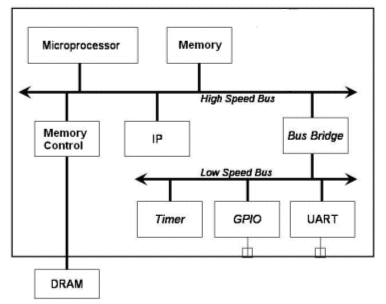
\includegraphics[bb=0 0 386 304,scale=0.5]{./Images/ASIC_BUS.png}
 % 20070430_brazil3.gif: 386x304 pixel, 72dpi, 13.62x10.72 cm, bb=0 0 386 304
 \caption{Βασική μορφή διαύλου.}
\end{figure}
\vspace{0.7cm}


Για την δημιουργία ενός ολοκληρωμένου συστήματος επεξεργασίας εικόνας γίνετε εύκολα αντιληπτό ότι ο δίαυλος επικοινωνίας που θα χρησιμοποιηθεί αποτελεί κυρίαρχο στοιχείο. Επειδή η εργασία που γίνετε στα πλαίσια εκπόνησης διπλωματικής εργασίας και ουσιαστικά συνεχίζει-αναβαθμίζει το έργο που ήδη έχει γίνει στο εργαστήριο Μικροηλεκτρονικής θα πρέπει αρχικά να μελετηθεί το υπάρχων σύστημα που υπάρχει διαθέσιμο. Παρακάτω παρουσιάζεται το διάγραμμα του συστήματος που υπάρχει στο εργαστήριο (κάποιες μονάδες είναι ακόμα στο στάδιο της υλοποίησης από άλλες διπλωματικές).
\newpage
\begin{figure}[h!]
 \centering
 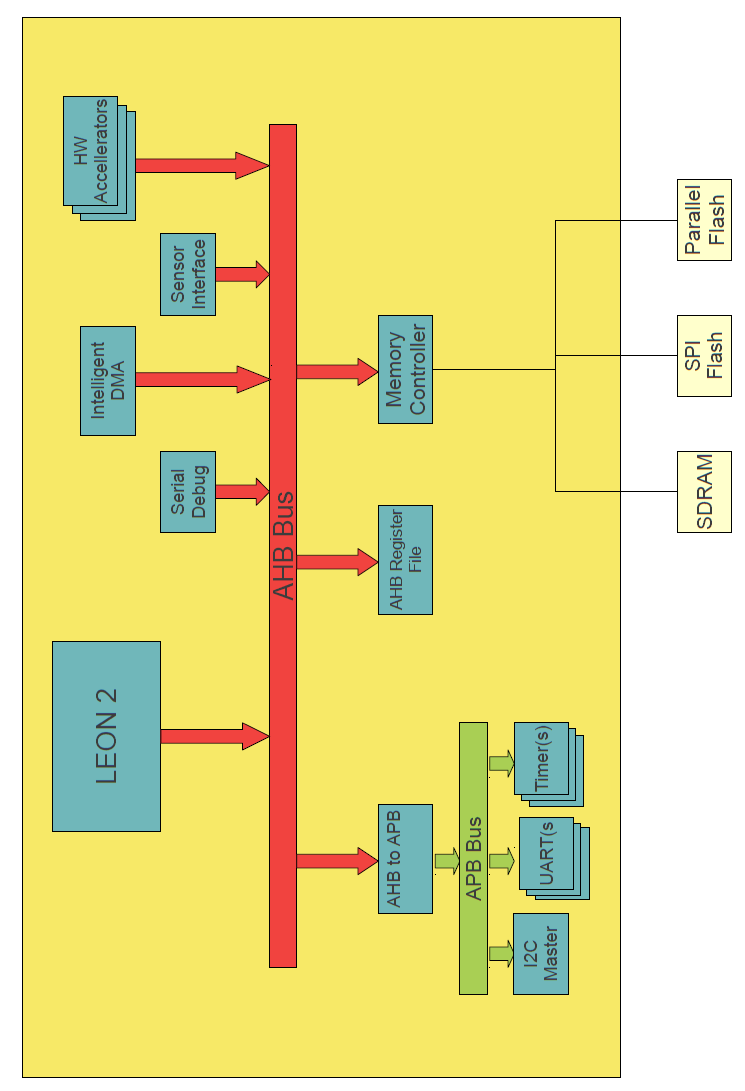
\includegraphics[bb=0 0 745 1091,scale=0.45]{./Images/VLSI_LAB_LEAN2.png}
 % VLSI_LAB_LEAN2.png: 745x1091 pixel, 72dpi, 26.28x38.49 cm, bb=0 0 745 1091
 \caption{Μπλοκ διάγραμμα συστήματος εργαστηρίου.}
\end{figure}
\vspace{0.7cm}
\newpage
Παρατηρώντας το παραπάνω διάγραμμα βλέπουμε ότι το σύστημά μας χρησιμοποιεί το AMBA AHB σαν κεντρικό δίαυλο επικοινωνίας. Σκοπός αυτής της διπλωματικής εργασίας ήταν αναβάθμιση του συστήματος αυτού αντικαθιστώντας τον επεξεργαστή LEON 2 με τον επεξεργαστή OR1200. Αυτό για να μπορεί να είναι υλοποιήσημο πρέπει να σχεδιαστεί μια γέφυρα επικοινωνίας μεταξύ του διαύλου AMBA AHB και του επεξεργαστή OR1200. Ο λόγος ύπαρξης αυτής της γέφυρας οφείλεται στο γεγονός ότι ο επεξεργαστής OR1200 είναι σχεδιασμένος με τέτοιο τρόπο ώστε να είναι άμεσα συμβατός με τον Wishbone δίαυλο και όχι με τον ΑMBA ΑΗΒ. 
\vspace{0.7cm}
\begin{figure}[h!]
 \centering
 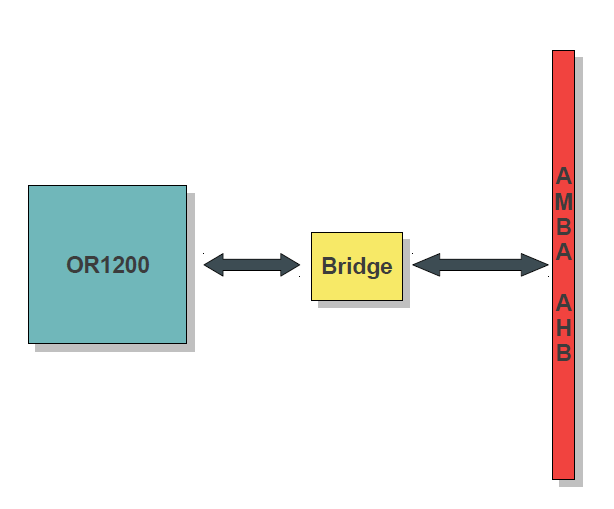
\includegraphics[bb=0 0 614 509,scale=0.5]{./Images/OR1200_br_ahb.png}
 % OR1200_br_ahb.png: 614x509 pixel, 72dpi, 21.66x17.96 cm, bb=0 0 614 509
 \caption{Τοποθεσία Γέφυρας Επικοινωνίας}
\end{figure}
\vspace{0.7cm}

Στις παρακάτω ενότητες θα αναλυθούν τα σήματα που παρέχει τόσο ο δίαυλος AMBA AHB όσο και ο επεξεργαστής OR1200, ο τρόπος με τον οποίο έγινε η σύνδεση τους μέσω της γέφυρας και μια επιτυχημένη μεταφορά δεδομένων μεταξύ του επεξεργαστή και της μνήμης κλείνοντας με αυτόν το τρόπο αυτή την διπλωματική εργασία.

\newpage
\subsection{AMBA AHB Δίαυλος}

Ο δίαυλος επικοινωνίας AMBA AHB είναι ένα προϊόν της εταρείας ARM. Στα σύγχρονα συστήματα ειδικού σκοπού αποτελεί ένα βιομηχανικό στάνταρ η ύπαρξη του. Ο δίαυλος ΑΗΒ είναι ένας δίαυλος που τοποθετείται υψηλότερα (πιο κοντά στο επεξεργαστή) από τον δίαυλο APB και προσφέρει μια πληθώρα από χαρακτηριστικά με στόχο την μεγαλύτερη αποδοτικότητα τους συστήματος. Κάποια από τα χαρακτηριστικά αυτά φαίνονται παρακάτω.
\begin{itemize}
 \item Μεταφορές δεδομένων κατα ριπές.(burst transfers) 
 \item Ξεχωριστές αναμεταδόσεις. (split transactions)
 \item Sigle clock edge operation.
 \item Non-tristate implementation.
 \item Πιο πλατή δίαυλο δεδομένων (65/128 bits).
 \item Single cycle bus master handover.
\end{itemize}

\vspace{0.7cm}
\begin{figure}[h!]
 \centering
 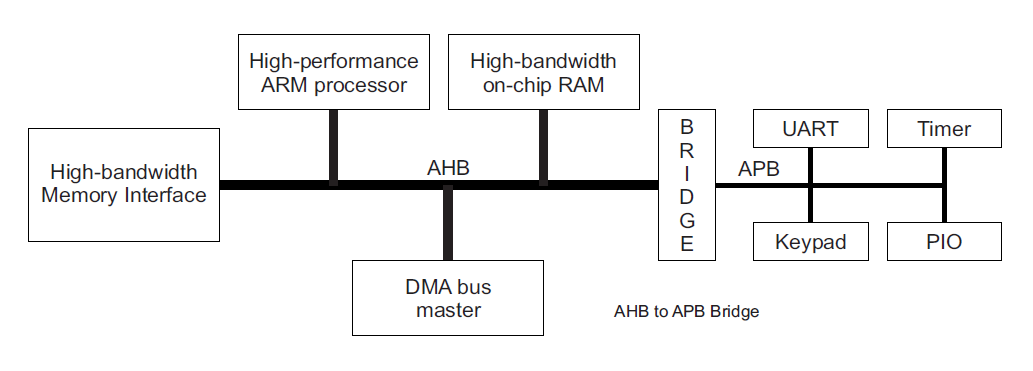
\includegraphics[bb=0 0 1033 371,scale=0.3]{./Images/AHB.png}
 % AHB.png: 1033x371 pixel, 72dpi, 36.44x13.09 cm, bb=0 0 1033 371
 \caption{A typical AMBA AHB-based system}
\end{figure}

Αυτός ο δίαυλος επικοινωνίας είναι εγκατεστημένος στο σύστημα στο οποίο δουλεύουμε. Κατά συνέπεια θα πρέπει να μελετηθεί η λειτουργία του καθώς και τα σήματα που μας παρέχει ώστε να σχεδιάσουμε την γέφυρα επικοινωνίας μεταξύ του επεξεργαστή ΟR1200 και αυτού του διαύλου.
\newline

Σχετικά με την λειτουργία του διαύλου ΑΜΒΑ ΑΗΒ ανατρέξαμε στο εγχειρίδιο που παρέχει η εταιρεία ARM. Όσο αναφορά τα σήματα τα οποία παρέχει και είναι υλοποιημένα στο σύστημα μας φαίνονται παρακάτω.

\newpage

\definecolor{tcA}{rgb}{1,1,0}
\begin{center}
\begin{longtable}{p{1.5 cm} l p{6 cm}}
\caption{AMBA AHB Signals}\\\hline
% use packages: color,colortbl
\rowcolor{tcA}
Name & Source & Description\\\hline
{\bf HCLK}
Bus clock & Clock source & This clock times all bus transfers. All signal
timings are related to the rising edge of {\bf HCLK}.\\\hline
{\bf HRESETn}
Reset & Reset controller & The bus reset signal is active LOW and is used to
reset the system and the bus. This is the only active
LOW signal.\\\hline
{\bf HADDR[31:0]}
Address bus & Master & The 32-bit system address bus.\\\hline
{\bf HTRANS[1:0]}
Transfer type & Master & Indicates the type of the current transfer, which can
be NONSEQUENTIAL, SEQUENTIAL, IDLE or
BUSY.\\\hline
{\bf HWRITE}
Transfer direction & Master & When HIGH this signal indicates a write transfer
and when LOW a read transfer.\\\hline
{\bf HSIZE[2:0]}
Transfer size & Master & Indicates the size of the transfer, which is typically
byte (8-bit), halfword (16-bit) or word (32-bit). The
protocol allows for larger transfer sizes up to a
maximum of 1024 bits.\\\hline
{\bf HBURST[2:0]}
Burst type & Master & Indicates if the transfer forms part of a burst. Four,
eight and sixteen beat bursts are supported and the
burst may be either incrementing or wrapping.\\\hline
{\bf HWDATA[31:0]}
Write data bus & Master & The write data bus is used to transfer data from the
master to the bus slaves during write operations. A
minimum data bus width of 32 bits is
recommended. However, this may easily be
extended to allow for higher bandwidth operation.\\\hline
{\bf HRDATA[31:0]}
Read data bus & Slave & The read data bus is used to transfer data from bus
slaves to the bus master during read operations. A
minimum data bus width of 32 bits is
recommended. However, this may easily be
extended to allow for higher bandwidth operation.\\\hline
{\bf HREADY}
Transfer done & Slave & When HIGH the {\bf HREADY} signal indicates that a
transfer has finished on the bus. This signal may be
driven LOW to extend a transfer.
Note: Slaves on the bus require {\bf HREADY} as both
an input and an output signal.\\\hline
{\bf HRESP[1:0]}
Transfer response & Slave & The transfer response provides additional
information on the status of a transfer.
Four different responses are provided, OKAY,
ERROR, RETRY and SPLIT.\\\hline
{\bf HBUSREQx}
Bus request & Master & A signal from bus master x to the bus arbiter which
indicates that the bus master requires the bus. There is an
{\bf HBUSREQx} signal for each bus master in the system, up to
a maximum of 16 bus masters.\\\hline
{\bf HGRANTx}
Bus grant & Arbiter & This signal indicates that bus master x is currently the
highest priority master. Ownership of the address/control
signals changes at the end of a transfer when {\bf HREADY} is
HIGH, so a master gets access to the bus when both
{\bf HREADY} and {\bf HGRANTx} are HIGH.\\\hline
\end{longtable}
\end{center}

\newpage
\subsection{OR1200 - Wishbone Interface}

Στο κεφάλαιο 2 περιγράφηκαν αναλυτικά οι I/O θύρες που παρέχει ο επεξεργαστής OR1200 εκτός από τις θύρες που χρησιμοποιούνται για την σύνδεση του επεξεργαστή με τον δίαυλο επικοινωνίας. 
\newline

Όπως βλέπουμε στο παρακάτω σχήμα ο επεξεργαστής προσφέρει οι θύρες για την επικοινωνία με τον δίαυλο. Η μια είναι για να μπορούν τα δεδομένα να μεταφέρονται σε άλλες μονάδες και η άλλη είναι για την μεταφορά εντολών. Ο λόγος που έχει δυο θύρες επικοινωνίας οφείλεται στο γεγονός ότι ο επεξεργαστής OR1200 ακολουθώντας την λογική της αρχιτεκτονικής Open Risc 1000 αντιμετωπίζει ξεχωριστά τα δεδομένα και τις εντολές (π.χ ξεχωριστή κρυφή μνήμη για τα δεδομένα από την κρυφή μνήμη των εντολών).

\vspace{0.7cm}
\begin{figure}[h!]
 \centering
 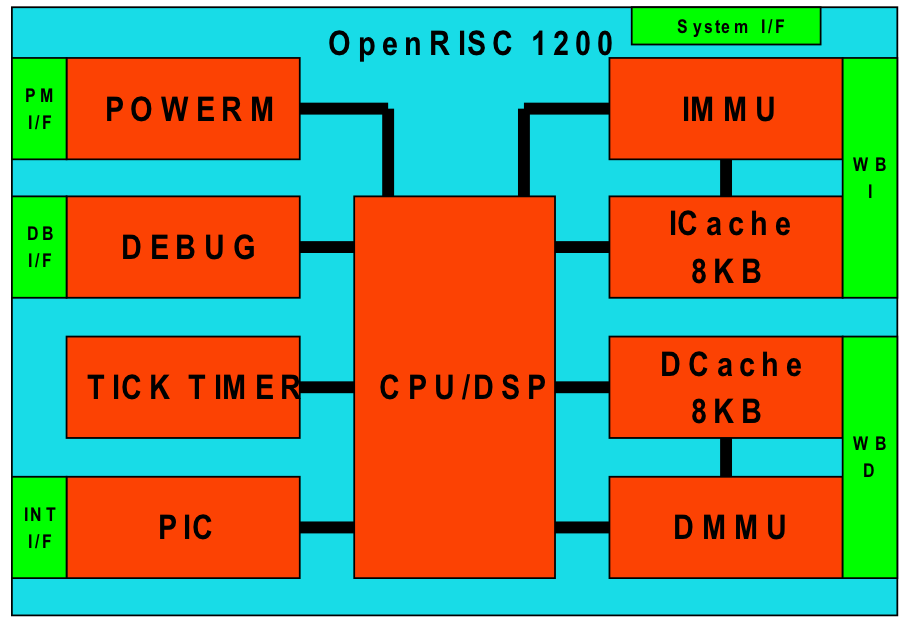
\includegraphics[bb=0 0 905 625,scale=0.3]{/home/federico/Documents/Kile/Diploma/Images/or1200.png}
 % or1200.png: 905x625 pixel, 72dpi, 31.93x22.05 cm, bb=0 0 905 625
 \caption{Core's Architecture}
\end{figure}
\vspace{0.7cm}

O επεξεργαστής OR1200 προσφέρει μια "master" διεπαφή ώστε να μπορεί να συνδέει τον πυρήνα του με το υποσύστημα μνήμης ώστε να προσκομίζει εντολές ή instruction cache lines. Παρακάτω φαίνονται τα σήματα που προσφέρει αυτή η διεπαφή.
\newpage
{%
\vspace{0.7cm}
\renewcommand{\arraystretch}{1.2}
\setlength{\tabcolsep}{0.3em}
\newcommand{\mc}[3]{\multicolumn{#1}{#2}{#3}}
\definecolor{tcA}{rgb}{1,1,0}
\begin{table}[h]
\begin{center}
\begin{tabular}{|l|l|l|p{6 cm}|}
% use packages: color,colortbl
\hline
\rowcolor{tcA}
Port & Width & Direction & Description\\\hline
iwb\_CLK\_I & 1 & Input & Clock input\\\hline
iwb\_RST\_I & 1 & Input & Reset input\\\hline
iwb\_CYC\_O & 1 & Output & Indicates valid bus cycle (core select)\\\hline
iwb\_ADR\_O & 32 & Outputs & Address outputs\\\hline
iwb\_DAT\_I & 32 & Inputs & Data inputs\\\hline
iwb\_DAT\_O & 32 & Outputs & Data outputs\\\hline
iwb\_SEL\_O & 4 & Outputs & Indicates valid bytes on data bus (during valid cycle it must be 0xf)\\\hline
iwb\_ACK\_I & 1 & Input & Acknowledgment input (indicates normal transaction termination)\\\hline
iwb\_ERR\_I & 1 & Input & Error acknowledgment input (indicates an abnormal transaction termination)\\\hline
iwb\_RTY\_I & 1 & Input & In OR1200 treated same way as iwb\_ERR\_I.\\\hline
iwb\_WE\_O & 1 & Output & Write transaction when asserted high\\\hline
iwb\_STB\_O & 1 & Outputs & Indicates valid data transfer cycle\\\hline
\end{tabular}
\end{center}
\caption{Instruction WISHBONE Master Interface’ Signals}
\end{table}
\vspace{0.7cm}
}

O επεξεργαστής OR1200 προσφέρει μια "master" διεπαφή ώστε να μπορεί να συνδέει τον πυρήνα του με το υποσύστημα μνήμης και εξωτερικά περιφερειακά για σκοπούς ανάγνωσης ή εγγραφής δεδομένων και data cache lines. Παρακάτω φαίνονται τα σήματα που προσφέρει αυτή η διεπαφή.
\newpage
{%
\vspace{0.7cm}
\renewcommand{\arraystretch}{1.2}
\setlength{\tabcolsep}{0.3em}
\newcommand{\mc}[3]{\multicolumn{#1}{#2}{#3}}
\definecolor{tcA}{rgb}{1,1,0}
\begin{table}[h]
\begin{center}
\begin{tabular}{|l|l|l|p{6 cm}|}
% use packages: color,colortbl
\hline
\rowcolor{tcA}
Port & Width & Direction & Description\\\hline
dwb\_CLK\_I & 1 & Input & Clock input\\\hline
dwb\_RST\_I & 1 & Input & Reset input\\\hline
dwb\_CYC\_O & 1 & Output & Indicates valid bus cycle (core select)\\\hline
dwb\_ADR\_O & 32 & Outputs & Address outputs\\\hline
dwb\_DAT\_I & 32 & Inputs & Data inputs\\\hline
dwb\_DAT\_O & 32 & Outputs & Data outputs\\\hline
dwb\_SEL\_O & 4 & Outputs & Indicates valid bytes on data bus (during valid cycle it must be 0xf)\\\hline
dwb\_ACK\_I & 1 & Input & Acknowledgment input (indicates normal transaction termination)\\\hline
dwb\_ERR\_I & 1 & Input & Error acknowledgment input (indicates an abnormal transaction termination)\\\hline
dwb\_RTY\_I & 1 & Input & In OR1200 treated same way as dwb\_ERR\_I.\\\hline
dwb\_WE\_O & 1 & Output & Write transaction when asserted high\\\hline
dwb\_STB\_O & 1 & Outputs & Indicates valid data transfer cycle\\\hline
\end{tabular}
\end{center}
\caption{Data WISHBONE Master Interface’ Signals}
\end{table}
\vspace{0.7cm}
}

\newpage
\subsection{Δημιουργία Γέφυρας}
\subsubsection{Θεωρητική ανάλυση}

Μελετώντας τις παραπάνω ενότητες γίνετε αντιληπτό ότι πρέπει να σχεδιαστούν δύο γέφυρες που θα συνδέουν το επεξεργαστή OR1200 με τον δίαυλο επικοινωνίας AMBA AHB. Η μία γέφυρα θα συνδέει την διεπαφή εντολών που παρέχει ο επεξεργαστής και η άλλη θα συνδέει την διεπαφή δεδομένων όπως φαίνεται και στο παρακάτω σχήμα.

\begin{figure}[h!]
 \centering
 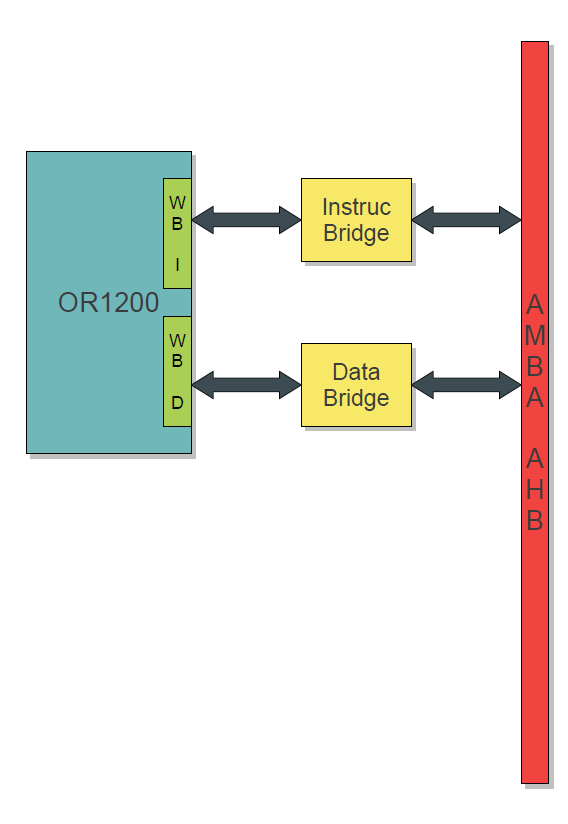
\includegraphics[bb=0 0 568 824,scale=0.5]{./Images/or1200-br-ahb.png}
 % or1200-br-ahb.png: 568x824 pixel, 72dpi, 20.04x29.07 cm, bb=0 0 568 824
 \caption{Τοποθεσία γεφυρών στο σύστημα μας}
\end{figure}


\vspace{0.7cm}

Οι δυο αυτές γέφυρες θα είναι με το ίδιο τρόπο υλοποιημένες άπλα χρείαζονται δύο τέτοιες υπομονάδες για να πετύχουμε την σύνδεση του OR1200 με τον δίαυλο επικοινωνίας.
\newline

Για την υλοποίηση αυτών των γεφυρών επικοινωνίας χρησιμοποιήθηκε σαν βάση μια ήδη υπάρχουσα υλοποίηση  από την εταιρεία TooMuch Semiconductor \newline Solutions που παρέχεται ελεύθερα από το Open Cores.
Η συγκεκριμένη γέφυρα προσφέρει την απαραίτητη λογική ώστε να μπορεί να γίνει η σύνδεση του επεξεργαστή με τον δίαυλο με τέτοιο τρόπο ώστε να μπορούν να γίνονται απλές μεταφορές δεδομένων μεταξύ του επεξεργαστή και των άλλων υπομονάδων του συστήματος μας.
Κάποιοι περιορισμοί που υπάρχουν σε αυτήν την υλοποίηση αλλά δεν αποτελούν πρόβλημα για την δική μας περίπτωση φαίνονται παρακάτω.
\begin{itemize}
 \item Ο σχεδιασμός αυτός δεν υποστηρίζει την διαδοχική μεταφορά δεδομένων. Αντίθετα μπορεί να μεταφέρει μεγάλα μπλοκ δεδομένων θεωρώντας όμως ότι δεν είναι διαδοχικές μεταφορές δεδομένων.
 \item Η λέξη (word) έχει μέγεθος 32 bits.
 \item Δεν υποστηρίζονται οι καταστάσεις λάθους, επανάληψης και διαχωρισμός (error, retry and split).
\end{itemize}

Το μπλόκ διάγραμμα που περιγράφει την γέφυρα επικοινωνίας καθώς και τα σήματα που χρησιμοποιούνται φαίνονται παρακάτω.

\begin{figure}[h!]
 \centering
 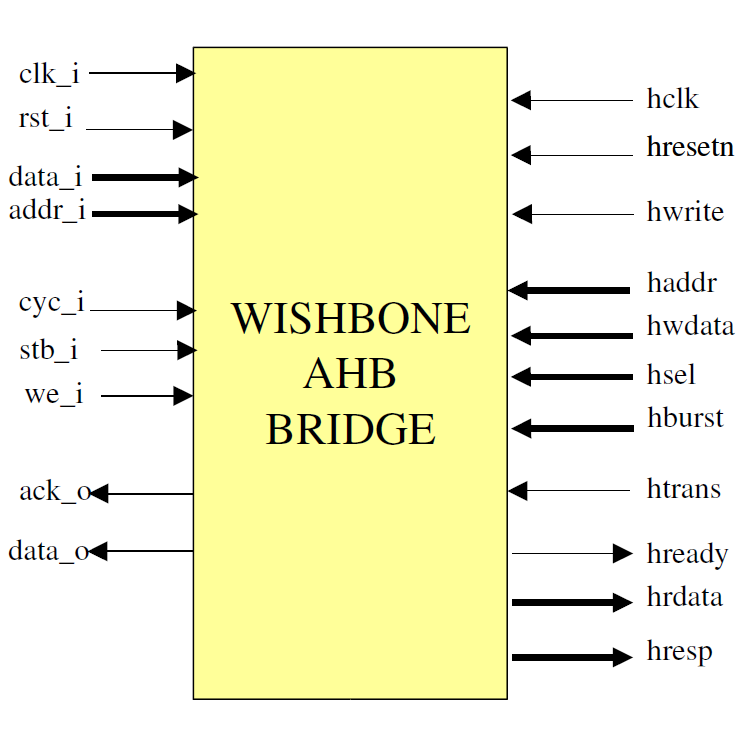
\includegraphics[bb=0 0 756 730,scale=0.4]{./Images/ahb_wb_ORIG.png}
 % ahb_wb_ORIG.png: 756x730 pixel, 72dpi, 26.67x25.75 cm, bb=0 0 756 730
 \caption{Μπλοκ διαγραμμα γέφυρας επικοινωνίας.}
\end{figure}


{%
\vspace{0.7cm}
\renewcommand{\arraystretch}{1.2}
\setlength{\tabcolsep}{0.3em}
\newcommand{\mc}[3]{\multicolumn{#1}{#2}{#3}}
\definecolor{tcA}{rgb}{1,1,0}
\begin{table}[h]
\begin{center}
\begin{tabular}{|l|l|l|l|p{6 cm}|}
% use packages: color,colortbl
\hline
\rowcolor{tcA}
Port Name & Direction & Size  & Sourse & Description\\\hline
haddr & out  & 32 & AHB Master & Address Bus\\\hline
htrans & out & 2 & AHB Master & Transfer Type\\\hline
hwrite & out & 1 &AHB Master & Read/Write enable\\\hline
hsize & out & 3 & AHB Master & not used\\\hline
hburst& out & 3 & AHB Master & Burst Type\\\hline
hwdata & out & 32 & AHB Master & Write data bus\\\hline
hrdata & out & 32 & AHB Master & Read data bus\\\hline
hready & in  & 32 & AHB Slave & To indicate bridge is ready\\\hline
hresp & in & 2 & AHB Slave & Response\\\hline
data\_o & out & 32 & WISHBONE Slave & Read data bus\\\hline
data\_i & in & 32 & WISHBONE Master & Write data bus\\\hline
addr\_i & in & 32 & WISHBONE Master & Address Bus\\\hline
clk\_i & in & 1 & WISHBONE Master & Clock\\\hline
rst\_i& in & 1 & WISHBONE Master & Active Hign Sync. Reset\\\hline
cyc\_i & in  & 1 & WISHBONE Master & To indicate valid bus cycle\\\hline
stb\_i & in & 1 & WISHBONE Master & To indicate valid data transfer cycle\\\hline
sel\_i & in & 4 &WISHBONE Decoder & Selection\\\hline
we\_i & in & 1 & WISHBONE Master & Read/Write enable\\\hline
ack\_o & out & 1 & WISHBONE Slave & To indicate current transfer status\\\hline
hclk & in & 1 & AHB Master & Unconnected\\\hline
hresetn & in & 1 & AHB Master & Unconnected\\\hline
\end{tabular}
\end{center}
\caption{Σήματα γέφυρας επικοινωνίας.}
\end{table}
\vspace{0.7cm}
}%
\newpage
Παρατηρώντας τα παραπάνω σήματα που παρέχει αυτή η γέφυρα βλέπουμε να λείπουν τα σήματα \emph{hbusreq} και \emph{hgrantx} που χρησιμοποιεί η δικιά μας υλοποίηση του δίαυλου AMBA AHB. Αυτά τα σήματα χρησιμοποιούνται όταν πάνω στον δίαυλο επικοινωνίας τοποθετούνται παραπάνω από μία μονάδες που θα πρέπει να ανταγωνίζεται η μία την άλλη για να αποκτήσει πρόσβασή πάνω στο δίαυλο. Ουσιαστικά το \emph{hbusreq} είναι ένα σήμα που δέχεται ο δίαυλος AHB από κάποια μονάδα master όταν αυτή η μονάδα θέλει να αποκτήσει πρόσβαση πάνω στον δίαυλο. Το αντίστοιχο σήμα που στέλνει ο επεξεργαστής OR1200 όταν επιθυμεί να αποκτήσει πρόσβασή πάνω στον δίαυλο είναι το \emph{dwb\_CYC\_O} για μεταφορά δεδομένων και το \emph{iwb\_CYC\_O} για μεταφορά εντολών. Επειδή όπως προαναφέρθηκε και οι δυο γέφυρες επικοινωνίας θα έχουν την ίδια υλοποίηση τόσο για αυτήν που θα συνδεθεί με την διεπαφή δεδομένων όσο και αυτή με την διεπαφή εντολών τα σήματα θα αναγράφονται με * μπροστά από την ονομασία τους αντί για \emph(i) ή \emph(d) αντίστοιχα. Δηλαδή στην προκειμένη περίπτωση \emph{*wb\_CYC\_O}. Άρα για να υλοποιεί η γέφυρα επικοινωνίας τους σκοπούς αυτών των δύο σημάτων πρέπει μέσα στην γέφυρα να ενώνονται αυτά και όταν ο επεξεργαστής θέλει αν αποκτήσει πρόσβαση στον δίαυλο (ενεργοποιώντας το σήμα \emph{*wb\_CYC\_O}) τότε αυτό το σήμα θα οδηγείται στην γέφυρα και εκείνη με την σειρά της θα  θα ενεργοποιεί το σήμα \emph{hbusreq} που θα οδηγείται πάνω στον δίαυλο και θα μεταφέρει ουσιαστικά το αίτημα του επεξεργαστή.


Το άλλο σήμα που και αυτό δεν υλοποιείται  είναι το \emph{hgrantx}. Ουσιαστικά αύτο το σήμα είναι το αποτέλεσμα του σήματος \emph{hbusreq}. Δηλαδή όπως αναφέρθηκε και παραπάνω όταν το \emph{hbusreq} ενεργοποιηθεί τότε ο δίαυλος με την βοήθεια του διαιτητή (arbiter) πρέπει να ενεργοποιήσει το σήμα \emph{hgrantx} στην αντίστοιχη μονάδα που το αιτήθηκε ώστε να να της επιτρέψει να αναλάβει τον έλεγχο του διαύλου. Από την στιγμή που αναλάβει τον έλεγχο τότε όταν και το \emph{hready} ενεργοποιηθεί θα πραγματοποιήσει την μεταφορά.

Η παραπάνω λογική ενσωματώνεται στην γέφυρα μας προσθέτοντας το σήμα \emph{hgrant} σαν είσοδο στην γέφυρα μας και συνδέοντας το με το \emph{hgrantx} του διαύλου. Εσωτερικά στην γέφυρα περνάμε τα σήματα \emph{hgrant} και \emph{hready} από μία λογική πύλη AND της οποίας την έξοδο την ανατροφοδοτούμε στο σήμα εξόδου της γέφυρας \emph{ack\_o}. Αυτό το σήμα (\emph{ack\_o}) επειδή συνδέεται με το σήμα \emph{*wb\_ACK\_I} του επεξεργαστή έχει σαν αποτέλεσμα όταν ενεργοποιείται να ξεκινάει η μεταφορά δεδομένων, που ουσιαστικά είναι η επιθυμητή κατάσταση. Ταυτόχρονα για ασφάλεια βάζουμε όλες τις συναρτήσεις που υλοποιούνται στην γέφυρα μέσα σε ένα \underline{if (hgrant and hready) do then fuctions} ώστε να ξεκινάει η λειτουργία της γέφυρας όταν τόσο το \emph{hgrant} όσο και το \emph{hready} είναι ενεργοποιημένα. Με αυτό τον τρόπο αποφεύγουμε την άσκοπη λειτουργία της γέφυρας.

Τέλος τα σήματα \emph{*wb\_ERR\_I} και \emph{*wb\_RTY\_I} του επεξεργαστή τα οδηγούμε στο 0 μίας και η υλοποίηση τους δεν ήταν μέρος της διπλωματικής. Ο λόγος που τα οδηγούμε στο 0 είναι ότι με αυτό τον τρόπο εξασφαλίζουμε ότι ποτέ δεν θα φτάσει αίτημα στον επεξεργαστή για επανάληψη μεταφοράς δεδομένων ή σε περίπτωση λάθους.

\subsubsection{Υλοποίηση σε Verilog}

Ουσιαστικά σε αύτη την ενότητα θα παρουσιάσουμε υλοποίηση σε κώδικά Verilog των λειτουργιών που περιγράφηκαν παραπάνω. Παρακάτω βρίσκετε ο κώδικας που δημιουργήθηκε σχολιασμένος.
\vspace{0.7cm}
\lstinputlisting{/home/federico/Documents/Kile/Diploma/ahbmas_wbslv_top.v} 


\newpage
\section{Υλοποίηση Συστήματος}

\subsection{Συνδεσμολογία συστήματος}
Σκοπός αυτής της διπλωματικής εργασίας είναι να δημιουργήσουμε ένα ολοκληρωμένο σύστημά για την επεξεργασία εικόνας. Αυτό βέβαια προϋποθέτει την ύπαρξη και την σχεδίαση άλλων υπομονάδων από ένα σύνολο ανθρώπων. Για αυτό τον λόγο επειδή κάποια κομμάτια δεν είναι έτοιμα ακόμα σχεδιάστηκε μια πιο απλή μορφή συστήματος που αποδεικνύει την σωστή λειτουργία όσων αναφέρθηκαν στις προηγούμενες ενότητες. Το σύστημα που δημιουργήθηκε φαίνεται παρακάτω.

\vspace{0.7cm}
\begin{figure}[h!]
 \centering
 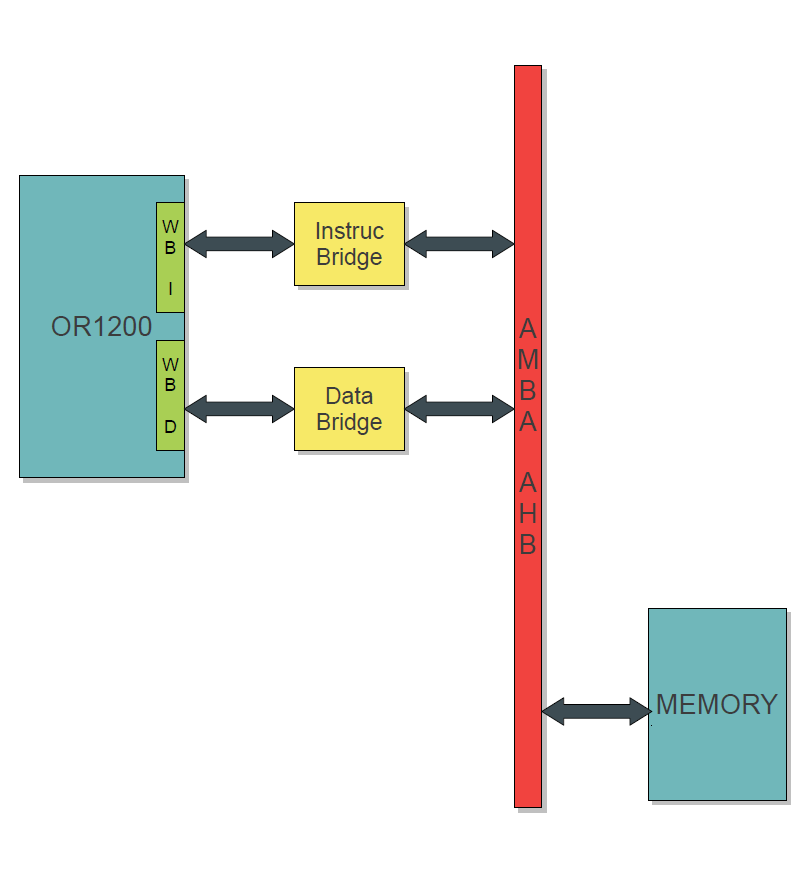
\includegraphics[bb=0 0 806 871,scale=0.42]{./Images/or1200_D_I_wb_ahb_mem.png}
 % or1200_D_I_wb_ahb_mem.png: 806x871 pixel, 72dpi, 28.43x30.73 cm, bb=0 0 806 871
 \caption{Σύστημα.}
\end{figure}
\newpage

Όπως φαίνεται στο παραπάνω σχήμα το σύστημα μας αποτελείται:
\begin{itemize}
 \item To επεξεργαστή OR1200.
 \item Τις δύο γέφυρες επικοινωνίας.
 \item Τον δίαυλο επικοινωνίας AMBA AHB.
 \item Μια τυπική μνήμη.
\end{itemize}



Ουσιαστικά με αυτό το σύστημα μπορούμε να ελένξουμε τόσο την σωστή λειτουργία του επεξεργαστή όσο και την λειτουργία των γεφυρών επικοινωνίας.

Στόχος μας είναι να πραγματοποιήσουμε απλές μεταφορές δεδομένων από και προς την μνήμη. Με αυτό τον τρόπο εξασφαλίζουμε τόσο την αρμονική λειτουργία του επεξεργαστή με τις γέφυρες όσο και την ορθή επικοινωνία των γεφυρών με δίαυλο AMBA AHB. Να σημειωθεί σε αυτό το σημείο ότι δημιουργία του διαύλου AMBA ΑΗΒ και της μνήμης έγινε από Κώστα Αδαό που είναι υπεύθυνος του εργαστηρίου Μικροηλεκτρονικής.
\newline

Στα παρακάτω σχέδια παρουσιάζεται η συνδεσμολογία που δημιουργήθηκε μεταξύ του επεξεργαστή OR1200, των γεφυρών επικοινωνίας και του διαύλου ΑΜΒΑ ΑΗΒ.
\newpage
\begin{figure}[h!]
 \centering
 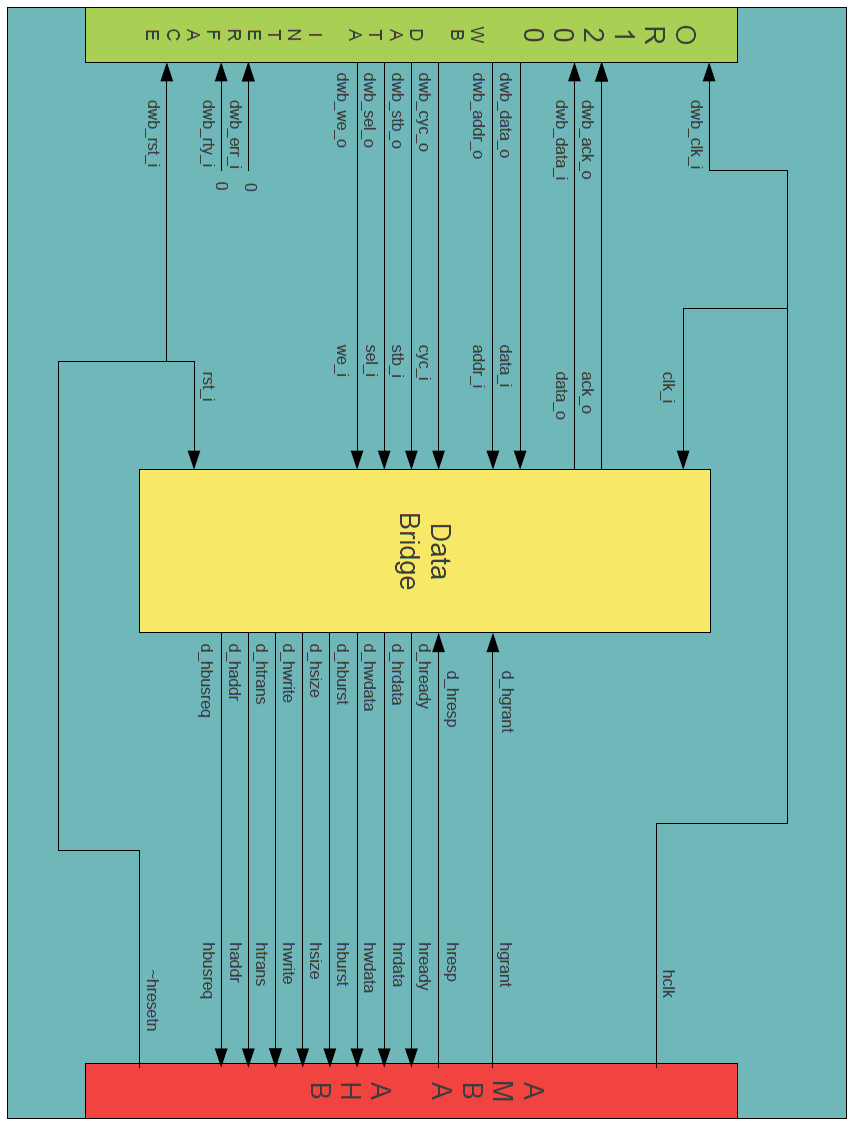
\includegraphics[bb=0 0 851 1125,scale=0.41]{./Images/signals_D.png}
 % signals_D.png: 851x1125 pixel, 72dpi, 30.02x39.69 cm, bb=0 0 851 1125
 \caption{Συνδεσμολογία Γεφυρας δεδομένων}
\end{figure}
\newpage

\begin{figure}[h!]
 \centering
 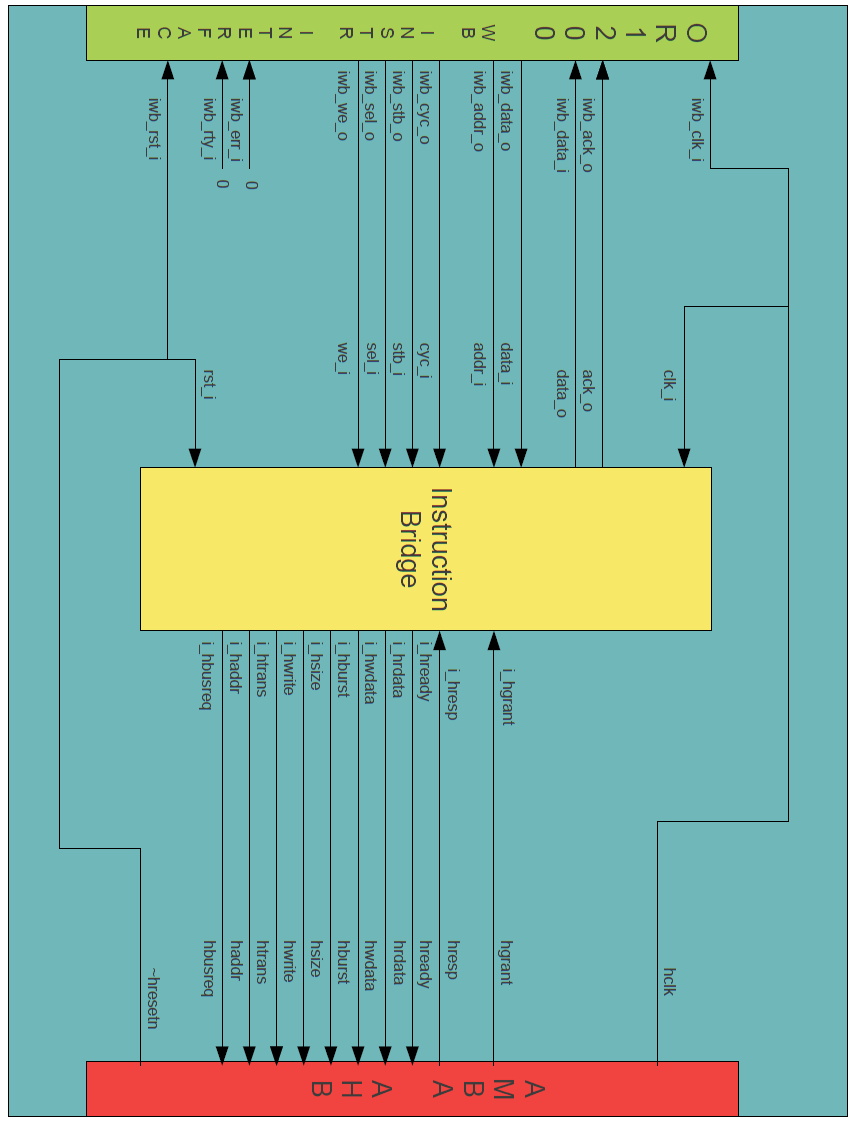
\includegraphics[bb=0 0 851 1125,scale=0.41]{./Images/signal_I.png}
 % signals_D.png: 851x1125 pixel, 72dpi, 30.02x39.69 cm, bb=0 0 851 1125
 \caption{Συνδεσμολογία Γεφυρας Εντολών}
\end{figure}

\newpage
\subsection{Προσομοίωση Συστήματος}

Για να γίνει η προσομοίωση του παραπάνω συστήματος αφού δημιουργήθηκε από το κ.Αδαό ο δίαυλος επικοινωνίας και η μνήμη στο αρχειο \emph{ahb\_test\_final} ακολουθήθηκαν βήματα που περιγράφονται παρακάτω.
\newline

\paragraph{1. Προσθήκη κατάλληλων αρχείων Verilog \newline\newline}

Αρχικά προστέθηκε μέσα στον φάκελο \emph{ahb\_test\_final} ένας καινούργιος φάκελος με την ονομασία \emph{or1200\_top\_ahb} μέσα στον οποίο είναι τοποθετημένο το top αρχείο που περιγράφει την λειτουργία της γέφυρας καθώς και το initialization  του επεξεργαστή OR1200 που ουσιαστικά συνδέει όλα τα σήματα που του OR1200 με τέτοιο τρόπο ώστε να καλύπτει τις ανάγκες του συστήματος. Το αρχείο αυτό έχει την ονομασία \emph{or1200\_top\_ahb.v} και παρακάτω βρίσκεται ο σχολιασμένος κώδικας που σχεδιάστηκε.


\vspace{0.7cm}
\lstinputlisting{/home/federico/Documents/Kile/Diploma/or1200_top_ahb.v} 
\newpage


\paragraph{2. Τροποποίηση testbench\newline\newline}

Ακολουθώντας την μεθοδολογία που περιγράφηκε στο τρίτο κεφαλαίο κάναμε μερικές εξομοιώσεις και εξάγαμε το παρακάτω συμπέρασματα.
\begin{itemize}
 \item Όταν ξεκίνα την λειτουργία του ο επεξεργαστής παίρνει δεδομένα από την μνήμη χρησιμοποιώντας την διεπαφη εντολών.
 \item Οι πρώτες 3 διευθύνσεις που προσπελαύνει είναι οι 00000100, 00000104 και 00000108. Απο αυτές τις διευθύνσεις παίρνει τα δεδομένα που έχουν μεσά.
\end{itemize}

Εκμεταλλευόμενοι τα παραπάνω συμπεράσματα και λαμβάνοντας υπόψιν τον σκοπό αυτή της διπλωματικής εργασίας δημιουργήσαμε ένα testbech που αρχικά θα βάζει στις παραπάνω διευθύνσεις της μνήμης κάποια δεδομένα που εμείς επιλέξαμε και μετά θα ενεργοποιεί τον επεξεργαστή και θα περιμένουμε λογικά να τραβήξει αυτά τα δεδομένα από την μνήμη μέσω της γέφυρας εντολών ο επεξεργαστής OR1200.
\newline
Αυτό έγινε τροποποιώντας το αρχείο \emph{ahb\_master.v} που βρίσκεται μέσα στο φάκελο \emph{ahb\_test\_final/ahb\_models/} όπως φαίνεται παρακάτω.
\newline
\begin{lstlisting}

task ahb_master_commands;
    begin

        #1_000;
        
        repeat(200) @(posedge hclk);
        
        set_size(BUS_32); $display;
        raddr = 32'h0000_0100; ahb_write(raddr, 32'h1234_5678, 1);
        raddr = 32'h0000_0104; ahb_write(raddr, 32'h0000_0001, 1);
        raddr = 32'h0000_0108; ahb_write(raddr, 32'h9999_9999, 1);

    
    end

endtask

\end{lstlisting}


\paragraph{3. Τροποποίηση Makefile\newline\newline}
Μετά την τοποθέτηση των κατάλληλων αρχείων Verilog προστέθηκαν οι παρακάτω γραμμές κώδικα μέσα στο αρχείο \emph{Makefile} που βρίσκεται μέσα στο φάκελο \emph{ahb\_test\_final} μέσα στο section \underline{sim:}.
\vspace{0.7cm}
\begin{lstlisting}
	or1200_top_ahb/or1200_top_ahb.v \
	or1200_top_ahb/ahbmas_wbslv_top.v \
	-y rtl/verilog/or1200    \
	+incdir+../orpsocv2/rtl/verilog/include \
	+libext+.v \
	-y ../orpsocv2/rtl/verilog/or1200    \
	+incdir+/mnt/datafs/users/kalargaris/orpsocv2/sim/run/../../
bench/verilog/include \
\end{lstlisting}
\vspace{0.7cm}
Το παραπάνω Makefile ελέγχει την ροή προσομοίωσης όποτε αυτό που κάναμε ήταν να συμπεριλάβουμε τα αρχεία που περιγράφουν τον επεξεργαστή καθώς και τα τεστ του επεξεργαστή όπως φαίνεται παραπάνω.

\paragraph{4. Στάδιο Προσομοίωσης \newline\newline}

Για να γίνει η προσομοίωση εκτελέστηκαν οι παρακάτω εντολές με την σειρά που αναγράφονται μέσα στον φάκελο \emph{or1200\_top\_ahb} με την βοήθεια του terminal.
\vspace{0.7cm}
\begin{lstlisting}
make clean
#clean directories from results from previus simulations
\end{lstlisting}
\vspace{0.7cm}
\begin{lstlisting}
make sim
#to simulate ouy system
\end{lstlisting}
\vspace{0.7cm}



\paragraph{5. Προβολή Κυματομορφών - Σχολιασμός \newline\newline}

Με την παρακάτω εντολή μπορούμε να δούμε τις κυματομορφές της προσομοίωσης που κάναμε παραπάνω και να διαπιστώσουμε αν το σύστημα μας λειτουργεί αρμονικά.

\vspace{0.7cm}
\begin{lstlisting}
make waves
# to open waveforms with simvision
\end{lstlisting}
\vspace{0.7cm}

Εκτελώντας την παραπάνω εντολή παίρνουμε τις παρακάτω κυματομορφές. Να σημειωθεί ότι επιλέχθηκαν μόνο εκείνα τα σήματα που χρειάζονταν να αναπαρασταθούν ώστε να δείξουμε την αρμονική λειτουργία του συστήματος. Δηλαδή οτί ξεκινά ο επεξεργαστής την λειτουργία του και αλληλεπιδρά σωστά με την μνήμη όπως ορίσαμε στο τρίτο βήμα παραπάνω.

\begin{figure}[h!]
 \centering
 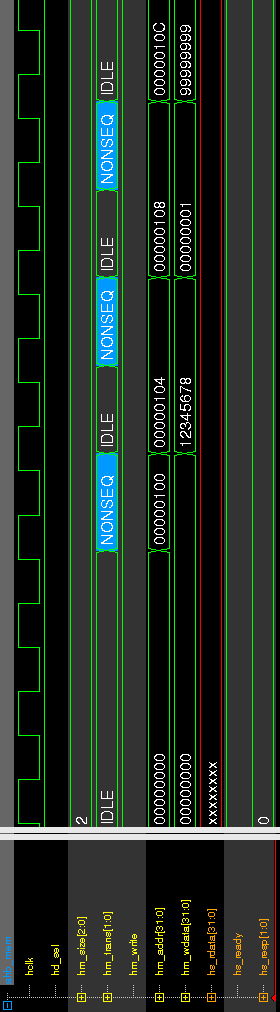
\includegraphics[bb=0 0 280 1012,scale=0.45]{./Images/waves_mem.png}
 % waves_mem.png: 280x1012 pixel, 72dpi, 9.88x35.70 cm, bb=0 0 280 1012
 \caption{Κυματομορφή λειτουργίας μνήμης.}
\end{figure}

\newpage
Στην παραπάνω κυματομορφή εμφανίζεται η λειτουργία της μνήμης. Βρισκόμαστε στο αρχικό στάδιο που γράφουμε στην μνήμη στις διευθύνσεις 00000100, 00000104 και 00000108 τα δεδομένα 12345678, 00000001 και 99999999 αντίστοιχα.

Παρατηρούμε ότι γίνετε εγγραφή αφού χρησιμοποιείται το σήμα \emph{hwdata} που υποδηλώνει την εγγραφή και το σήμα \emph{hrdata} που υποδηλώνει την ανάγνωση.
\newline

Η παρακάτω κυματομορφή δείχνει την λειτουργία του επεξεργαστή όταν θέλει να προσπελάσει τα δεδομένα στην μνήμη.
\newpage
\begin{figure}[h!]
 \centering
 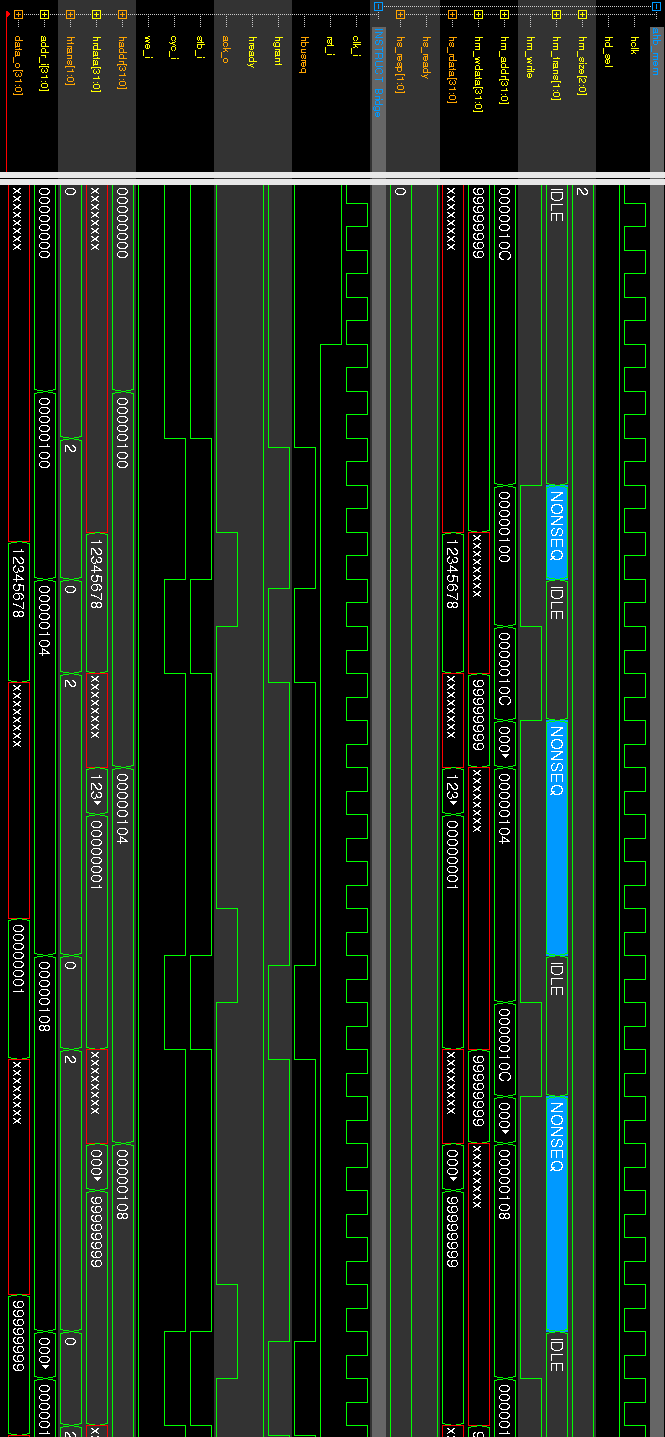
\includegraphics[bb=0 0 665 1437,scale=0.38]{./Images/waves_I_BR_FINAL.png}
 % waves_I_BR_FINAL.png: 665x1437 pixel, 72dpi, 23.46x50.69 cm, bb=0 0 665 1437
 \caption{Κυματομορφή λειτουργίας προσπέλασης.}
\end{figure}
\newpage

Επειδή είναι δύσκολο να σχολιαστεί αυτή η κυματομορφή παρακάτω παρουσιάζεται η επεξεργασμένη κυματομορφή που θα μας βοηθήσει να σχολιάσουμε την λειτουργία.

\begin{figure}[h!]
 \centering
 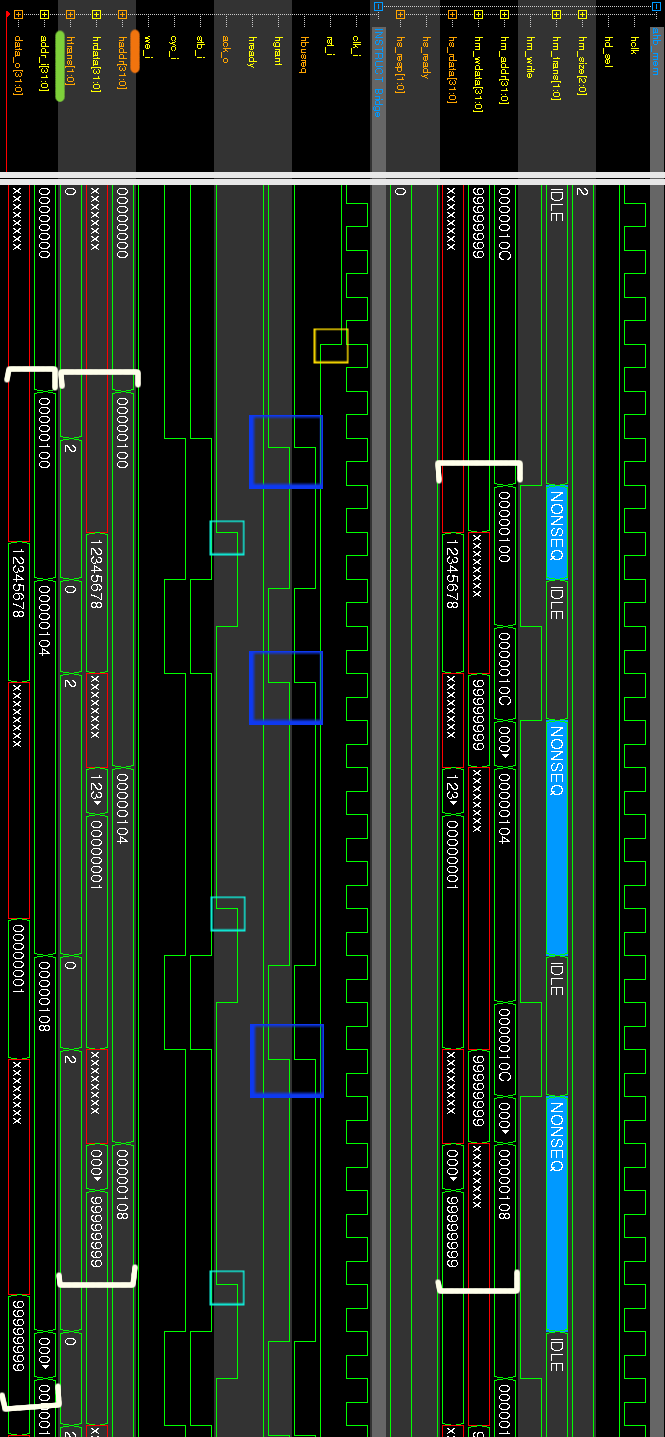
\includegraphics[bb=0 0 665 1437,scale=0.3]{./Images/waves_I_BR_FINAL1.png}
 % waves_I_BR_FINAL1.png: 665x1437 pixel, 72dpi, 23.46x50.69 cm, bb=0 0 665 1437
 \caption{Επεξεργασμένη κυματομορφή.}
\end{figure}
\newpage
\vspace{0.7cm}
\vspace{0.7cm}
Παρατηρώντας την παραπάνω κυματομορφή διακρίνουμε τα εξής χαρακτηριστικά που δηλώνουν την σωστή λειτουργία τους συστήματος μας.
\begin{enumerate}
 \item \underline{Κίτρινο τετράγωνο:} Εδώ παρατηρούμε το σήμα \emph{rst\_i} που όταν απενεργοποιείται ουσιαστικά ενεργοποιεί τον επεξεργαστή και την γέφυρα.
 \item \underline{Μπλε τετράγωνο:} Εδώ παρατηρούμε τα σήματα \emph{hbusreq},\emph{hready} και \emph{hgrant}. Ουσιαστικά αφου ξεκίνησε ο επεξεργαστής απαιτεί πρόσβαση στο δίαυλο
ενεργοποιώντας το σήμα \emph{cyc\_i}. Αυτό το σήμα μεταφέρεται διαμέσου της γέφυρας εντολών στον δίαυλο με την ενεργοποίηση του σήματος \emph{hbusreq}. Παρατηρούμε ότι ο δίαυλος του επιστρέφει αμέσως την έγκριση πρόσβασης στο δίαυλο με την ενεργοποίηση του σήματος \emph{hgrant} και συνδυασμός με το σήμα \emph{hready} παρατηρούμε την ενεργοποίηση του σήματος \emph{ack\_o}.
 \item \underline{Γαλάζιο τετράγωνο:} Εδώ παρατηρούμε το σήμα \emph{ack\_o} που ενεργοποιείται όπως αναφέραμε παραπάνω και ουσιαστικά λέει στον επεξεργαστή να ξεκινήσει την μεταφορά δεδομένων.
 \item \underline{Πορτοκαλί υπογράμμιση:} Εδώ παρατηρούμε το σήμα \emph{we\_i} που είναι απενεργοποιημένο. Αυτό δείχνει ότι θα εκτελεστούν αναγνώσεις από την μνήμη και όχι εγγραφές σε αυτήν.Πράγμα το οποίο περιμέναμε ουσιαστικά.
 \item \underline{Άσπρες αγκύλες:} Ουσιαστικά τα σήματα που περιέχουν αυτές οι αγκύλες παρουσιάζουν την λειτουργίας της μεταφοράς δεδομένων. Αρχικά στο σήμα \emph{addr\_i[31:0]} o επεξεργαστής τοποθετεί την διεύθυνση της μνήμης από την οποία θέλει να πάρει τα δεδομένα. Μέτα αυτό πηγαίνει στην γέφυρα και η οποία βγάζει σαν έξοδο το σήμα \emph{haddr[31:0]} που περιέχει την διεύθυνση μνήμης και την τοποθετεί πάνω στον δίαυλο επικοινωνίας. Ύστερα ο δίαυλος επικοινωνίας μεταφέρει αυτό το σήμα σαν είσοδο στην μνήμη στο σήμα \emph{hm\_addr[31:0]}. Μετά η μνήμη παίρνει τα δεδομένα που βρίσκονται σε αυτή την διεύθυνση και τα μεταφέρει στο σήμα \emph{hs\_rdata[31:0]} που χρησιμοποιείται μόνο για σκοπούς ανάγνωσης. Ύστερα αυτό το σήμα που περιέχει τα δεδομένα που θέλουμε μεταφέρεται διαμέσου του διαύλου στον γέφυρα εντολών η οποία με την σειρά της το μεταφέρει στον επεξεργαστή διάμεσου του σήματος \emph{data\_o[31:0]} οπότε και φτάνουν τα δεδομένα που είχε ζητήσει ο επεξεργαστής αρχικά σε αυτόν.
 \item \underline{Πράσινη υπογράμμιση:} Εδώ παρατηρούμε το σήμα \emph{htrans[1:0]} που περιγράφει το είδος της μεταφοράς. Όταν έχει την τιμή 2 τότε πραγματοποιείται μια απλή μεταφορά δεδομένου (Nonseq transfer) και όταν είναι 0 δείχνει ότι δεν πραγματοποιείται εκείνη την στιγμή κάποια μεταφορά.
\end{enumerate}
\vspace{1.7cm}
Συνοψίζοντας τα παραπάνω συμπεράσματα από τις κυματομορφές μπορούμε να διαπιστώσουμε ότι ο επεξεργαστής OR1200 λειτουργεί αρμονικά με την μνήμη που ήταν και ο αρχικός μας στόχος. Υπάρχουν πολλά περιθώρια βελτίωσης των παραδειγμάτων που αναφέρθηκαν σε αυτήν την διπλωματική άλλα με την χρήση πιο σύνθετων παραδειγμάτων δεν θα ήταν εύκολο να αναλυθεί η λειτουργία του συστήματος μας. Μέτα την παραπάνω υλοποίηση έχει σχεδιαστεί η ραχοκοκκαλιά του συστήματος πάνω στο οποίο θα μπορέσουν μελλοντικά οι φοιτητές να τοποθετήσουν τις δικές τους μονάδες.

%################################################
%#              BIBLIOGRAPHY                    #
%################################################
\newpage
\vspace{0.7cm}
\newpage
\begin{thebibliography}{9}

\bibitem{lamport92}
  ARM Holdings plc, \emph{ “AMBA™ Specification (Rev 2.0)”,}
Released:May 13, 1999.  \url{www.arm.com}.

\bibitem{lamport89}
Damjan Lampret, \emph{“OpenRISC 1200 IP Core Specification”,} Rev. 0.11,
Released:January, 2011. 

\bibitem{lamport88}
  Deepak Kumar Tala, \emph{ “Verilog Tutorial”,}
Released:October 25, 2003. 

\bibitem{lamport85}
 Helmut Kopka, Patrick W. Daly, \emph{A Guide to \LaTeX  and Electronic Publishing,}
  Addison-Wesley Publishing Company,
  Fourth edition,
  Released:2004.

\bibitem{lamport90}
Julius Baxter, OpenCores Organization, \emph{ “ORPSoC User Guide”,}
Released:2010.  \url{www.opencores.org}.

\bibitem{lamport91}
Mattsson, Christensson, \emph{ “Evaluation of synthesizable CPU cores”,}
Master’s Thesis, Chalmers University of Technology, 2004.

\bibitem{lamport87}
  OpenCores Organization, \emph{“OpenRISC 1000 Architecture Manual”,}
Released:April 5, 2006.  \url{www.opencores.org}.

\bibitem{lamport87}
  OpenCores Organization, \emph{“OpenCores HDL modeling guidelines”,}
Released:2009.  \url{www.opencores.org}.

\bibitem{lamport93}
  Richard Herveille, OpenCores Organization, \emph{ “WISHBONE System-on-Chip (SoC) Interconnection
Architecture for Portable IP Cores”, Revision: B.3,}
Released:September 7, 2002.  \url{www.opencores.org}.

\bibitem{lamport88}
  TooMuch Semiconductor Solutions, \emph{“WISHBONE-AHB BRIDGE”,} Rev. 1.0,
Released:2007. 

\bibitem{lamport86}
  Vinayak Pai, Swapnil S. Lotlikar, \emph{“Modeling Lifetime Reliability of Processor Cores”,}
Department of ECE,Texas A\&M University,College Station, Texas.

\end{thebibliography}


\end{document}